\documentclass{book}

\usepackage[utf8]{inputenc}
\usepackage{amsmath}
\usepackage{amsthm}
\usepackage{amssymb}
\usepackage{array}
\usepackage{asymptote}
\usepackage{bookmark}
\usepackage{enumitem}
\usepackage{float}
\usepackage{forest}
\usepackage{gensymb}
\usepackage[margin=1in]{geometry}
\usepackage{graphicx}
\usepackage{qtree}
\usepackage{hyperref}
\usepackage{mathtools}
\usepackage[version=4]{mhchem}
\usepackage{microtype}
\usepackage{multicol}
\usepackage{multirow}
\usepackage[super]{nth}
\usepackage{physics}
\usepackage{setspace}
\usepackage{siunitx}
\usepackage{subfig}
\usepackage{tabto}
\usepackage{tabularx}
\usepackage{tikz}
\usepackage{tkz-euclide}

\usetikzlibrary{angles,quotes,calc,intersections,through,backgrounds}

\newcolumntype{C}{>{$}c<{$}}
\newcolumntype{D}[1]{>{\centering\let\newline\\\arraybackslash\hspace{0pt}}m{#1}}

\newcommand{\bu}{\bullet}

\makeatletter
\DeclareFontFamily{U}{tipa}{}
\DeclareFontShape{U}{tipa}{m}{n}{<->tipa10}{}
\newcommand{\arc@char}{{\usefont{U}{tipa}{m}{n}\symbol{62}}}%

\renewcommand{\arc}[1]{\mathpalette\arc@arc{#1}}

\newcommand{\arc@arc}[2]{%
  \sbox0{$\m@th#1#2$}%
  \vbox{
    \hbox{\resizebox{\wd0}{\height}{\arc@char}}
    \nointerlineskip
    \box0
  }%
}
\makeatother
  
\graphicspath{{images/}}

\newtheorem{theorem}{Theorem}[section]
\newtheorem{lemma}{Lemma}[section]
\theoremstyle{definition}
\newtheorem{definition}{Definition}[section]
\newtheorem{ex}{Example}[section]
\newtheorem{gm}{Game}[section]
\newtheorem{problem}{Problem}[section]
\newtheorem{solution}{Solution}

\newcommand{\Mod}[1]{\ (\text{mod}\ #1)}

\DeclareSIUnit\K{K}
\DeclareSIUnit\mol{mol}
\DeclareSIUnit\psi{psi}
\DeclareSIUnit\atm{atm}

\title{Lectures from High School}
\author{Michael You}
\date{2013-2016}

\begin{document}

\maketitle

\chapter*{Preface}
This book contains a collection of lectures, mostly math, that I wrote and gave to math team, my Chinese school math class, classes I subbed in for, or even just for friends. My lectures are written not only to go along with my lecture, but to be read afterwards (I try to fit as much intermediate thinking as I can). Most lectures contain practice problems as well so the reader can apply new skills after learning them.

This book is by no means a textbook of any sort, but rather just a collection of topics I gave lectures on. Feel free to jump around and read whatever topic you wish.

\vspace{0.5in}
\noindent Michael You
\noindent December \nth{18}, 2016

%\setcounter{tocdepth}{1}
\tableofcontents

\chapter{Basics}
\section{Introduction to Algebra}
The purpose of this worksheet is to familiarize you with the basic idea of algebra. Please know how to do everything here because it is very \textit{important} to your understanding of this topic.

\subsection{Variables}
When you think of Algebra, you probably think of something like this:

$$\sum_{i=1}^{34} 8x_{i}^{3}+\frac{i}{\sqrt{x_{i}^4}}+\prod_{k=1}^{34} (k)(k+1)(k+2)x_{k}^3 = x_{i,j}$$

Ok...so yes, Algebra uses symbols, but what do they mean? (by the way, as complicated as the expression looks above, we'll probably learn how to work with them in a few months! Just believe (and work hard)!)

In essence, Algebra is ``playing with the unknown''---we try to manipulate things we don't exactly know about. We call things that represent numbers \textbf{variables}. So if I had the expression
$$x+y=9,$$
then $x$ and $y$ are variables. Notice how even though we don't know the value of $x$ or $y$, we can still get some information from the expression. We know that the sum of $x$ and $y$ is 9. I know this seems really obvious, but it's \textit{very important} that we can write equations that give us information about variables that we don't know the value of.

To get you comfortable with working with variables, try the following exercises. They are essentially ``plug and chug'' questions---plug in and then evaluate---but they test your understanding and familiarity with how variables represent things.

\subsubsection{Problems}
Find the value of the following expressions. Set $x=3$.
\begin{multicols}{2}
\begin{enumerate}
\item $x+8$
\item $x^2$
\item $(x+7)^2$
\item $25\times(x+21)$
\item $\sqrt{x+13}$
\item $\frac{x+1}{x-1}$
\end{enumerate}
\end{multicols}

\subsection{What we actually use variables for}
So you might be wondering...wow...variables seem so \textit{useless}.
$$\text{No. They are the most useful thing ever.}$$
To demonstrate this fact, let's play a game!

\begin{itemize}
\item Enter the first three digits of your phone number (after the 703)
\item Multiply that number by 80
\item Add 1
\item Multiply all of this by 250
\item Add the last four digits of your phone number 
\item Add the last four digits of your phone number again
\item Subtract 250
\item Divide by 2
\item MAGIC! It's your phone number!!!
\end{itemize}

Ok, as amazing as this is (I know what you guys are thinking already...this is lame), it's actually really simple and is no product of magic.

If I were to write out the steps into Algebra, using \textbf{variables} to keep track of what's happening, then maybe we can find out what's behind this! 

I am setting the first three digits of the phone number as $a$ and the last four digits as $b$.

\begin{align*}
\text{Phone Number} &= \frac{(80a+1)250 + b+b-250}{2} \\
&= \frac{20000a+250 + 2b-250}{2} \\
&= \frac{20000a+ 2b}{2} \\
&= \boxed{10000a+b}.
\end{align*}

Notice how the result obviously gives you your phone number. Algebra is no trickery! 

So in conclusion, we use variables because

\begin{enumerate}
\item They are easy to use (wanna type your phone number over and over again?)
\item They help us see \textit{why} things happen
\item You can make them \textit{general}, that is, they apply to any number of cases. The phone number trick was an example of how our result told us that it would work for any phone number
\end{enumerate}

\subsubsection{Problems}
\begin{enumerate}
\item Try to prove the ``5'' squaring trick! To start you off, try to expand $(10a+5)^2$, where $a$ represents all of the digits before the units digit (which is 5).
\end{enumerate}

\subsection{Final Remarks}
Since this isn't a full-fledged lecture, I will end with some closing words. Since algebra doesn't represent anything special---I know expressions like $x^{3/2}-9$ look funky---the variables are just \textit{numbers}. So at the end of the day, we can derive many properties that we learned in grade school about numbers that apply to algebra, because \textit{Algebra is literally just working with numbers in another ``language''}.

That means we still have:
\begin{itemize}
\item Associative Rule: $(a+b)+c = a+(b+c)$, $(ab)c = a(bc)$
\item Commutative Rule: $a+b=b+a$, $ab=ba$
\item Distributive Property: $ a(b+c) = ab+ac $
\item Additive Identity: 0
\item Multiplicative Identity: 0
\end{itemize}

So I'm guessing most of you guys looked at the list and decided it was too easy and you didn't need to read it.
Wrong. Please understand and know everything on the list.

Because variables are just numbers, we can basically do anything we normally do with numbers. For example, if we wanted to simplify the expression: 

$$\frac{1}{a^2} + \frac{5c}{b} + (a-b)(c-5b)$$

We can just proceed with what we would normally do (notice we will have to do FOIL now...I will go over this someday, but basically since you can't just make binomial expressions simpler. You have to work with multiplying binomials step by step).

\begin{align*}
\frac{1}{a^2} + \frac{5c}{b} + (a-b)(c-5b) &= \frac{b}{a^2b}+\frac{5a^2c}{a^2b}+\frac{a^2b(ac-bc-5ab+5b^2)}{a^2b}\\
&= \frac{1}{a^2b}(b+5a^2c+a^3bc-a^2b^2c-5a^3b^2+5a^2b^3)
\end{align*}

Notice how all of the properties I listed above still work, and notice how for fractions, we still do what we normally do with numbers---we find the common denominator.

\subsubsection{Problems}
Simplify the following expressions (they might end up being ugly but try to simplify them)
\begin{enumerate}
\item $5x+5y+3z+3y+14x-3y+8z$
\item $(2838x^{38}+287y-87392z^{x+283-y^2})\times0$
\item $ab+7ac-8ab+14ac$
\item $x+x+x^{2}+x^{3}+5x-3x^2+7x^3$
\item $\frac{3xy}{6xz}$
\item $\frac{a}{b}+\frac{4ab}{b^2}$
\end{enumerate}
\newpage

\section{Proof Writing}
\subsection{Why proof writing?}
It's a natural question to ask. I mean for all your life, you haven't really been needing proofs. If you had a simple problem like 
\begin{problem}
If 20 students in a class scored an average of 7 out of 10 on a quiz, prove that if the scores were not all the same, at least one person scored above a 7.
\end{problem}
I mean it's obvious right? The only way there are no scores above 7 is if everybody scored the same---which is given by the problem to not be true. And therefore, if you had any score other than 7, if it is over, then the problem is satisfied, and if it is under, well there has to be a counter-score that balances the average out to 7. 

And you might be super excited and hold your ground that you haven't proved anything, but you actually just did! Congrats. But sometimes, the solution isn't so obvious, and we require some more arguments. Let's make our first solution a little more rigorous.

\begin{definition}
The \textbf{pigeonhole principle} states that if $n$ items are put into $m$ containers, with $n > m$, then at least one container must contain more than one item.
\end{definition}

It sounds dumb right...but it's actually very powerful. We can actually visualize out first problem using this principle, by imagining we have 20 holes and 7 balls in each hole, where the balls represent each student's score. If we try to change someone's score by taking away $a$ balls, then those balls have to go somewhere else...which would make some student's score above 7. Pretty cool, right?

And you would say no. This is super boring. Why do we care Michael. That's okay. When everybody begins proof writing, they feel like it's too much, too complicated, or just useless really. But the truth is, all of mathematics is based upon proofs. Literally nothing would exist without proofs. And plus, in many contests---Mathcounts, AIME, USA(J)MO, ARML, HMMT, PUMaC, Duke, Mandelbrot Team---just to name a few, you'll find yourself facing a page of proof-based problems to do. And for the real reason why we use proofs...well it's just a way to make a super strong and convincing argument. When you prove a statement, you are literally setting it into stone and letting the reader know that you have established a fact that cannot be changed.

Before we continue, I'd like to point out that Richard Rusczyk and Mathew Crawford (two authors of the wonderful AoPS Books Series) have written an excellent article about ``How to Write a Solution'' available at \url{http://www.artofproblemsolving.com/articles/how-to-write-solution}. You should check it out.

\subsection{Some Tips}
Once again, the proof's job is to convince the reader that something is true. To do so, you'll have to walk the reader through your logic step by step, justifying all substantial steps. You may assume the reader knows the problem statement and also basic math. The reader will catch any mistakes or holes in your proof, and if the reader cannot follow your proof, that will be considered a hole. But, if you have a complete, correct solution, the reader will want to give you full points. Your job is to make it as easy as possible for the reader to verify that your solution is correct.
Note that writing a proof is different from showing work in your high school math class. Proof-writing is both rigorous and in formal English, while showing work is not necessarily either.

\subsubsection{The Basics}
\begin{itemize}
    \item Use first person plural (``we see'', ``our solution shows...''). It helps the reader get engaged more
    \item Geometry proofs should be accompanied with a diagram if needed
    \item If you need to define a new variable to make you (and your reader's) life easier, do it
    \item If you use a well-known theorem, you don't have to prove it. Just reference it by some well-known name
\end{itemize}

\subsubsection{Formatting}
\begin{itemize}
    \item If there is an answer to the problem, write it down first, then explain how you got it
    \item Try to \quad space \quad out \quad your \quad solution
    \item If your proof is long (like you have to proof parts and then put it together), write ``lemmas''
    \item Number equations that you write so you can reference them
\end{itemize}

\subsubsection{Remember...}
\begin{itemize}
    \item Really sloppy handwriting and weird formatting loses you points. As in you'll probably get a zero.
    \item Answer the question...like read the question and try to give the problem what it wants
    \item Partial credit is usually awarded so if you are a good way through a solution, know that you'll probably get something for it
    \item \textbf{Don't make your reader feel stupid or have to guess} so don't say \textit{clearly this is true...}. Use something more polite like \textit{it is not difficult to show...}
    \item As much as math is math. USE WORDS. Readers like to...well read.
\end{itemize}

\subsection{Techniques}
Mathematical statements actually have names. Given a \textbf{conditional statement} ``If A, then B'', the following exist:
\begin{itemize}
    \item \textbf{Converse} If B, then A
    \item \textbf{Inverse} If not A, then not B
    \item \textbf{Contrapositive} If not B, then not A
\end{itemize}

It sounds weird that we just played around with permutations of the statement, but they actually have a significant. It turns out that the contrapositive is equivalent in logic to the conditional statement, which means if our original statement was true, then so is the contrapositive. The converse and inverse are also logically equivalent. If a statement is true for the conditional AND the converse statement, then it is said to be a \textbf{necessary and sufficient} statement, which means it is true forwards and backwards. These statements are also denoted as \textbf{if and only if}, or \textbf{iff} and are STRONG statements.

\begin{problem}
Write out all of the statements for ``If an animal is a dog, then it has a nose''
\end{problem}

\begin{problem}
Write out all of the statements for ``If two angles are congruent, then they have the same measure''
\end{problem}

\subsection{Introductory Problems}
The purpose of these problem is to introduce you to the proof writing style and teach you some tools and techniques you can use. We begin with one of the most famous proofs of all time---proving that the $\sqrt{2}$ is irrational (can't be written as a fraction of integers).

\begin{problem}
Show that $\sqrt{2}$ is irrational.
\end{problem}

Let's introduce the concept of contradiction.

\begin{problem}
Suppose we have a graph consisting of vertices and edges. Let $u$ be a vertex immediately prior to vertex $v$ along the shortest path from source $s$ to $v$. Give a logical explanation for why the shortest path from $s$ to $v$ must pass along a shortest path to $u$ before traversing one final edge from $u$ to $v$.
\end{problem}

And show why WLOG (without loss of generality) is so useful

\begin{problem}
Show that if $x+y+z=7$, and $x$, $y$, and $z$ are distinct positive integers, then one of these numbers must be $4$.
\end{problem}

\subsection{Problems}
\begin{problem}
Prove that if $\abs{x}+x>0$, then $x$ must be positive.
\end{problem}

\begin{problem}
Show that there are infinitely many prime numbers
\end{problem}

\begin{problem}
Prove that the product of two odd numbers is always odd
\end{problem}

\begin{problem}
(\textit{MATHCOUNTS}) A drawer contains 8 grey socks, 5 white socks, and 10 black socks. If socks are randomly taken from the drawer without replacement, how many must be taken to be sure that 4 socks of the same color have been taken?
\end{problem}

\begin{problem}
(\textit{HMMT}) Alice and Bob are playing a game of Token Tag, played on an $8\times8$ chessboard. At the beginning of the game, Bob places a token for each player somewhere on the board. After this, in every round, Alice moves her token, then Bob moves his token. If at any point in a round the two tokens are on the same square, Alice immediately wins. If Alice has not won by the end of 2012 rounds, then Bob wins.

(a) Suppose that a token can legally move to any orthogonally adjacent square. Show that Bob has a winning strategy for this game.

(b) Suppose instead that a token can legally move to any square which shares a vertex with the square it is currently on. Show that Alice has a winning strategy for this game.
\end{problem}

\chapter{Algebra}
\section{Logarithms and Exponents}
	   Logarithms and exponents are essential to understanding ``growth'' and ``decay''. For example, Newton's Law of Cooling and radioactive decay both feature exponential decay. On the other hand, competition math likes to feature them occasionally, so it is important to be able to work with them.
  \subsection{An Ancient Persian Story}
		Long ago, the King of Persia decided to award two girls for doing good deeds by giving them rice. Since the first girl knew the King loved chess, she asked to have one grain of rice to placed on the first square of the chessboard, and then one hundred more grains of rice placed on the next square the next day. The King was surprised at how greedy this girl was.\par
		The second girl, on the other hand, also asked the King to place one grain of rice on the first square of the chessboard, but instead of having one hundred more grains the next day, she would instead just receive double the amount she had the day before. The King agreed without hesitation, and even applauded this girl for not being as greedy as the first.\par
		On the second day, the King placed 101 grains of rice on the first girl's board, and a mere 2 grains of rice on the other; the first girl mocked the second girl for being so frugal. On the third day, the King placed 201 grains of rice on the first girl's board, and a miniscule 4 grains of rice on the other. And so on.\par
		Who got the better deal? \textit{(Adapted from AoPS Algebra)} \par
		
		\textbf{Problem 1.1} Find a function that represents how much rice each girl received on the $n^{th}$ day and solve the problem. \vspace{2.2in}
		
		Thus, the story ended with the King learning about \textbf{exponential growth} the hard way.
	    \clearpage
	\subsection{Some exponent problems}
	We should be able to apply our general knowledge of exponents. \par
	\begin{problem} Evaluate the following: \end{problem}
		\begin{multicols}{2}
			\begin{enumerate}
				\item $5^{2}$
				\item $1^{329}$
				\item $-4^{3}$
				\item $3^{-4}$
				\item $0.99^{1839}$
				\item $1.002^{2752}$
			\end{enumerate}
		\end{multicols}
	
	Once we introduce algebra to exponents, we can no longer just think of $a^{n}$ as multiplying $a$ $n$ times. Instead, we have to take a more abstract approach.\par
	
	First let's take a look at an exponential function and examine its properties.\par
	
	\textbf{Example} Graph $f(x) = 2^{x}$ \vspace{1.2in}
	
	When we solve exponent problems, one useful strategy is to set the bases equal. Then, you know the exponents also must be equal (why?---\textit{hint: look at the graph above}) and then you can solve.
	
	\begin{problem} Solve the following: \end{problem}
		\begin{multicols}{2}
			\begin{enumerate}
				\item $2^{x} = 32$
				\item $3^{y^{2}} = 9$
				\item $2^{x} = \frac{1}{4}$
				\item $3^{6x-8} = 3^{x+4}$
			\end{enumerate}
		\end{multicols}
	Now, let's play around with what we know about exponents a little bit more. \par
	
	\begin{problem} Solve $2^{8^{x}} = 256^{2^{x}}$ \end{problem} \vspace{.5in}
	
	\begin{problem} If $3^{x} = 4$, what is $3^{3x-2}$? \end{problem} \vspace{.5in}
	
	\begin{problem} Find solutions to $4^{x} - 33 \cdot 2^{x-1} + 8 = 0$ \end{problem} \vspace{1in}
	
	\subsection{Logarithms}
	People commonly ask, ``if I have \$10 and I get 10\% interest compounded yearly, how many years do I have to wait until my money doubles?'' This question can be answered with \textbf{logarithms}. \par
	\begin{definition} If $a > 0$ and $a \neq 1$, then: 
  $$\log_a b = c \text{\hspace{35pt}  and \hspace{35pt}} a^{c} = b$$
	\end{definition}
	\begin{problem} Evaluate the following: \end{problem}
		\begin{multicols}{2}
			\begin{enumerate}
				\item $\log_9 81$
				\item $\log_6 \sqrt[4]{36}$
				\item $\log_2 \frac{1}{16}$
				\item $\log_\frac{1}{2} \sqrt{2}$
			\end{enumerate}
		\end{multicols}
	
	As always, graphing the logarithm function is important.
	
	\begin{problem} Graph $f(x) = \log_2 x$. \end{problem} \vspace{1.3in}
	
	Is this graph similar to $f(x) = 2^{x}$? \vspace{1in}
	
	Let's get familiar with logarithms now. \vspace{1in}
	
	\begin{problem} Solve for $x$ in $\log_x 2 = \frac{1}{4}$ \end{problem} \vspace{1in}	
	\begin{problem} Evaluate $\log_{2\sqrt{2}} \frac{1}{16}$ \end{problem} \vspace{1in}
	\begin{problem} Solve for $x$ in terms of $y$ in $2y-9 = \log_6 (3x+2)$ \end{problem} \vspace{1in}
	\begin{problem} Compute $2^{\log_2 28}$ \end{problem} \vspace{1in}
	Now let's go back to our original question about how long it would take to double our money with 10\% interest compounded yearly. \par
	\begin{problem} How long will it take for the 10\% to double? \end{problem} \vspace{.7in}
	
	\begin{problem} If a sample of radioactive compound decays 34\% over 84 days, what is its half life? \end{problem} \vspace{.7in}
	 
	
	\subsection{Logarithm Properties}
	You will probably learn these in another class, but it is useful to point them out here since they will pop up all over competition problems:

	\begin{enumerate}
	    \item $\log_a b^n = n\log_a b$
	    \item $\log_a b + \log_a c= \log_a bc$
	    \item $\log_a b - \log_a c= \log_a b/c$
	    \item $(\log_a b)(\log_cd) = (\log_a d)(\log_cb)$
	    \item $\frac{\log_ab}{\log_ac} = \log_cb$ (Change of bases)
	    \item $\log_{a^n} b^n = \log_a b$
	    \item $\log_ab \log_bc = \log_ac$ (Chain Rule)
	    \item $\log_ab = \frac{1}{\log_ba}$
	\end{enumerate}
	
	\begin{problem} If $\log x + \log y = 100$, what is $xy$? \end{problem} \vspace{1in}
	\begin{problem}Solve for $x$ in $\log x + \log x^{3} = 40$ \end{problem} \vspace{1in}
	\begin{problem} Simplify $\frac{\log_5 15}{\log_{25} 16}$ into one logarithm \end{problem} \vspace{1in}
	\begin{problem} Simplify $\log_2 81 \cdot \log_3 16$ \end{problem} \vspace{1in}
	\begin{problem} If $N = (20!)^{4}$, calculate $\frac{1}{\log_2 N} + \frac{1}{\log_3 N} + ... +\frac{1}{\log_{20} N}$ \end{problem} \vspace{1in}
	\textbf{CHALLENGE} The sequence $a_1, a_2, \ldots$ is geometric with $a_1=a$ and common ratio $r,$ where $a$ and $r$ are positive integers. Given that $\log_8 a_1+\log_8 a_2+\cdots+\log_8 a_{12} = 2006,$ find the number of possible ordered pairs $(a,r).$ \textit{(Source: AIME)}

\section{Arithmetic and Geometric Sequences}
Sums and products are sometimes the easiest and hardest questions at the same time. For example, a common question is ``what is the value of: $1\times2+3\times4+5\times6+\cdots+39\times40$?'' (adapted from AIME 2015 \#1). This question isn't hard...I mean a \nth{4} grader could calculate $7\times8$ and $23\times24$ and add them together...it's just you'd have to add up 20 different products, and of course, that's annoying. The purpose of this lecture is to provide insights into how we can improve our efficiency in solving these problems.
	\subsection{Notation}
		Notation is an integral part to doing competition math, because if you don't know what the test writer is trying to communicate to you, then you won't know what they are asking for!
		$$\sum\limits_{i=1}^n i^2=\frac{n(n+1)(2n+1)}{6}$$
		The big E looking symbol is called \textbf{Sigma}. It denotes \textbf{Summation}. Notice the alliteration?
		$$\prod\limits_{i=1}^n x = x^n$$
		The weird arch is actually a \textbf{Pi}...the same one you usually know as $\pi = 3.14159...$ except that it is uppercase. The pi denotes \textbf{Product}. Notice the alliteration? \par
		In both cases, the letter on the bottom of the $\sum$ or $\prod$ is called the \textbf{dummy variable} or \textbf{index}. In our case, $i$ acts as the dummy variable (this is by convention as well so you might want to use it). This is the variable that appears in the formula, and keeps on increasing until it reaches the number on top of the $\sum$ or $\prod$. This top number is called the \textbf{upper bound}, and basically tells us when we need to stop summing or multiplying. \par
		
	\subsection{Basic Formulas}
	Now is a good time to review our arithmetic and geometric series formulas...except now we will do them with $\sum$ and $\prod$ notation (they will look a tad different). \par
	
		\subsubsection{Arithmetic Series} 
			Given a first term $a$ and a common difference $d$, the sum of the first $n$ terms of this sequence is:
			$$\sum\limits_{i=0}^{n-1} a+id= \frac{n(a+(a+(n-1)d)))}{2} = \frac{n(2a+(n-1)d)))}{2}$$
			
			Since this looks very confusing, most people prefer to think of the sum this way:
			\begin{equation}
			    \sum\limits_{i=1}^{n} a_{n}= \frac{(n)(a_1+a_n)}{2}
			\end{equation}
			Where $a_n = a_1+(n-1)d$. Remember this result is from ``Gauss's Method'', which involves pairing up elements of the series so that its sum is easy to calculate.
		\subsubsection{Geometric Series}
			Since geometric series involve multiplication, many people may think that you may have to use the $\prod$ symbol...NO! The word ``series'' means ``add''. \par
			Given a first term $a$ and a common ratio $r$ (what you multiply each term by to get the next one), the sum of the first $n$ terms of this sequence is:
			\begin{equation}
			    \sum\limits_{i=1}^n ar^{i-1} = \frac{a(r^{n}-1)}{r-1} = \frac{a(1-r^{n})}{1-r}
			\end{equation}
			Notice the last two expressions are the same. People usually use the first formula when $r \geq 1$ and the second one when $r<1$.
		\subsubsection{Problems}
			See if you can find any properties of $\sum$ or $\prod$ from these problems.
			\begin{enumerate}
				\item Compute $\sum\limits_{i=1}^{12} i$ 
				\item Compute $\sum\limits_{i=1}^{12} 5$ 
				\item Compute $\sum\limits_{i=1}^{12} (2i-8)$ 
				\item Compute $\sum\limits_{i=2}^{7} 5^i$
				\item Compute $\sum\limits_{i=0}^{\infty} \frac{1}{3^i}$
				\item Compute $\sum\limits_{i=1}^{\infty} \frac{1+2^{k}}{3^{k}}$ 
				\item Compute $\prod\limits_{i=1}^{12} \frac{i}{i+1}$
				\item Compute $\prod\limits_{i=1}^{283} \left( \frac{i}{2} - 140\right)$
				\item If $\sum\limits_{k=1}^{244} a_k = 92$ and $\sum\limits_{k=1}^{244} b_k = -173$, then compute $\sum\limits_{k=1}^{244} 3a_k +4b_k -25$
			\end{enumerate}
	\subsection{Arithmetico-Geometric Series}
		This is technically a ``recursive'' technique, since you find a sum inside of another sum. Try to set the sum equal to a variable, and by multiplying by a constant, you can ``realign'' the sums so that you can find a difference that is easy to find.
		
		\begin{problem}
		Evaluate $1\cdot2^{0} + 2\cdot2^1 + 3\cdot2^2 +\cdots+12\cdot2^{11}$
		\end{problem}
		\begin{problem}
		Evaluate $\sum\limits_{i=0}^\infty \frac{2+3i}{4^i}$
		\end{problem}
		\begin{problem}
		$f_1, f_2, f_3, ...$ is a sequence defined such that $f_{n+3} = f_{n+2}+f_{n+1}+f_{n}$ and $f_1=f_2=1, f_3 = 3$. Find the value of the sum: 
		$$\sum\limits_{n=1}^{\infty} \frac{f_n}{3^n}$$
		\textit{Source: (TJTST 3, 2015)}
		\end{problem}
	\subsection{Formula for \texorpdfstring{$\sum_{k=1}^n k^n$}{n\textasciicircum k}}
		These last two sections are a little more advanced, but they are useful.
		To find a formula for $\sum\limits_{k=1}^n k^n$, we take advantage of being able to ``separate'' sums. Let's find a formula for $n^2$ by starting off with a telescoping series:
		\begin{align*}
		\sum\limits_{k=1}^n (k+1)^3-k^3 &= ((n+1)^3 - (n)^3) + (n^{3} - (n-1)^3) +\cdots (3^3-2^3) + (2^3 - 1^3)  \\
		&= (n+1)^3 - 1 \\
		&= n^3 + 3n^2 + 3n
		\end{align*}
		But if we leave the sum as it is and simplify the expression inside first:
		\begin{align*}
		\sum\limits_{k=1}^n (k+1)^3-k^3 &= \sum\limits_{k=1}^n k^3+3k^2+3k+1-k^3 \\ 
		&= \sum\limits_{k=1}^n 3k^2+3k+1
		\end{align*}
		Which we know how to sum...except the squared part (which we are trying to find a formula for...since we know the formula for $\sum\limits_{k=1}^n 3k$ and $\sum\limits_{k=1}^n 1$), so:
		\begin{align*}
			\sum\limits_{k=1}^n 3k^2+3k+1 &=  n^3 + 3n^2 + 3n\\ 
			\sum\limits_{k=1}^n 3k^2 + \sum\limits_{k=1}^n 3k +\sum\limits_{k=1}^n 1 &= n^3 + 3n^2 + 3n\\
			3\sum\limits_{k=1}^n k^2 + 3\sum\limits_{k=1}^n k + \sum\limits_{k=1}^n 1 &= n^3 + 3n^2 + 3n\\
			3\sum\limits_{k=1}^n k^2 + \frac{3n(n+1)}{2} + n &= n^3 + 3n^2 + 3n\\
			3\sum\limits_{k=1}^n k^2 &= n^3 + \frac{3}{2}n^2 + \frac{1}{2}n \\ 
			\sum\limits_{k=1}^n k^2 &= \frac{1}{6}(2n^3 + 3n^2 + n) \\
			\sum\limits_{k=1}^n k^2 &= \frac{1}{6}n(2n^2 + 3n + 1) \\
			\sum\limits_{k=1}^n k^2 &= \frac{n(2n + 1)(n+1)}{6} \\
		\end{align*}
		And thus we have found a formula for $\sum\limits_{k=1}^n k^2 $. 

	\subsection{Sum for \texorpdfstring{$\frac{1}{n^2}$}{1/n\textasciicircum 2}}
		I don't know how to prove thus so just memorize it because it is kind of useful:
		$$ \sum_{n=1}^\infty \frac{1}{n^2} =
			\lim_{n \to +\infty}\left(\frac{1}{1^2} + \frac{1}{2^2} + \cdots + \frac{1}{n^2}\right) = 
			\frac{\pi^2}{6}.$$

\chapter{Number Theory}
\section{Introduction to Modular Arithmetic}
  We will start out by doing everything the ``non-mod'' way.
			\subsubsection{Last Digit}
				We can look for patterns as a start. \par
				\begin{problem} What is the last digit of $2^{9}$? \end{problem} \vspace{0.2in}

				\begin{problem} What is the last digit of $2^{4216}$? \end{problem} \vspace{0.2in}

				\begin{problem} What are the last two digits of $7^{1385}$? \end{problem}\vspace{0.2in}

			\subsubsection{Remainder}
				Looks like we have some arithmetic to do. \par
				\begin{problem} What is the remainder when $6182+1654941+78941+46$ is divided by 4?\end{problem}\vspace{0.5in}
				\begin{problem} What is the remainder when $45 \times 283 \times 7$ is divided by 11?\end{problem}\vspace{0.5in}
			\subsubsection{Remainder Conditions}
				Let's begin by just listing out numbers that satisfy each condition for these problems. \par
				\begin{problem} What is the smallest positive integer that has a remainder of 3 when divided by 5 and a remainder of 2 when divided by 7?\end{problem}\vspace{1in}

				\begin{problem} What is the smallest positive integer that has a remainder of 2 when divided by 9, a remainder of 3 when divided by 7, and a remainder of 1 when divided by 5?\end{problem}\vspace{1in}

				Beware though, sometimes you have to notice if the conditions are possible at all. \par
				\begin{problem} What is the smallest positive integer that has a remainder of 3 when divided by 6 and a remainder of 2 when divided by 4? \end{problem}\vspace{0.5in}
				\begin{problem} What is the smallest positive integer that has a remainder of 4 when divided by 9 and a remainder of 2 when divided by 3? \end{problem}\vspace{0.5in}
				\clearpage
		\subsection{Actual Modular Arithmetic}
			Although this may seem like a fancy term, it is just another way of working with numbers. In mod, everything is represented as a remainder---the remainder can be positive or negative---and the sides of the ``equation'' (it's actually called a congruence statement) do not change when the modulus (the number in the parentheses) is added to both sides.
			\subsubsection{Definitions}
			A \textbf{modulus} is a system for counting using only the fixed set of integers $0, 1, 2,\ldots,m-1$. When working in this modulus of $m$ integers, we say we are working with the integers \textbf{modulo} $m$. \par
			We define the $\equiv$ symbol to denote congruence. We say 
			$$a \equiv b \Mod{m}$$
			if and only if 
			$$\frac{a-b}{m}$$
			is an integer. Otherwise, $a \not\equiv b \Mod{m}$. \par
			In more basic and plain English, what modular tells us is that numbers with equal remainders are congruent. We will see why this is important later on. There are lots of properties of modular arithmetic, but this lecture will briefly show them in the problems.
			\begin{problem} Prove the divisibility rule for 2 (and 4 and 8)\end{problem} \vspace{1in}
			\begin{problem} Prove the divisibility rule for 3 (and 9)\end{problem} \vspace{2in}
			
			\subsubsection{Modular Calculations}
				\begin{problem} What is the remainder when $27+2748+1738+265$ is divided by 10? \end{problem}\vspace{0.5in}
				\begin{problem} What is the remainder when $3 \times 37 \times 192 \times 43$ is divided by 11? \end{problem}\vspace{0.5in}
				\begin{problem} What is $x$ if $x \equiv 293 \times 104 \times 1937 \times 7 \pmod{15}$ and $0 \leq x < 15$?\end{problem}\vspace{0.5in}
			\subsubsection{Last Digit and Remainder}
				\begin{problem} What is the last digit of $274928^{372836}$?\end{problem} \vspace{0.5in}
				\begin{problem} What is the remainder when $595^{473828}$ is divided by 11?\end{problem}\vspace{0.5in}
				\begin{problem} What is the remainder when $19^{348}$ is divided by 20?\end{problem}\vspace{0.5in}
			\subsubsection{System of Modular Equations}
				This is my way to solve systems of modular arithmetic (if you want a more ``official'' way, look up the Chinese Remainder Theorem or something similar). I will show one way to solve these types of problems without the CRT.\par
				\begin{problem} What are all integers that have a remainder of 1 when divided by 2 and a remainder of 3 when divided by 5?\end{problem}
				\begin{solution}
				We first write our number, let's call it $n$, in a generic way.
				$$n = 2a+1=5b+3$$
				Now, we look at 
				$$2a+1=5b+3,$$
				and to make our lives easier, we take the entire equation in modulo 2 (in general, take the lowest modulo possible to make the numbers smaller),
				$$b+1 \equiv 0+1 \Mod{2} \Rightarrow b\equiv0 \Mod{2}.$$
				Therefore, we know that $b=2c$ for some integer $c$, and now we substitute back into our original expression with $b$:
				$$5b+3 = 5(2c)+3 = 10c+3$$
				and we can clearly see that our solutions are all $n$ such that $n\equiv3\Mod{10}$, or in English, all numbers that have a remainder of 3 when divided by 10.
				\end{solution}
				\begin{problem} What is the smallest positive integer that has a remainder of 2 when divided by 3, and 3 when divided by 4?\end{problem} \vspace{1in}
				\begin{problem} What is the smallest positive integer that has a remainder of 2 when divided by 3, 3 when divided by 4, and 1 when divided by 5? (Hint: just apply our technique twice)\end{problem} \vspace{1in}
				\begin{problem} What is the smallest positive integer that has a remainder of 1 when divided by 3, 2 when divided by 4, 3 when divided by 5 and 4 when divided by 6? \end{problem}\vspace{1in}
				\begin{problem} What is the smallest positive integer that has a remainder of 2 when divided by 3, 2 when divided by 4, 2 when divided by 5 and 2 when divided by 6?\end{problem}\vspace{1in}
				\begin{problem} What is the smallest positive integer that has a remainder of 3 when divided by 8, 1 when divided by 9, and 4 when divided by 11?\end{problem}

\chapter{Counting \& Probability}
\section{Pascal's Triangle}
Pascal's Triangle may almost seem like an accident---a simple arithmetic rule for building a triangle structure of numbers. In this lecture, we'll look at what the triangle looks like, its properties, and find out that deep within, the innocent-looking triangle really hides a host of much more interesting facts.

\subsection{The Triangle}
As you probably already know, the first few rows of Pascal's Triangle look like the following:

\begin{center}
\begin{tabular}{>{$n=}l<{$\hspace{12pt}}*{13}{c}}
0 &&&&&&&1&&&&&&\\
1 &&&&&&1&&1&&&&&\\
2 &&&&&1&&2&&1&&&&\\
3 &&&&1&&3&&3&&1&&&\\
4 &&&1&&4&&6&&4&&1&&\\
5 &&1&&5&&10&&10&&5&&1&\\
6 &1&&6&&15&&20&&15&&6&&1
\end{tabular}
\end{center}

The rules for building the triangle are simple: given any spot, add the two numbers directly above it. If it helps, you can imagine zeros in the spots where there are no numbers written.

\begin{problem}
Find the $n=7$ and $n=8$ rows of Pascal's Triangle.
\end{problem}

\subsection{Wait a minute...}
When we look at the lower rows of Pascal's Triangle, we might start to notice something...the numbers in this triangle don't seem to be random. First of all, they are symmetric in every row, and then, they seem to be related to some combinatoric property we already know. Let us take the fifth row for example.

We have 
$$1\quad5\quad10\quad10\quad5\quad1$$
which looks exactly like the combinations
$$\binom{5}{0}\quad\binom{5}{1}\quad\binom{5}{2}\quad\binom{5}{3}\quad\binom{5}{4}\quad\binom{5}{5}.$$

Wow have we made some amazing discovery? Let us try this problem that we already know how to do:
\clearpage
\begin{problem}
Find the number of ways to walk from point $A$ to point $B$ and point $A$ to point $C$.
\begin{center}
    \begin{tikzpicture}
    \draw (0,5) --(0,0) node[left, below]{$A$};
    \draw (1,4) --(1,0); 
    \draw (2,3) --(2,0); 
    \draw (3,2) --(3,0); 
    \draw (4,1) --(4,0); 
    \draw (0,0)--(5,0);
    \draw (0,1)--(4,1) node[right, above]{$C$};
    \draw (0,2)--(3,2);
    \draw (0,3)--(2,3) node[right, above]{$B$};
    \draw (0,4)--(1,4);
    \end{tikzpicture}
\end{center}
\end{problem}

\begin{problem}
Find the general formula for the number in the $n^{\text{th}}$ row, $r$ spaces from the left. (Assume the first row is the 0 row)
\end{problem}

\subsection{Pascal's Identity}
From our new combination-version of Pascal's Triangle, we can see certain sums, for example:

\begin{itemize}
    \item $\binom{1}{0}+\binom{1}{1} = \binom{2}{1}$
    \item $\binom{5}{3}+\binom{5}{4} = \binom{6}{4}$
    \item $\binom{7}{2}+\binom{7}{3} = \binom{8}{3}$
\end{itemize}

Given this pattern (which you should check), can you guess what $a$ and $b$ are in 

$$\binom{147}{24}+\binom{147}{25} = \binom{a}{b}?$$

\begin{problem}
Try to guess a general formula from the combination sums we have seen.
\label{pr:3}
\end{problem}

As you can probably guess, the identity from Problem \ref{pr:3} can be generalized for any $n$, and we can prove this with algebra. 

Starting with our claim that
$$\binom{n-1}{r-1}+\binom{n-1}{r} = \binom{n}{r}$$
We can expand the right side by applying the definition of the \begin{align*}
\frac{(n-1)!}{(r-1)!(n-1-(r-1))!}+\frac{(n-1)!}{r!(n-1-(r))!} &= \frac{r(n-1)!}{r!(n-r)!}+\frac{(n-r)(n-1)!}{r!(n-r)!} \\
&= \frac{(n-1)!(r+(n-r))}{r!(n-r)!} \\
&= \frac{n!}{r!(n-r)!} = \binom{n}{r}.
\end{align*}
and we have successfully proved our claim. This identity 
$$\boxed{\binom{n-1}{r-1}+\binom{n-1}{r} = \binom{n}{r}}$$
is known as \textbf{Pascal's Identity}.

\subsection{The Sum of Rows}
Let's try adding up the numbers in each row of Pascal's Triangle!

\begin{table}[H]
    \centering
    \begin{tabular}{c|c}
         Row & Sum \\
         \hline
         0 & 1 = 1\\
         1 & 1+1=2 \\
         2& 1+2+1=4 \\
         3& 1+3+3+1 =8 \\
         4 & 1+4+6+4+1 =16 \\
         5 & 1+5+10+10+5+1 = 32
    \end{tabular}
    \label{tab:sum}
\end{table}

Hopefully you get the idea now...the sums look like for a row $n$, the sum of the elements in the row is $2^n$. Combining this with the fact that the elements of the rows are really combinations, we can write:
$$\sum\limits_{i=0}^{n} \binom{n}{i} = \binom{n}{0}+\binom{n}{1}+\cdots+\binom{n}{n} = 2^n$$

Hm...it seems like using algebra would be very ugly for proving this statement, let's try using counting methods instead.

\begin{problem}
Use a grid-walking argument to prove our statement.
\end{problem}

\begin{problem}
Use a pure counting argument to prove our statement.
\end{problem}

\subsection{The Binomial Theorem}
Let's start with a \textbf{binomial}, a polynomial with two terms, $x+y$, and find some powers of this binomial
\begin{table}[H]
    \centering
    \begin{tabular}{c|c}
         $n$ & $(x+y)^n$ \\
         \hline
         1 & $x+y$ \\
         2 & $x^2+2xy+y^2$ \\
         3 & $x^3+3x^2y+3xy^2+y^3$ \\
         4 & $x^4+4x^3y+6x^2y^2+4xy^3+y^4$
    \end{tabular}
    \label{tab:binom}
\end{table}

After all of our observations today, it shouldn't be hard to notice that the coefficients are described by Pascal's Triangle! (combinations) In general, we have

$$(x+y)^n = \binom{n}{0}x^n y^0 + \binom{n}{1}x^{n-1}y^1 + \binom{n}{2}x^{n-2}y^2 + \cdots + \binom{n}{n-1}x^1 y^{n-1} + \binom{n}{n}x^0 y^n$$

which can be written in summation notation,

$$(x+y)^{n}=\sum^{n}_{i=0}\displaystyle\binom{n}{i}x^{n}y^{n-i}.$$

This result of expanding binomials to the $n^{\text{th}}$ power is known as the \textbf{binomial theorem}.

So why does the binomial theorem work? If you think about how you get a certain term, let's say we're looking for the $x^7y^3$ term in $(x+y)^{10}$, we can write out the expression like
$$\underbrace{(x+y)(x+y)\cdots(x+y)}_{\text{10 binomials}}$$

and in order to make our term, we need to choose 7 $x$ and 3 $y$ from our 10 binomials. That's just the same as $\binom{10}{7}$ (or $\binom{10}{3}$)---so we can easily find our coefficient to be $\binom{10}{3} = 120$.

\begin{problem}
Given $\displaystyle (x + y)^{10}$, find:

\begin{itemize}
    \item The coefficient of the $x^{4}y^{6}$ term
    \item The sum of the coefficients
\end{itemize}
\end{problem}

\begin{problem}
Given $\displaystyle (2x - 3y)^{17}$, find:

\begin{itemize}
    \item The coefficient of the $x^{6}y^{11}$ term
    \item The sum of the coefficients
\end{itemize}
\end{problem}

\subsection{Problems}

\begin{problem}
Try to prove the following identities using counting and algebraic methods:

\begin{itemize}
    \item $\left(\binom{n}{0}+\binom{n}{1}+\cdots+\binom{n}{n} \right)^2 = \binom{2n}{0}+\binom{2n}{1}+\cdots+\binom{2n}{2n}$
    \item $\binom{n}{0}-\binom{n}{1}+\binom{n}{2}-\cdots+(-1)^n \binom{n}{n}=0$
    \item $\binom{n-1}{r-1} = \frac{r}{n}\binom{n}{r}$
    \item $\binom{2n}{2} = 2\binom{n}{2}+n^2$
\end{itemize}
\end{problem}

\begin{problem}
Compute $$\binom{99}{97}+\binom{99}{98}$$
\end{problem}

\begin{problem}
Find the coefficient of the term with $y^2$ in the expansion of $(x-3y^2)^6$
\end{problem}

\begin{problem}
Find the following:

\begin{itemize}
    \item $\left(x+\frac{1}{x}\right)^2$
    \item $\left(x+\frac{1}{x}\right)^3$
    \item $\left(x+\frac{1}{x}\right)^4$
\end{itemize}

Now given that $x+\frac{1}{x}=-3$, find $x^2+\frac{1}{x^2}, x^3+\frac{1}{x^3}, x^4+\frac{1}{x^4}$.
\end{problem}

\begin{problem}
Find the constant term in the expansion of 
$$\left(x^2-\frac{2}{x}\right)^9$$
\end{problem}

\begin{problem}
In Pascal's Triangle, each entry is the sum of the two entries above it. In which row of Pascal's Triangle do three consecutive entries occur that are in the ratio $3: 4: 5$? \textit{Source: AIME}
\end{problem}

\begin{problem}
Given that the definition of $e$ is 
$$e = \lim_{n\to\infty} \left(1 + \frac{1}{n}\right)^n,$$
use the binomial theorem to expand out the terms and find its series. You will have to do the limit as $n$ goes to $\infty$, which you won't know how to do formally, but try your best.
\end{problem}
\newpage
\section{Counting Paths}
Often overlooked in counting as hard, counting paths is actually much easier than it seems...

	\subsection{Just write it up}
		\subsection{The Problem}
			You need to get from one point of the grid to the other...how can you do it?
			
			\begin{problem} How many ways are there to get from the lower left hand corner of a 5 by 7 grid to the upper right hand corner by only using moves that are right or up?
			\end{problem}
			\vspace{1in}
			\begin{problem} I will draw a wacky grid on the board---how many paths are there now?
			\end{problem}
			\vspace{1in}
	\subsection{A Faster Way}			
			Once we get large grids, the counting seems endless...there are way too many points. What if we just thought of going through the grid as finding the number of combinations of directions?
			
		\subsubsection{Combinations}
			If you recall from previous units, we know how to arrange letters in a word:

			\begin{problem} How many ways can I arrange the letters of ``HAWKS''? 
			\end{problem}
			\vspace{1in}
			\begin{problem}How many ways can I arrange the letters of ``BOOKKEEPER''?
			\end{problem}
			\vspace{1in}			
			\begin{problem} How many ways can I walk a 9 by 4 grid?
			\end{problem}
			\vspace{1in}
			\begin{problem} What if now I have to pass through a certain point?
			\end{problem}
			\vspace{1in}
	\subsection{Problems}
		Many path counting problems are not just blatantly written out...test writers will try to hide them
		
		\begin{enumerate}
			\item How many ways can I walk the 6x6 grid?\vspace{1in}
			\item How many ways can I walk the 3x9 grid?\vspace{1in}
			\item How many ways can I walk the 12x8 grid if I cannot go through the point (3, 5)? (the starting point is the origin (0,0)\vspace{1in}
			\item How many ways can I walk a 3-D grid---it has dimensions 3x3x3?\vspace{1in}
			\item How many ways can I walk along the surface of a 2x2x2 grid (I cannot go into the center)?\vspace{1in}
			\item The Patriots and the Seahawks are going to fight a tough game tonight. Due to poor score tracking technology, the two teams can only score with touchdowns, so 6 points whenever a team scores. One analyst predicts the score will be 36-30, with the Patriots winning and never trailing the Seahawks. Another analyst predicts the score will be 42-24, with the Seahawks routing the Patriots, except this time the Seahawks never trail nor tie with the Patriots. How many ways can each of the scenarios happen, and what are their probabilities?
		\end{enumerate}
\newpage
\section{Counting Extended}
	Counting paths is one of the techniques that a student mathematician will encounter in their life no matter what. Last time, we introduced the problem and solution (one of them) of paths on a grid. The purpose of this lecture is to continue on the principles we have learned, find faster ways to solve the problem, and look at some more difficult problems and applications of walking the grid.

	\subsection{A Familiar Problem...}
		 \begin{problem}
		 How many ways are there to get from the lower left hand corner of a 5 by 7 grid to the upper right hand corner by only using moves that are right or up?
		 \begin{center}
        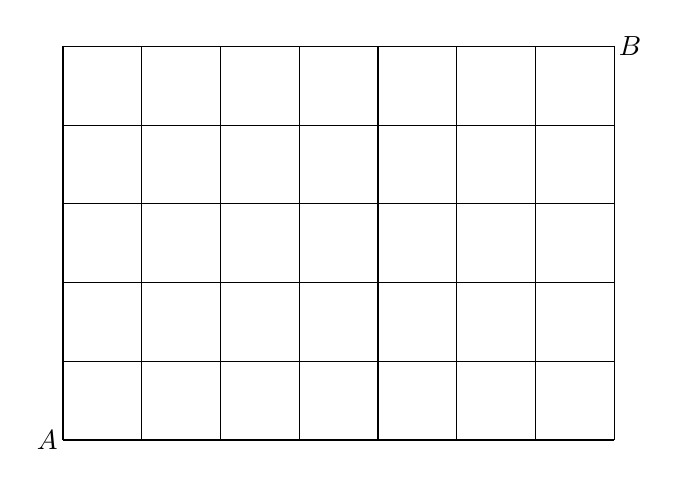
\begin{tikzpicture}
        		\draw (0,0) grid (7,5);
        		\node (a) at (-0.2, 0) {$A$}; 
        		\node (b) at (7.2, 5) {$B$}; 
        \end{tikzpicture}
        \end{center}
		 \end{problem}
		Last time I gave you reasonable grid problems, where you could manually fill out the grid by adding up the number of paths from previous vertices to the next. For this problem, however, the grid seems a little big...
		
		To consider a better way to count the total number of paths, let's just consider a random path that works.
		
		\begin{center}
        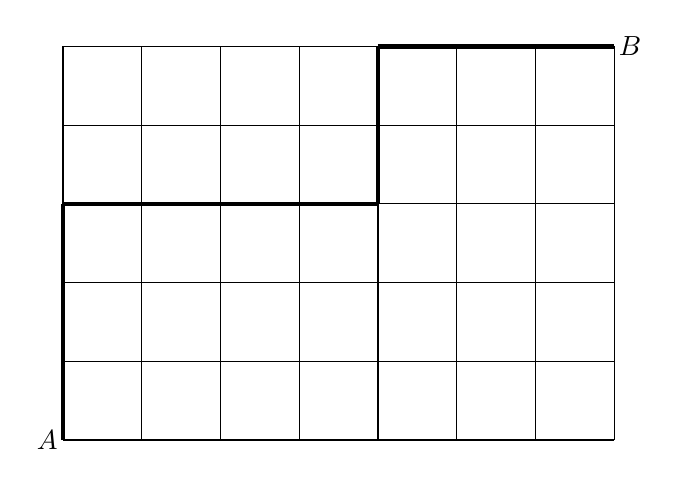
\begin{tikzpicture}
    		\draw (0,0) grid (7,5);
    		\node (a) at (-0.2, 0) {$A$}; 
    		\node (b) at (7.2, 5) {$B$}; 
    		\draw[ultra thick] (0,0) -- (0,3);
    		\draw[ultra thick] (0,3) -- (4,3);
    		\draw[ultra thick] (4,3) -- (4,5);
    		\draw[ultra thick] (4,5) -- (7,5);
        \end{tikzpicture}
        \end{center}
		If we write out the steps to the path above, we get ``UUURRRRUURRR'', where U is ``up'' and R is ``right''. If you play around a bit---in fact, go ahead and draw some paths and write out the steps---you can convince yourself that no matter what your path is, you will end up moving up 5 times and right 7 times. 
		
		Finally, you come to the realization that...``Hey! I just need to count the total number of ways to arrange a word with 5 U's and 7 R's!!!'' And you'd be right, and you'd also be happy to hear you've just derived the formula for finding the number of ways to walk a $m\times n$ grid.
		
		$$\boxed{\text{Number of ways to walk a } m\times n \text{ grid} = \binom{m + n}{n}}$$
		
	\subsection{Paths with Restraints}			
	    Let's begin with a simple problem.

	    \begin{problem}
		 I am currently at home ($A$) and I want to make my way to work at $B$. However, I know there is an accident at point $C$ in the city, so I want to avoid routes that pass through there. Taking this into consideration, how many ways can I drive from $A$ to $B$ if I must not pass through $C$?
		 \begin{center}
        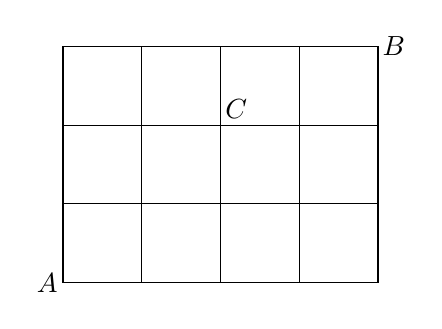
\begin{tikzpicture}
        		\draw (0,0) grid (4,3);
        		\node (a) at (-0.2, 0) {$A$}; 
        		\node (c) at (2.2, 2.2) {$C$};
        		\node (b) at (4.2, 3) {$B$}; 
        \end{tikzpicture}
        \end{center}
		 \end{problem}

		Clearly, it's a lot easier to count the number of paths that go through $C$ rather than the other way around. We can subtract from the total number of paths to get the desired answer for the question.
		
		To solve this problem, all we have to do is break it up into two:
		\begin{enumerate}
		    \item Count the number of ways from $A$ to $C$
		    \item Count the number of ways from $C$ to $B$
		    \item By the fundamental counting principle, the total number of ways will be the product of the two ways above
		\end{enumerate}
        
        So in our case, mirroring the steps above:
        \begin{enumerate}
		    \item Ways from $A$ to $C$: $\binom{4}{2} = 6$
		    \item Ways from $C$ to $B$: $\binom{3}{1} = 3$
		    \item Ways from $A$ to $B$ that go through $C$: $6\times 3 = 18$
		\end{enumerate}
		BUT WAIT, \textbf{WE ARE NOT DONE}!!! The question asked us for the paths that \textbf{don't go through} $C$. So we just subtract from the total:
		$$\binom{7}{3} - 18 = 35-18 = \boxed{17}.$$

    \clearpage
	\subsection{Variations and Disguises}
		Many path counting problems are not just blatantly written out...that would be too easy for you guys and no fun of course. Test writers will often try to hide them to make solving the problem an experience rather than chug and plug. Here we see some typical competition path problems including some infamously difficult ones...
		
		\begin{problem}
		How many ways can I walk from $A$ to $B$ if I am allowed to make two left moves along with the right and up moves I am normally allowed to make?
		\begin{center}
        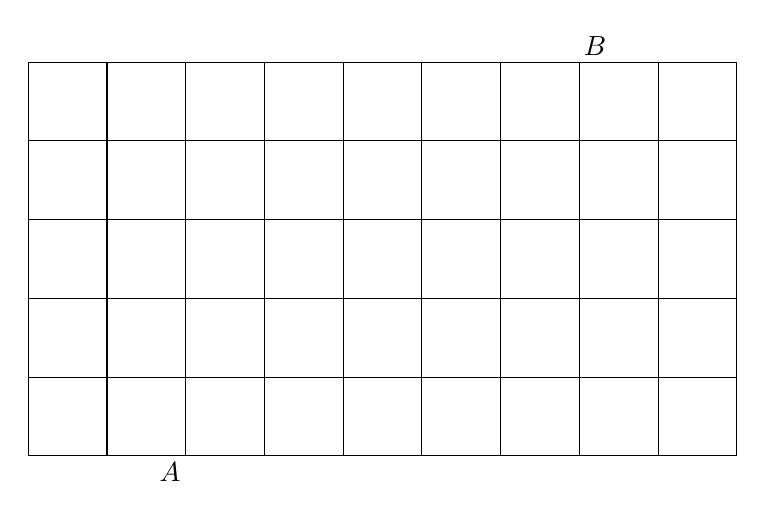
\begin{tikzpicture}
    		\draw (0,0) grid (9,5);
    		\node (a) at (1.8, -0.2) {$A$}; 
    		\node (b) at (7.2, 5.2) {$B$}; 
        \end{tikzpicture}
        \end{center}
        \end{problem}
        
        \begin{problem}
		How many ways can I walk from $A$ to $B$ if I am allowed to make one left move along with the right and up moves I am normally allowed to make? (I am not allowed to walk off the grid!)
		\begin{center}
        \begin{tikzpicture}
    		\draw (0,0) grid (3,2);
    		\node (a) at (-0.2, 0) {$A$}; 
    		\node (b) at (3.2, 2) {$B$}; 
        \end{tikzpicture}
        \end{center}
        \end{problem}
		
		\begin{problem}
		Matt will arrange four identical, dotless dominoes (shaded 1 by 2 rectangles) on the 5 by 4 grid to the right so that a path is formed from the upper left-hand corner A to the lower righthand corner B. In a path, consecutive dominoes must touch at their sides and not just their corners. No domino may be placed diagonally; each domino covers exactly two of the unit squares shown on the grid. One arrangement is shown. How many distinct arrangements are possible, including the one shown? (\textit{Source: MATHCOUNTS State Sprint \#30 2006})
		\begin{center}
        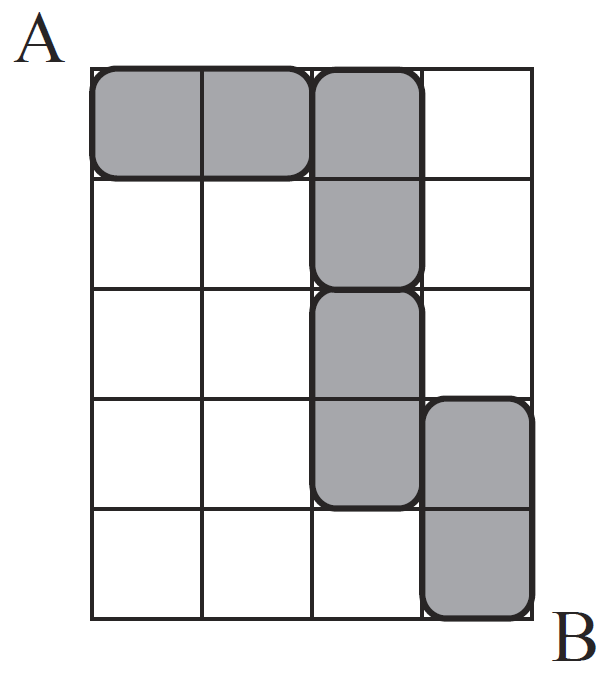
\includegraphics[width=2in]{dominoes}
        \end{center}
		\end{problem}
		
		\clearpage
		
	    \begin{problem}
	    Mack the bug starts at the point (0,0,0) at noon and each minute moves one unit in either the positive $x$-direction, the positive $y$-direction, or the positive $z$-direction. Thus, after 1 minute he could be at (1,0,0), (0,1,0), or (0,0,1). How many different paths could he take to (3,5,2)?
	    \end{problem}

		\begin{problem}
		Cities $A$, $B$, $C$, $D$, and $E$ are connected by roads $\widetilde{AB}$, $\widetilde{AD}$, $\widetilde{AE}$, $\widetilde{BC}$, $\widetilde{BD}$, $\widetilde{CD}$, and $\widetilde{DE}$. How many different routes are there from $A$ to $B$ that use each road exactly once? (Such a route will necessarily visit some cities more than once.)
		\begin{center}
        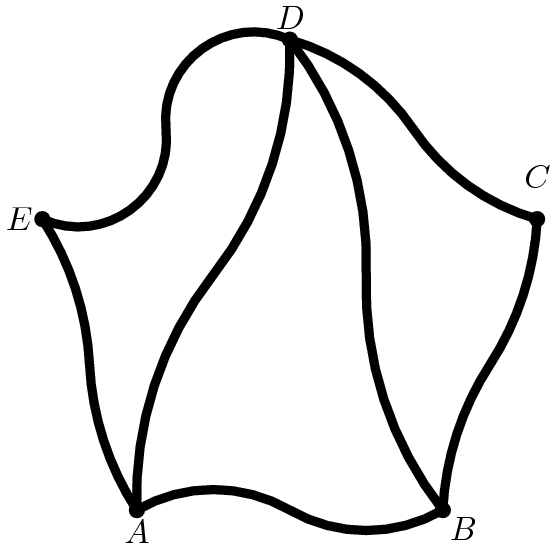
\includegraphics[width=2.5in]{amcgrid}
        \end{center}
		\end{problem}
		
		\begin{problem}
		(\textit{Source: MATHCOUNTS Nationals Sprint \#30})
		\begin{center}
        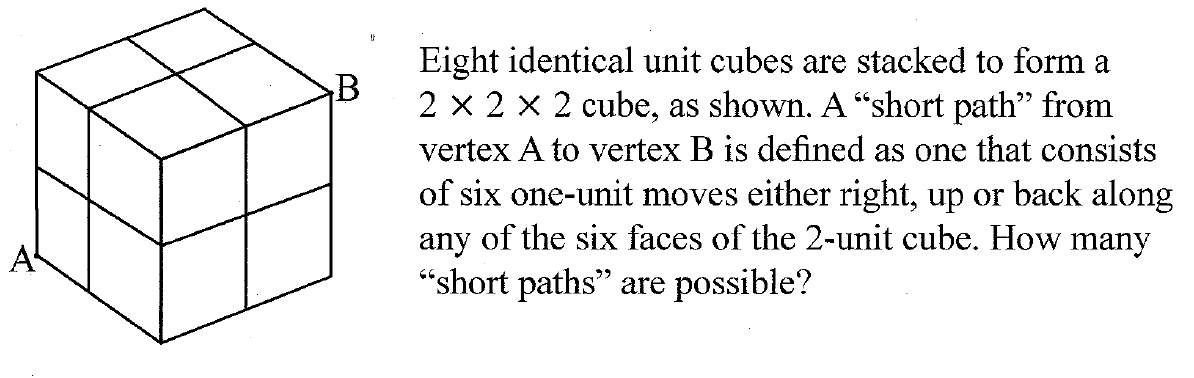
\includegraphics[width=6in]{cube}
        \end{center}
		\end{problem}
		
		\begin{problem}
        In the figure below, how many ways are there to select 5 bricks, one in each row, such that any two bricks in adjacent rows are adjacent? (\textit{HMMT})
        \begin{center}
        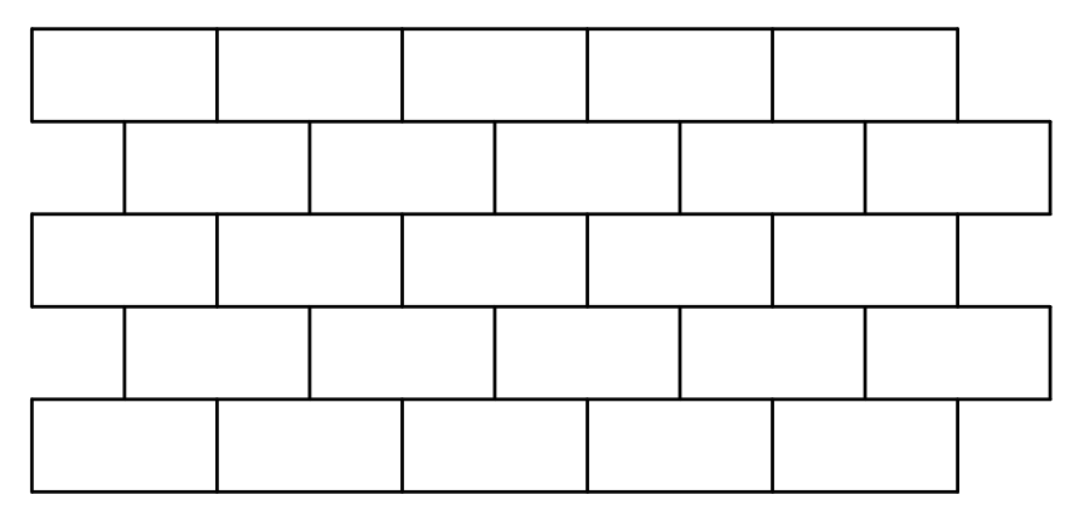
\includegraphics[width=3.5in]{grid}
        \end{center}
        \end{problem}
        
        \clearpage
        
        \begin{problem}
        In the diagram below, how many distinct paths are there from January 1 to December 31, moving from one adjacent dot to the next either to the right, down, or diagonally down to the right? (\textit{HMMT})
        \begin{center}
        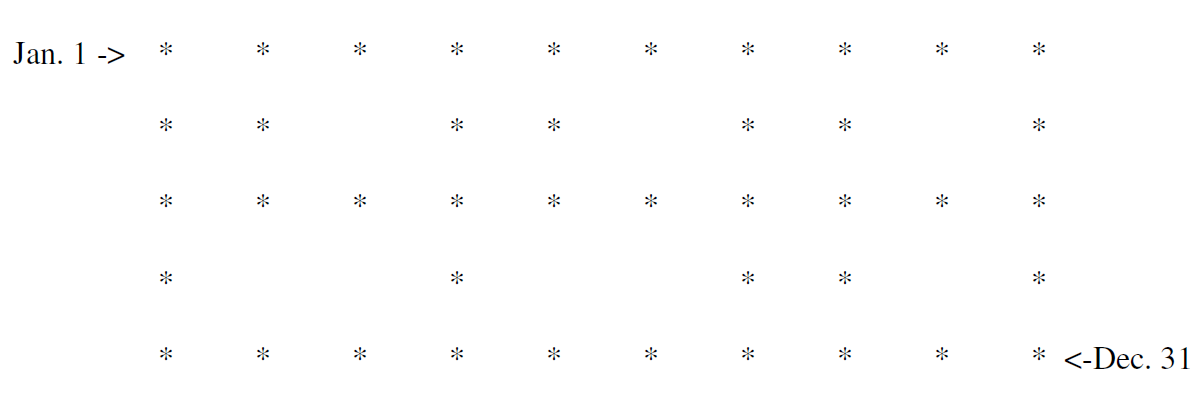
\includegraphics[width=6in]{path2}
        \end{center}
        \end{problem}
		
		\begin{problem}
		A bug travels from A to B along the segments in the hexagonal lattice pictured below. The segments marked with an arrow can be traveled only in the direction of the arrow, and the bug never travels the same segment more than once. How many different paths are there? (\textit{AMC})
        \begin{center}
        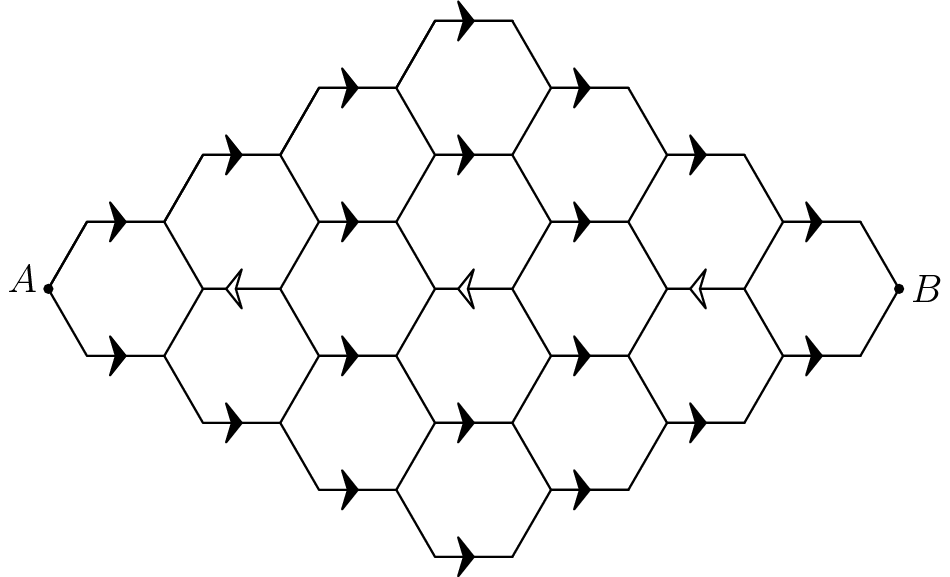
\includegraphics[width=4in]{hexgrid}
        \end{center}
        $\textbf{(A)}\ 2112\qquad\textbf{(B)}\ 2304\qquad\textbf{(C)}\ 2368\qquad\textbf{(D)}\ 2384\qquad\textbf{(E)}\ 2400$
		\end{problem}
		
		\begin{problem}
		I am playing a best-of-three round of rock, paper, scissors with my friend. Since we have played each other a lot, I know the probability that I win any given round is $\frac{2}{3}$, and my friend, $\frac{1}{3}$ (so we never tie). What is the probability I win?
	    \end{problem}
		
		\begin{problem}
		The Patriots and the Seahawks are going to fight a tough game tonight. Due to poor score tracking technology, the two teams can only score with touchdowns (and no extra points), so 6 points whenever a team scores. One analyst predicts the score will be 36-30, with the Patriots winning and never trailing the Seahawks. Another analyst predicts the score will be 42-24, with the Seahawks routing the Patriots, except this time the Seahawks never trail nor tie with the Patriots. How many ways can each of the scenarios happen, and what are their probabilities?
		\end{problem}
		
		\begin{problem}
		The Boston Red Sox and New York Yankees are playing a best of 7 at the World Series. It is well known that for any game, the Yankees have a $\frac{3}{5}$ chance of winning and the Red Sox have a $\frac{2}{5}$ chance of winning. With this knowledge, what is the probability that the teams will go to a game 7?
		\end{problem}
\newpage
\section{Sticks and Stones}
\subsection{Distributing Candy to Kids}

Suppose we have this problem, 

\begin{problem}
I have 10 identical pieces of candy. In how many different ways can I distribute the candies to 5 different kids?
\end{problem}

At first it seems really difficult, right? I could give out $(2, 2, 2, 2, 2)$, $(1, 2, 3, 4, 0)$, $(0, 0, 10, 0, 0)$, etc...the list doesn't seem to end. 

The strategy we're going to employ right now is called \textit{using simplifications to find generalizations}. The tip doesn't sound very useful, so hopefully this solution can help. We will begin by assuming we have 1 piece of candy and $m$ number of kids.

\begin{itemize}
    \item Suppose we only had \textbf{1 piece of candy}. Now it's pretty easy right? We can only give this piece of candy to one of the $m$ kids, so we have $\boxed{m}$ ways when there is 1 piece of candy. 
    \item \textbf{2 pieces}. We can either give 2 to one kid, or 1 to two kids. We have a total of $$\boxed{\binom{m}{1}+\binom{m}{2}}.$$
    \item \textbf{3 pieces}. We can still manage, this...we can do either 3 all to one kid, 2 to one kid and 1 to another, or 1 to three kids. This gives us $\boxed{\binom{m}{1}+\binom{m}{2}+\binom{m}{3}}$
\end{itemize}

we found some stuff, but the casework is looking very ugly, how about let's reduce the number of kids instead? (and generalize to $n$ pieces of candy as well)

\begin{itemize}
    \item Suppose we only had \textbf{1 kid}. Then we can only give out the candy $\boxed{1}$ way
    \item \textbf{2 kids}. We can give the first kid $0, 1, \cdots, n$, and give the second kid the rest. There are $\boxed{n+1}$ ways
    \item \textbf{3 kids}. Hm...it's starting to get hard but we can still manage with case work. We can give 0 to the first kid, and have the 2 kid problem again, giving $n+1$, give 1 to the first kid, and have $n$ choices for the other two kids, and so on, giving $(n+1)+n+(n-1)+\cdots+1 = \boxed{\frac{(n+1)(n+2)}{2}}$ 
\end{itemize}

Yikes...it looks messy for both but at least we've made some progress.

\subsubsection{Organize Your Progress}
Maybe we can try to summarize what we've done by making a chart of the total number of ways to distribute $m$ candies to $n$ children,


\begin{table}[H]
    \centering
    \begin{tabular}{cc|cccccc}
 && \multicolumn{5}{c}{Kids} \\
 && 1 & 2&3&4&5&6 \\
 \hline
 \hline
 & 0&1&1&1&1&1&1\\
  & 1& 1&2 &3&4&5&6\\
 \parbox[t]{2mm}{\multirow{3}{*}{\rotatebox{90}{Candy}}}& 2 &1&3&6&10&15&21\\
 & 3 &1&4&10&20&35&56\\
 & 4 &1&5&15&35&70&126 \\
 & 5 &1&6&21&56&126&252
    \end{tabular}
    \label{tab:candy}
\end{table}

Hmm....where have we seen these numbers before?

Perhaps you recall \textbf{Pascal's Triangle}:

\begin{center}
\begin{tabular}{ccccccccccccc}
 &&&&&1&&&&&&&\\
 &&&&1&&1&&&&&\\
 &&&1&&2&&1&&&\\
 &&1&&3&&3&&1&\\
 &1&&4&&6&&4&&1\\
\end{tabular}
\end{center}

Let's replace the numbers in our table with combinations $\binom{n}{r}$ to maybe see if we can discover a simple solution to our problem.


\begingroup
\setlength{\tabcolsep}{6pt} % Default value: 6pt
\renewcommand{\arraystretch}{1.5} % Default value: 1
\begin{table}[H]
    \centering
    \begin{tabular}{cc|CCCCCC}
 && \multicolumn{5}{c}{Kids} \\
 &&  1& 2&3&4&5&6 \\
 \hline
 \hline
 &0 &\binom{0}{0}&\binom{1}{1}&\binom{2}{2}&\binom{3}{3}&\binom{4}{4}&\binom{5}{5}\\
 &1&\binom{1}{0}& \binom{2}{1} &\binom{3}{2}&\binom{4}{3}&\binom{5}{4}&\binom{6}{5}\\
 \parbox[t]{2mm}{\multirow{3}{*}{\rotatebox{90}{Candy}}}& 
 2 &\binom{2}{0}&\binom{3}{1}&\binom{4}{2}&\binom{5}{3}&\binom{6}{4}&\binom{7}{5}\\
 &3&\binom{3}{0}&\binom{4}{1}&\binom{5}{2}&\binom{6}{3}&\binom{7}{4}&\binom{8}{5}\\
 &4&\binom{4}{0}&\binom{5}{1}&\binom{6}{2}&\binom{7}{3}&\binom{8}{4}&\binom{9}{5} \\
 &5&\binom{5}{0}&\binom{6}{1}&\binom{7}{2}&\binom{8}{3}&\binom{9}{4}&\binom{10}{5}
    \end{tabular}
    \label{tab:candy2}
\end{table}
\endgroup

There seems to be some sort of pattern...every time the number of pieces of candy goes up by 1, $\binom{n}{r}$ goes to $\binom{n+1}{r}$, and when the number of kids goes up, $\binom{n+1}{r+1}$. Testing formulas, we can reason that 

$$\boxed{\text{Number of ways to distribute } r \text{ candies to } n \text{ kids} = \binom{n+r-1}{n-1}}.$$

Finally, we can solve our problem! We have $n = 5 \text{ kids}, r = 10 \text{ candies}$, so 

$$\binom{k+n-1}{n-1} = \binom{10+5-1}{5-1} = \binom{14}{4} = \boxed{1001}.$$

Imagine doing the casework to get 1001 as your answer...yikes.

\subsubsection{Another Perspective}

It seems like even though we found a simple solution to our answer, there was a \textit{lot} of work that we had to do in order to get to our result. Furthermore, our proof (which I didn't present formally) was basically a pattern identification one. There must be a better way to do this problem, right?

And of course, there is a better way to do this. Suppose that we put all 10 candies on a table and put 4 dividers to represent how much candy each person gets. For example, 

$$\bu |\bu |\bu \bu \bu |\bu \bu \bu |\bu \bu,$$

would represent the distribution $(1, 1, 3, 3, 2)$. For you skeptical folks, you might claim this method doesn't always work, suppose we have 

$$\bu ||\bu \bu \bu \bu \bu \bu \bu ||\bu \bu.$$

What do we do now? There are dividers next to each other...but then we realize that we're allowed to give children 0 pieces of candy, so this case just represents $(1, 0, 7, 0, 2)$.

Now the problem is easy right? All we have to do is arrange 4 $|$ and 10 $\bu$, which is the same as $\boxed{\binom{14}{4}}$, the answer we got earlier. Now, it's clear why there's a minus one in our formula for the total number of ways to distribute candies---we only need $n-1$ dividers for $n$ children. When we have an argument like this---that we can find another problem that solves the problem we are trying to do---we are making a \textbf{bijection}, also known as a one-to-one correspondence. Bijections are powerful in problem-solving because as you can see in this problem, you can find a correspondence that is much easier to solve than the original.

\subsection{The Hockey Stick Identity}

Suppose we have the problem (yes, these problems really do show up in competition math):

\begin{problem}
Compute 
$$\binom{4}{4}+\binom{5}{4}+\cdots+\binom{12}{4}$$
\end{problem}

There are two ways to approach this problem. We just did a long problem about distributing $r$ candies to $n$ kids, and if we look carefully, the sum is asking for

$$P(0,5)+P(1,5)+\cdots+P(8,5),$$

where $P(r,n)$ is a function that describes the number of ways to distribute $r$ candies to $n$ kids. Of course, from our casework earlier, we recognize this sum as $N(8,6)$, because it's the casework we would do if we gave one of the kids $0,1,\cdots,8$ pieces of candy and redistributed the rest to the others. Therefore, our answer is $N(8,6) = \boxed{\binom{13}{5}}$.

Hmm...our answer does look suspicious, but maybe it'll be clearer if we try our second method, which if you haven't guessed already, is using Pascal's Triangle. For the sake of saving paper and not drawing a huge triangle, let's instead calculate 

$$\binom{1}{1}+\binom{2}{1}+\binom{3}{1}.$$
\clearpage

I know the problem is really easy, but let's draw our handy dandy Pascal's Triangle:

\begingroup
\setlength{\tabcolsep}{3pt} % Default value: 6pt
\renewcommand{\arraystretch}{1.5} % Default value: 1
\begin{center}
\begin{tabular}{CCCCCCCCC}
     &&&&\binom{0}{0}&&&& \\
     &&&\binom{1}{0}&&\binom{1}{1}&&& \\
     &&\binom{2}{0}&&\binom{2}{1}&&\binom{2}{2}&& \\
     &\binom{3}{0}&&\binom{3}{1}&&\binom{3}{2}&&\binom{3}{3}& \\
     \binom{4}{0}&&\binom{4}{1}&&\binom{4}{2}&&\binom{4}{3}&&\binom{4}{4} \\
\end{tabular}
\end{center}
\endgroup

If you follow the path of $\binom{1}{1}+\binom{2}{1}+\binom{3}{1}$ and veer right, you end up at $\binom{4}{2}=6$, which happens to our answer. This property seems peculiar, that the sum of the elements along a diagonal add up to the element below and to the right of the last. But this in fact is \textit{always} true, and because the shape that we draw on Pascal's Triangle is supposed to remind you of a hockey stick, we call it the \textbf{Hockey Stick Identity}. Formally, the theorem states

$$\boxed{\binom{r}{r}+\binom{r+1}{r}+
\cdots+\binom{n}{r}=\binom{n+1}{r+1}, r\geq 0, n\geq r}.$$

Now, to prove this theorem the non-Pascal's triangle and non-counting way, we turn to our most reliable friend, algebra. We have

$$\binom{r}{r}+\binom{r+1}{r}+\cdots+\binom{n}{r}.$$

Of course, if you recall last week's lecture, it seems like Pascal's is just \textit{dying} to have us use his identity, 

$$\binom{n}{r}+\binom{n}{r+1}=\binom{n+1}{r+1}.$$

Of course, the terms in our sum don't have the same top component of the combination, so it seems like we are stuck. But wait! $\binom{r}{r}=1=\binom{k}{k},\forall k\in \mathbb{Z}$, we can just change our first term to $\binom{r+1}{r+1}$ and apply Pascal's to the first two terms,

\begin{align*}
    \binom{r+1}{r+1}+\binom{r+1}{r}+\binom{r+2}{r}+\binom{r+3}{r}+\cdots&=\binom{r+1}{r+1}+\binom{r+2}{r}+\binom{r+3}{r}+\cdots \\
        &=\binom{r+2}{r+1}+\binom{r+3}{r}+\cdots \\
        &=\binom{r+3}{r+1}+\cdots
\end{align*}

and you should get the idea. When we get to the last two terms, we have 

$$\binom{n}{r+1}+\binom{n}{r}=\binom{n+1}{r+1},$$

which is just Pascal's identity, and we have proved our theorem. We call this technique \textbf{telescoping}, when we are able to ``shrink'' our expression.

\clearpage

\subsection{Problems}
\begin{problem}
Find the total number of ways to distribute:
\begin{itemize}
    \item 9 candies to 5 children
    \item 4 candies to 7 children
    \item 14 candies to 5 children if each child must receive \textit{at least} 1 piece
    \item 17 pieces of candy to 5 kids, if the youngest kid can't get more than any of the others
\end{itemize}
\end{problem}

\begin{problem}
How many ways can I distribute 8 LEGO sets, 5 Hot Wheels cars, 7 video games, and 10 Pok\'{e}mon cards to 4 children if each child has to receive at least one of each type of toy?
\end{problem}

\begin{problem}
Alice, Bob, Charlie, and Dave are running for President of their class. There are 100 people voting in this election. How many outcomes are possible if (you can leave your answer unsimplified):
\begin{enumerate}[label=(\alph*)]
    \item Everybody votes?
    \item Some people abstain (don't vote)?
\end{enumerate}
\end{problem}

\begin{problem}
Compute 
$$\binom{2}{2}+\binom{3}{2}+\cdots+\binom{16}{2}$$
\end{problem}

\begin{problem}
Compute 
$$\binom{7}{3}+\binom{8}{3}+\cdots+\binom{14}{3}$$
\end{problem}

\begin{problem}
Compute
$$12\binom{3}{3}+11\binom{4}{3}+\cdots+2\binom{13}{3}+\binom{14}{3}$$
\end{problem}

\begin{problem}
When $(x+y+z)^{2009}$ is expanded and like terms are grouped together, there are $k$ terms with coefficients that are \textit{not} multiples of 5. Find $k$. \textit{Hint: Write 2009 in base 5}

\textit{Source: TJ ARML Practice}
\end{problem} 

\begin{problem}
The polynomial $1-x+x^2-x^3+\cdots+x^{16}-x^{17}$ may be written in the form $a_0+a_1y+a_2y^2+\cdots +a_{16}y^{16}+a_{17}y^{17}$, where $y=x+1$ and the $a_i$'s are constants. Find the value of $a_2$. \textit{Source: AIME}
\end{problem}

\begin{problem}
Consider all 1000-element subsets of the set {1, 2, 3, ... , 2015}. From each such subset choose the least element. The arithmetic mean of all of these least elements is $\frac{p}{q}$, where $p$ and $q$ are relatively prime positive integers. Find $p + q$. \textit{Source: AIME}
\label{p1}
\end{problem}

\begin{problem}
The Annual Interplanetary Mathematics Examination (AIME) is written by a committee of five Martians, five Venusians, and five Earthlings. At meetings, committee members sit at a round table with chairs numbered from $1$ to $15$ in clockwise order. Committee rules state that a Martian must occupy chair $1$ and an Earthling must occupy chair $15$, Furthermore, no Earthling can sit immediately to the left of a Martian, no Martian can sit immediately to the left of a Venusian, and no Venusian can sit immediately to the left of an Earthling. The number of possible seating arrangements for the committee is $N(5!)^3$. Find $N$. \textit{Source: AIME}
\end{problem}

\begin{problem}
Let $1 \le r \le n$ and consider all subsets of $r$ elements of the set $\{ 1, 2, \ldots , n \}$. Each of these subsets has a smallest member. Let $F(n,r)$ denote the arithmetic mean of these smallest numbers; prove that

$$F(n,r) = \frac{n+1}{r+1}.$$

\textit{Source: IMO}
\end{problem}
\newpage
\section{Recursion}
Although the idea of recursion is simple---it's something that calls on itself---understanding it can be kind of tricky. For example, to start off with a simple example, consider the following joke:
\begin{center}
\textit{``Q: What is Benoit B. Mandelbrot's middle name? A: Benoit B. Mandelbrot.''}
\end{center}
Recursion gets complicated because we relate unknowns with...more unknowns. Although this seems to make problems more complex than they actually are, it actually gives us beautiful and simple relationships.

\subsection{Fibonacci}
Perhaps the most famous recursion is the \textbf{Fibonacci Sequence}, which is defined by the following, 

\begin{equation}
    F_n = F_{n-1} + F_{n-2},\!\, 
\end{equation}
where starting values are $F_1=F_2=1$.

If you plug into the formula, starting with computing $F_3 = F_2+F_1 = 1+1 =2$, you can compute the first few terms,

$$ 1,\;1,\;2,\;3,\;5,\;8,\;13,\;21,\;34,\;55,\;89,\;144,\; \ldots\; $$

\subsubsection{Fibonacci in Disguise}
It turns out that understanding simple recurrence relationships like Fibonacci can help us solve a host of problems. 

\begin{ex}
Lou is climbing a  flight of 4 stairs.  With each step, he will climb either 1 or 2 stairs.
In how many different ways can he climb the flight of stairs?
\end{ex}

\begin{ex}
In how many ways can we tile a $2\times9$ checkerboard with tiles of size $2\times 1$, such that each tile covers exactly two squares? (no overlapping tiles)
\end{ex}

\subsection{Classic Recursion}
This section will present more typical examples for you to familiarize yourself with the recursion process. Remember, finding a \textbf{recurrence relation} is what allows us to make these problems easier to count---you break the problem into smaller parts that build on each other.

\begin{ex}
Find the number of 8-digit sequences that only have 0,1,2, but no two consecutive zeros.
\end{ex}

\begin{ex}
There are 12 spaces in a parking lot, and today I know I will be expecting Porsches, which take up 1 space, Jeeps and Cadillacs, which both take 2 spaces each, and Jeeps, Hummers, and Trucks, which each take up 3 spaces each. How many ways can these cars (which there are infinite number of) fill up the 12 spaces in the parking lot?
\end{ex}

\subsubsection{Linear Recurrences}
Suppose we had some recurrence relation 

\begin{equation}
    a_n = c_{n-1}a_{n-1}+c_{n-2}a_{n-2}+\cdots+c_0a_0,
\end{equation}
where $a_i$ is a term in the sequence $\{a_i\}_{i=1}^{N}$, and $c_i$ is some function (it's usually a constant for our purposes). Then our question is, \textit{can we find a closed form for $a_n$}?

At first, you might say, why would I bother wanting to find a closed form? Well try this problem,

\begin{ex}
You are trying to stack a tower that is 100 ft tall. You have 5 colors of 1 ft tall blocks and 6 colors of 2 ft tall blocks. How many distinct towers can you construct? (you have infinite number of each block)
\label{ex:lr}
\end{ex}

The recurrence relation is easy, you can either use one of 5 kinds of 1 ft tall blocks, which leaves you with finding $a_{n-1}$ ways to stack, or use one of 6 kinds of 2 ft tall blocks, which leaves you with finding $a_{n-2}$ ways to stack. Thus, the recurrence relation is
\begin{equation}
    a_n = 5a_{n-1}+6a_{n-2}.
\end{equation}

And you could start computing some values for $a_n$, 

\begin{table}[H]
    \centering
    \begin{tabular}{c|c}
        $n$ & $a_n$\\
        \hline
         1 & 5 \\
         2 & 31 \\
         3 & 185 \\
         4 & 1111 \\
         \multicolumn{2}{c}{
         $\cdots$}
    \end{tabular}
    \caption{Some values for $a_n$}
    \label{tab:my_label}
\end{table}
but quickly, you see that the values are getting out of hand...

Therefore, our motivation for finding a general formula is not just for the pure mathematics fun, but also so it can make our calculations easier. 

To do a linear recurrence, we use the fact that, well, the recurrence relation is \textbf{linear}. As pre-high school students (or pre-linear algebra students), however, you probably have \textit{no idea} what I mean by a linear property. 

\begin{theorem}
A function $f(x)$ is said to be linear if it satisfies:
\begin{itemize}
    \item \textbf{Additivity:} $f(x+y) = f(x)+f(y)$
    \item \textbf{Homogeneity:} $f(kx) = kf(x)$
\end{itemize}
\end{theorem}

We'll need a little more to understand more to get to our next results, but for our purposes, we're only interested in solving the problem. If you really want some insight into it, you can think of a linear function as a matrix multiplication. Try to absorb this next theorem.

\begin{theorem}
Assuming that  
\begin{equation*}
    a_n = \sum\limits_{k=1}^{n-1} c_{k}a_{k}
\end{equation*}
can be written as a linear recurrence, we know the solutions are in the form
$$a_n = \sum\limits_{k=0}^{r} \lambda_k p^n,$$
where $p$ is some unknown constant that is solved for by substituting $a_n = p^n$
\label{thm:2}
\end{theorem}

Using Theorem \ref{thm:2}, we can now solve our linear recurrence in Example \ref{ex:lr}. We have 

\begin{align*}
    a_n &= 5a_{n-1}+6a_{n-2} \\
    p^n &= 5p^{n-`}+6p^{n-2} 
\end{align*}
Dividing the equation through by $p^{n-2}$ yields us a quadratic
\begin{align*}
    p^2-5p-6 &= 0 \\
    (p-6)(p+1) &= 0 
\end{align*}
which yields the roots $p=-1, 6$. It is important to note that the quadratic we got here is known as the \textbf{characteristic polynomial}; this implies in general, of course, that it won't necessarily be a quadratic. With these roots, we now know our solutions are in the form
\begin{equation}
    a_n = \lambda_1 (-1)^n + \lambda_2 (6)^n.
\end{equation}
How do we find our two unknown constants? Well it's actually really easy. We just need to plug in two values of $a_n$, giving us a system. To make our lives easier, we'll just use $a_1, a_2$:
\begin{align*}
    a_1 &= -\lambda_1+6\lambda_2 = 5\\
    a_2 &= \lambda_1+36\lambda_2 = 31.
\end{align*}
This system yields $(\lambda_1, \lambda_2) = (\frac{1}{7},\frac{6}{7})$. We finally have our answer, which looks very clean now
\begin{equation}
    \boxed{a_n = \frac{1}{7}(-1)^n+\frac{6}{7}(6)^n}
\end{equation}
If you're skeptical of this answer, try plugging in $n-3, 4$, and seeing if it matches up with what we got earlier.

\subsubsection{Degenerate Linear Recurrences}
Suppose our linear recurrence is 
\begin{equation}
    a_n = 4a_{n-1}-4a_{n-2}.
\end{equation}
We can easily find our roots $p$ with the characteristic polynomial,
\begin{equation}
    p^2-4p+4 = 0,
\end{equation}
which gives us the roots $p=2$...that is a double root at $p=2$. We are sort of stuck here, because we have no idea what to do now that we have a repeated root. There are ways to prove this next theorem, but we'll just have to take it for fact now since it requires linear algebra arguments.

\begin{theorem}
If $p_0$ is a root of the characteristic polynomial $C(p)$ with multiplicity $r$ (repeated $r$ times), then the $p_0$ contribution to the general solution $a_n$ will be
\begin{equation}
    \sum\limits_{k=0}^{r-1} (n)^{k} \lambda_k (p_0)^n = (p_0)^n\left(\lambda_0 + \lambda_1 n +\lambda_2 n^2 + \cdots +\lambda_{r-1} n^{r-1}\right)
\end{equation}
\label{thm:deg}
\end{theorem}

Using Theorem \ref{thm:deg}, we know our general solution will be in the form 
\begin{equation}
    a_n = \lambda_0 (2)^n + n\lambda_1 (2)^n.
\end{equation}
Now we can solve for the constants given initial conditions just like we did with the earlier example.

\subsection{Recursive Functions}
Suppose you had to evaluate
\begin{equation}
    \frac{1}{1+\frac{1}{1+\frac{1}{1+\cdots}}}
\end{equation}

Of course, thinking like a mathematician, you turn to trying small cases and trying to induct on them. We compute the following:

\begin{itemize}
    \item $\frac{1}{1} = 1$
    \item $\frac{1}{1+\frac{1}{1}} = \frac{1}{2}$
    \item $\frac{1}{1+\frac{1}{1+\frac{1}{1}}} = \frac{2}{3}$
    \item $\frac{1}{1+\frac{1}{1+\frac{1}{1+\frac{1}{1}}}} = \frac{3}{5}$
    \item $\frac{1}{1+\frac{1}{1+\frac{1}{1+\frac{1}{1+\frac{1}{1}}}}} = \frac{5}{8}$
\end{itemize}

Hm...where have we seen the numbers in these fractions? Maybe you recall the Fibonacci sequence again! Let's try to prove why this is true. 

\begin{lemma}
Each term in the sequence $\{a_i\}_{i=1}^{\infty}$ has the form
\begin{equation}
    a_n = \frac{F_{n}}{F_{n+1}},
\end{equation}
where $F_n$ is the $n^{\text{th}}$ term of the Fibonacci sequence.
\label{lm:1}
\end{lemma}

\textit{Proof.} We proceed with this proof by induction. For $n=1$, the lemma clearly holds, as
$$a_1 = \frac{1}{1}= \frac{F_1}{F_2}.$$
For a general $n$, we can find the next term by the following relationship of the sequence $a_i$, derived from the original continued fraction relationship.
\begin{equation}
    a_{n+1} = \frac{1}{1+a_{n}}
    \label{eq:lm1}
\end{equation}
So now using Equation (\ref{eq:lm1}), we can find $a_{n+1}$, 

\begin{align*}
    a_{n+1} &= \frac{1}{1+a_{n}} \\
            &= \frac{1}{1+\frac{F_n}{F_{n+1}}} \\
            &= \frac{F_{n+1}}{F_{n+1}+F_{n}} \\
            &= \frac{F_{n+1}}{F_{n+2}} 
\end{align*}
which completes the induction. $\Box$

From Lemma \ref{lm:1}, we can compute the value for the infinitely continued fraction. Since the closed form of Fibonacci can be written as the following, where $\varphi = \frac{1+\sqrt{5}}{2}$ (the golden ratio),
\begin{equation}
    F\left(n\right) = \frac{\varphi^n-(-\varphi)^{-n}}{\sqrt{5}},
\end{equation}
we can easily compute what the expression should equal. 
\begin{align*}
    x &= \lim_{n\to\infty} \frac{F_n}{F_{n+1}}\\
      &= \lim_{n\to\infty} \frac{\frac{\varphi^n-(-\varphi)^{-n}}{\sqrt{5}}}{\frac{\varphi^{n+1}-(-\varphi)^{-(n+1)}}{\sqrt{5}}} \\
      &= \boxed{\frac{1}{\varphi}}.
\end{align*}

Instead of using the first method, let's think of this problem in another recursive perspective. Suppose we assumed the value of the continued fraction to a value, let's call it $x$, 

\begin{equation}
    x = \frac{1}{1+\frac{1}{1+\frac{1}{1+\cdots}}}.
\end{equation}

Then aha! We see something. Inside the fraction, we can find $x$ again. Namely, we can substitute $x$ where it appears again, giving:

\begin{align*}
    x &= \frac{1}{1+x} \\
    x^2 + x -1 &= 0, \quad x = \boxed{\frac{-1+\sqrt{5}}{2}},
\end{align*}
which is the same answer that we got earlier. Notice that we take the positive root of the quadratic since the original expression is clearly positive. When you have to evaluate recursive expressions like this continued fractions example, it is almost always easier to use the algebraic method.



\subsection{Problems}
\begin{problem}
Your Pok\'{e}mon has 10 PP left (this is different from the normal game where you have PP for each move. Your moves are tackle and weaken (1 PP), tail whip (2 PP),  and thunderbolt (3 PP). How many distinct sequences of moves can you make that uses up all 10 of your PP?
\end{problem}

\begin{problem}You are part of the biotech lab, and need to produce enough goats for your fantastic experiment. However, you only have 2 adult goats, which can produce 4 baby goats every month. Fortunately, these goats are super goats that never die, and their babies are also super goats. In addition, these super goat babies only take a month to reach adulthood and have the ability to reproduce more baby goats. You need 337 goats by the end of five months---will your super goats be able to do it?
\end{problem}
\begin{problem} It is well known that listening to Lil-Wayne, Nicki Minaj and Justin Bieber causes an extraordinary amount of auditory damage. Therefore, you must rest for at least one hour after listening to an entire album by Justin Bieber, two for Nicki Minaj, and three for Lil-Wayne, before listening to any more music. With that in mind, and the fact that all albums in this problem are an hour long, how many distinct 6-hour playlists can you create with unlimited of one unique Taylor Swift (no rest needed), 9 Justin Bieber (1 hr rest), 11 Nicki Minaj (2 hr rest), and 4 Lil-Wayne (3 hr rest) albums? \textit{Extension: How about for a 12-hour playlist? Use linear recurrences!}
\end{problem}
\begin{problem}Beyonc\'{e} and Jay Z are bored out of their minds after they retire, and decide to play a Grammy trading game. Each one of them puts 14 Grammys on the table. The rules are as follows: each turn, a coin is flipped. If it is heads Beyonc\'{e} gets to take a Grammy from Jay Z, and if it is tails, Jay Z takes it from Beyonc\'{e}. Now Jay Z, being a math champ, is saying ``naw this game is too boring and we are equally likely to win''. Beyonc\'{e}, on the other hand, replies by saying that whoever ends up with all 28 Grammys on the table gets to take it, making the game more interesting. What is the expected number of turns it takes for either one of them to win the Grammy game?
\end{problem}

\begin{problem} The Boston Celtics and the Los Angeles Lakers meet for their \nth{95} NBA final in the year 2318. The series is hard fought, and after six games, you want to compute the probability that the teams are tied three games apiece. Given that the Celtics win any game with probability $\frac{3}{5}$ and the Lakers win any game with probability $\frac{2}{5}$, what is this probability?
\end{problem}
\begin{problem}Michael Phelps is training for the 2016 Rio Olympics. Unfortunately, because he has been enjoying life and slacking off in practice, he is extremely out of shape. Today, during practice, his coach decides that Michael will not leave the pool unless he finishes 5 sets of 400 IM consecutively on an interval of 4:30. Phelps, with all the time he's been slacking, gives up on a 400 IM with probability $\frac{1}{5}$ every time, which means he will have to start over the entire set (that's 5 more 400 IMs Mike...good luck dying). What is the expected number of times he will have to swim the 400 IM before he drags himself out of the pool?
\end{problem}

\begin{problem}
Solve for $x$, where
\begin{equation}
    x = \sqrt{x+\sqrt{x+\sqrt{x+\cdots}}}
\end{equation}
\end{problem}

\chapter{Geometry}
\section{Triangles}
Triangles are the fundamental shapes that make up (literally) much of geometry. The purpose of this lecture is not to provide a rigorous, in-depth treatment of geometry, but rather give formulas and definitions that will aid a student in solving competition math problems. Keep in mind that the material in this lecture ranges from introductory to intermediate, so it covers a wide range of difficulties. This lecture is partly adpated from Jennifer Yin's ``Triangles!'' lecture from TJ VMT ARML practice on March 7, 2013.
\subsection{Special Properties of Triangles}
There are lines and points on triangles that have special properties:
\begin{enumerate}
    \item \textbf{Medians:} These intersect the sides of a triangle at their midpoints; their common point of intersection is called the \textbf{centroid}. An important property of medians is that the length of a centroid to a vertex is always twice that of its distance to the opposite side.
    \item \textbf{Angle Bisectors:} These are the lines of a triangle that bisect the angles of a triangle. The angle bisectors of a triangle intersect at a common point called the triangle's \textbf{incenter}, which is the center of the triangle's \textbf{incircle} (a circle that can be inscribed inside the triangle that is tangent to all three sides).
    \item \textbf{Perpendicular Bisectors:} These lines perpendicularly bisect the sides of the triangle. Their common point of intersection is called the \textbf{circumcenter}, which is the center of the triangle's \textbf{circumcircle}.
    \item \textbf{Altitudes:} These intersect at a common point called the triangle's \textbf{orthocenter}. Problems that involve altitudes typically use the Pythagorean theorem.
\end{enumerate}

\clearpage
\subsection{Formulas for the Triangle}
All of these theorems have proofs that you can look up. Some are easy to prove, but others can be very difficult. Although it's important to understand how some of them are derived, it is not necessary to know them in order to solve problems.
\subsubsection{Side Lengths}
\begin{itemize}
    \item \textbf{Pythagorean Theorem:} $\displaystyle a^2+b^2=c^2$, where $c$ is the hypotenuse and $a, b$ are the two legs of a \textit{right triangle}. Arguably one of the most basic and important equations you'll need to know.
    \item \textbf{Angle Bisector Theorem:} If $\bigtriangleup ABC$ has an angle bisector from $A$ that intersects $BC$ at  $D$, then $\displaystyle \frac{AB}{BC} = \frac{AC}{CD}$ 
    \item \textbf{Law of Cosines: } $\displaystyle c^2 = a^2+b^2-2ab\cos\theta$, where $\theta=\angle ACB$ (the angle at $C$).
    \item \textbf{The Law of Sines: } $\displaystyle \frac{a}{\sin A} = \frac{b}{\sin B} = \frac{c}{\sin C} = 2R$, where $a$ denotes side $BC$ and $A$ denotes the angle at $A$.
    \item \textbf{Stewart's Theorem:} $b^2m + c^2n = a(d^2 + mn)$ This theorem works for any cevian $AD$ of $\bigtriangleup ABC$. This theorem is better remembered as $dad+man=bmb+cnc$, which (if you use your imagination), can be read as ``Dad and man put a bomb in the sink.''
    \begin{center}
    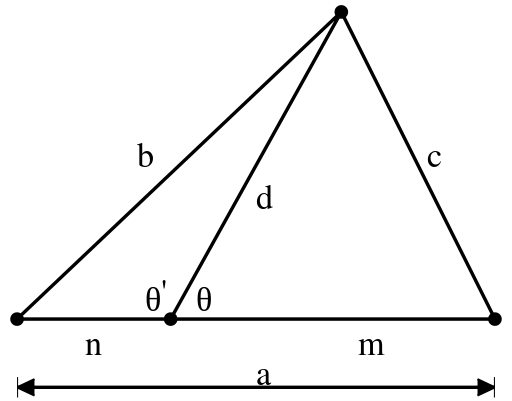
\includegraphics[width = 2in]{stewarts}
    \end{center}
    \item \textbf{Ceva's Theorem:} $\frac{AF}{AE} = \frac{BD}{BF} = \frac{CE}{CD} = 1$, where $\bigtriangleup ABC$ has points $D, E, F$ on sides $BC, AC, AB$ respectively, and cevians $AD, BE, CF$ are concurrent at a single point.
\end{itemize}
\subsubsection{Area}
Let $K$ be the area of $\bigtriangleup ABC$, then:
\begin{itemize}
    \item $\displaystyle K = \frac{1}{2}bh$, where $b$ is the base and $h$ is the height
    \item $\displaystyle K = \sqrt{s(s-a)(s-b)(s-c)}$, where $s$ is the semiperimeter of $\bigtriangleup ABC$, which is $\frac{a+b+c}{2}$. This is called \textit{Heron's Formula}.
    \item $\displaystyle K = \frac{abc}{4R}$, where $R$ is the radius of the circumcircle
    \item $\displaystyle K = rs$, where $r$ is the radius of the incircle and $s$ is the semiperimeter
    \item $\displaystyle K = \frac{1}{2}ab\sin C$
\end{itemize}

\subsubsection{Remarks}
Keep in mind that although these formulas and theorems work, they don't solve problems directly for you (except in introductory problems). You still have to use your brain, and try to find ways to apply them \textit{only when they are relevant}. Also, this list is obviously not complete (there are hundreds of theorems out there), but hopefully this gives you a stepping stone into geometry for the AMCs and other competition math.

\subsection{Problems}
\begin{problem}
An equilateral triangle and a regular hexagon have equal perimeters. If the area of the triangle is 4, what is the area of the hexagon? \vspace{0.2in}

$\textbf{(A)}\hspace{.05in}4\qquad\textbf{(B)}\hspace{.05in}5\qquad\textbf{(C)}\hspace{.05in}6\qquad\textbf{(D)}\hspace{.05in}4\sqrt3\qquad\textbf{(E)}\hspace{.05in}6\sqrt3$
\end{problem} 

\begin{problem}
The base of an isosceles triangle is $6$ inches and one of the equal sides is $12$ inches. What is the radius of the circle through the vertices of the triangle? \vspace{0.2in}

$\textrm{(A) } 2 \qquad \textrm{(B) } \frac{4 \sqrt {3}}{3} \qquad \textrm{(C) } \frac{5\sqrt{3}}{3} \qquad \textrm{(D) } \frac{8\sqrt{15}}{5} \qquad \textrm{(E) } 6 \sqrt {3}$
\end{problem}

\begin{problem}
Equilateral $\triangle ABC$ has side length $1$, and squares $ABDE$, $BCHI$, $CAFG$ lie outside the triangle. What is the area of hexagon $DEFGHI$?
\begin{center}
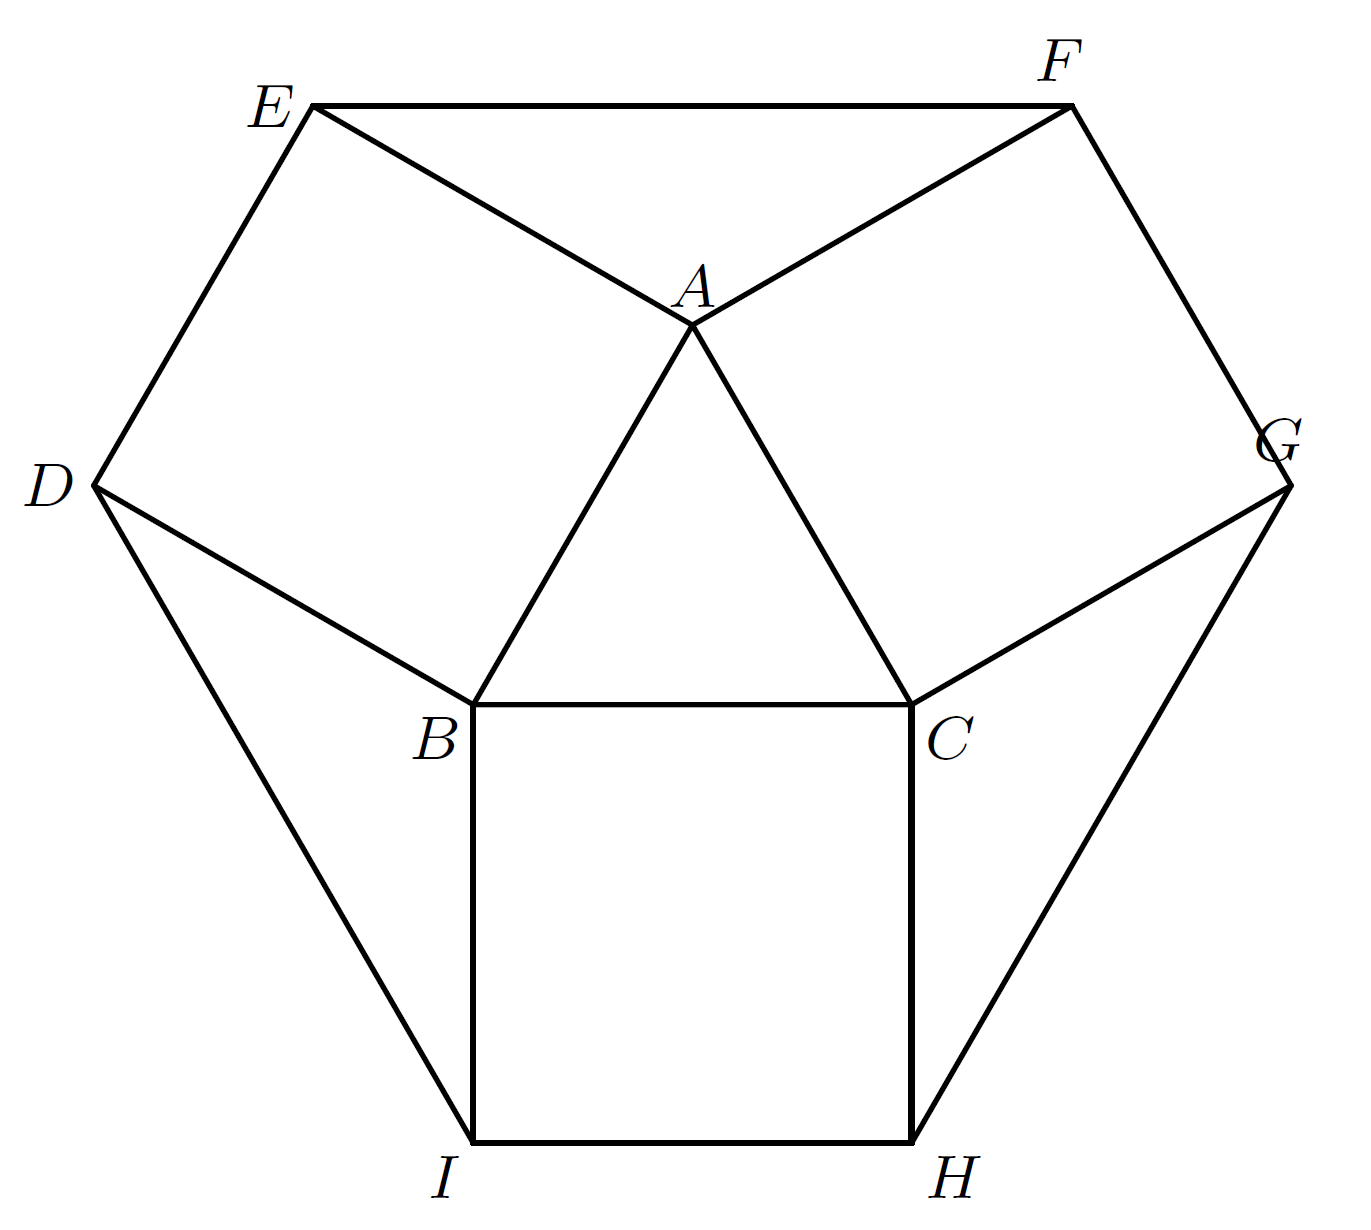
\includegraphics[height=2in]{hex}
\end{center}
$\textbf{(A)}\ \dfrac{12+3\sqrt3}4\qquad\textbf{(B)}\ \dfrac92\qquad\textbf{(C)}\ 3+\sqrt3\qquad\textbf{(D)}\ \dfrac{6+3\sqrt3}2\qquad\textbf{(E)}\ 6$
\end{problem}

\begin{problem}
Rhombus $ABCD$ is similar to rhombus $BFDE$. The area of rhombus $ABCD$ is 24, and $\angle BAD = 60^\circ$. What is the area of rhombus $BFDE$?
 \begin{center}
    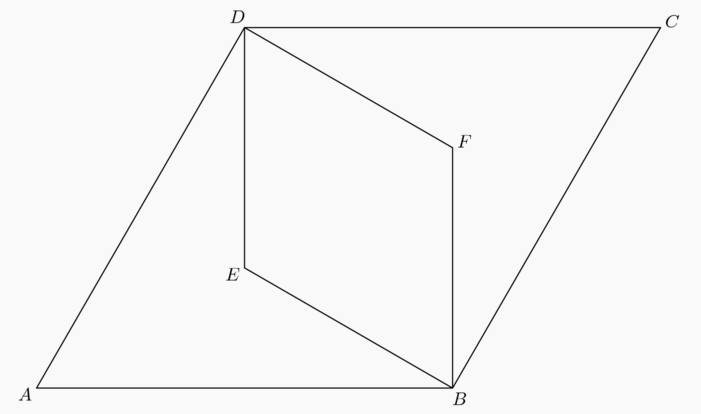
\includegraphics[width = 3in]{rhombus}
    \end{center}
$\textrm{(A) } 6 \qquad \textrm{(B) } 4\sqrt {3} \qquad \textrm{(C) } 8 \qquad \textrm{(D) } 9 \qquad \textrm{(E) } 6\sqrt {3}$
\end{problem}

\begin{problem}
Three congruent isosceles triangles are constructed with their bases on the sides of an equilateral triangle of side length $1$. The sum of the areas of the three isosceles triangles is the same as the area of the equilateral triangle. What is the length of one of the two congruent sides of one of the isosceles triangles? \vspace{0.2in}

$\textbf{(A) }\dfrac{\sqrt3}4\qquad \textbf{(B) }\dfrac{\sqrt3}3\qquad \textbf{(C) }\dfrac23\qquad \textbf{(D) }\dfrac{\sqrt2}2\qquad \textbf{(E) }\dfrac{\sqrt3}2$
\end{problem}

\begin{problem}
In triangle $ABC$, $AB = 13$, $BC = 14$, $AC = 15$. Let $D$ denote the midpoint of $\overline{BC}$ and let $E$ denote the intersection of $\overline{BC}$ with the bisector of angle $BAC$. Which of the following is closest to the area of the triangle $ADE$? \vspace{0.2in}

$\text {(A)}\ 2 \qquad \text {(B)}\ 2.5 \qquad \text {(C)}\ 3 \qquad \text {(D)}\ 3.5 \qquad \text {(E)}\ 4$
\end{problem}

\begin{problem}
A right triangle has perimeter $32$ and area $20$. What is the length of its hypotenuse? \vspace{0.2in}

$\mathrm{(A)}\ \frac{57}{4}\qquad\mathrm{(B)}\ \frac{59}{4}\qquad\mathrm{(C)}\ \frac{61}{4}\qquad\mathrm{(D)}\ \frac{63}{4}\qquad\mathrm{(E)}\ \frac{65}{4}$
\end{problem}

\begin{problem}
A circle centered at $O$ has radius $1$ and contains the point $A$. The segment $AB$ is tangent to the circle at $A$ and $\angle AOB = \theta$. If point $C$ lies on $\overline{OA}$ and $\overline{BC}$ bisects $\angle ABO$, then $OC =$
\begin{center}
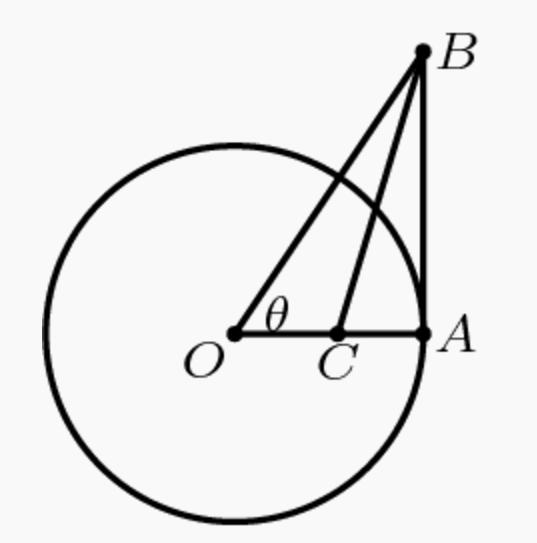
\includegraphics[width=2in]{circle}
\end{center}
$\text {(A)}\ \sec^2 \theta - \tan \theta \qquad \text {(B)}\ \frac 12 \qquad \text {(C)}\ \frac{\cos^2 \theta}{1 + \sin \theta}\qquad \text {(D)}\ \frac{1}{1+\sin\theta} \qquad \text {(E)}\ \frac{\sin \theta}{\cos^2 \theta}$
\end{problem}
\newpage
\section{Circles}
\subsection{Introduction}
Recall a question we had on the worksheet last week:
\begin{center}
\textit{``Draw the locus of points that are exactly 3 cm away from a point A''}
\end{center}

Maybe you tried it...maybe you didn't. But hopefully now that you've done it, you realize that I was asking you to draw a circle all along! So what is so mystical about the circle? The ancients seemed to fawn over its perfection and worship its impeccable symmetry. What we will find out is that there are many interesting geometric properties about circles.

\subsection{Basics}
\begin{center}
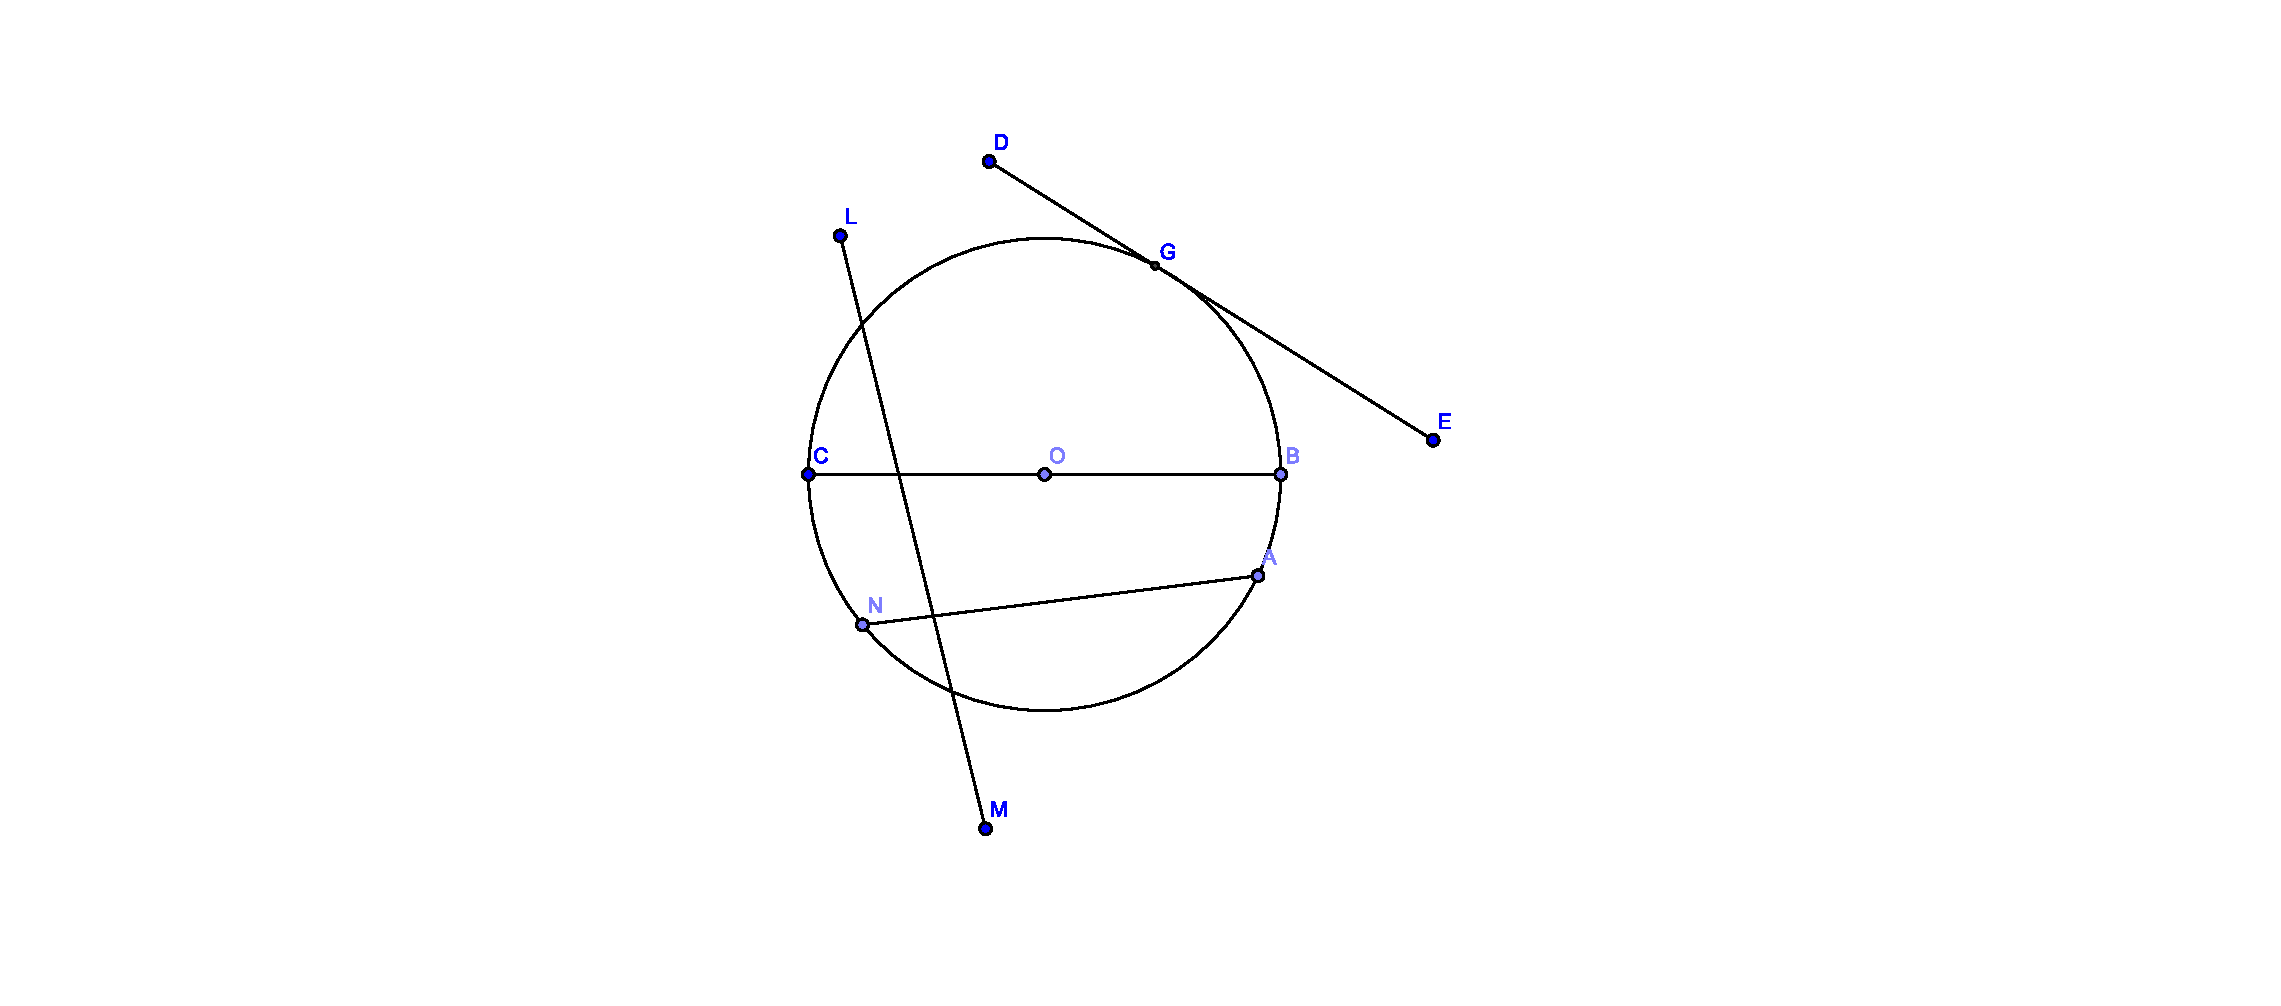
\includegraphics[height=3in, trim={2cm 1cm 0 1.1cm}]{circle1}
\end{center}
We start off with a circle, which as we see from our definition earlier, is a collection of points that are equidistant from a particular point. In general, we often use \textbf{O} as the center of the circle (origin). Now, on this circle we can draw many special lines:
\begin{itemize}
    \item The \textbf{radius} is the line from the center to any point on the circle On the diagram, $\overline{OC}$ and $\overline{OB}$ are both radii. 
    \item The \textbf{diameter} is defined to be the line through the center of the circle. Note that the length of the diameter is $2r$, where $r$ is the radius of the circle.
    \item A \textbf{chord} is any line connecting any two non-equal points on the circle. Note that the diameter is a special case of a chord
    \item A \textbf{secant} is any line intersecting the circle at two points
    \item A \textbf{tangent} is any line intersecting the circle at exactly one point
\end{itemize}

\subsubsection{$\pi$}
In order to prove some basic theorems, we have to begin with this theorem,

\begin{theorem}
The ratio of the circumference of a circle to its diameter is $\pi$
\end{theorem}

Or in equation form, $\text{Circumference} = \pi d = 2\pi r$. As you guys probably already know, $\pi = 3.14159\cdots$. With this knowledge, we can prove the area of a circle.

\begin{theorem}
The area of a circle is $\pi r^2$
\end{theorem}

\subsection{Angles}
Now that we know what a circle is, it is natural to begin a discussion of how angles are related to a circle. 
\begin{center}
\begin{tikzpicture}
% the origin
\coordinate (O) at (0,0);
% the circle and the dot at the origin
\draw (O) node[circle,inner sep=1.5pt,fill] {} circle [radius=3cm];
\draw (O) node[left] {$O$};
\draw (3cm,0) node[right] {$A$};
\draw (60:3cm) node[right, above] {$B$};
% the ``\theta'' arc
\draw 
  (3cm,0) coordinate (xcoord) -- 
  node[midway,below] {$r$} (O) -- 
  (60:3cm) coordinate (slcoord)
  pic [draw,->,angle radius=1cm,"$\theta$"] {angle = xcoord--O--slcoord};

\end{tikzpicture}
\end{center}

We define an \textbf{angle} to be the figure formed by two \textbf{rays}. If we consider the diagram above, the angle has \textbf{measure} $\theta$ and \textbf{subtends} $\arc{AB}$. We usually refer to an angle to either the vertex it is at, or to avoid confusion, the acute angle formed by three points---in our case, $\angle ABO$ or $\angle BOA$.

As you may know, a circle contains $360\degree$. It turns out, this number was entirely arbitrary, as in we could've chosen 100 or 1000. But we have 360, because it's divisible by a bunch of numbers, and that's what we still use today. There is also another way to define angles, called \textbf{radians}. The conversion for this is 
$$1 = \frac{360\degree}{2\pi}.$$
Until you are in higher math or physics, you won't be needing radians too much.

When we have an angle, we can classify it into three categories, 
\begin{itemize}
    \item \textbf{Acute}: $<90\degree$
    \item \textbf{Right, Perpendicular, Orthogonal}: $=90\degree$
    \item \textbf{Obtuse}: $>90\degree$
    \item \textbf{Reflex}: $>180\degree$
\end{itemize}
We also say two angles whose sum is $90\degree$ are \textbf{complementary}, and two angles whose sum is $180\degree$ is \textbf{supplementary}. If you ever get confused, just remember that ``a compliment is the \textit{right} thing to do!'' Note that this compliment is spelled differently, but nonetheless still is useful for memorizing the term. 
\newpage
\subsubsection{Lines in a Circle}
From our diagram above, it is clear that the angle formed by the rays equals the arc of the circle. This type of angle is known as a \textbf{central angle}, and is the easiest to deal with. For the other angles, they have certain formulas. We will look at them and try to prove their properties as well. \vspace{0.2in}

\begin{minipage}{0.6\textwidth}
\subsubsection{Inscribed Angle}
\begin{center}
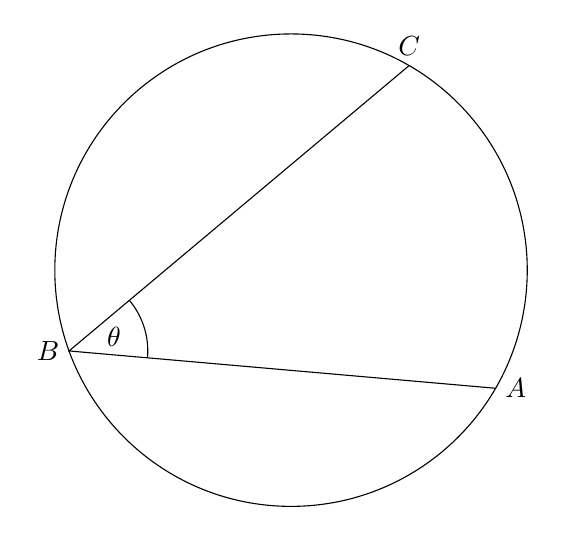
\begin{tikzpicture}
\draw (0,0) circle  [radius = 3cm];
\draw (-30:3cm) coordinate (a) node[right] {$A$}  --
 (200:3cm) coordinate (b) node[left] {$B$}  --
(60:3cm) coordinate (c) node[right, above] {$C$} ;
\pic [draw,-,angle radius=1cm,"$\theta$"] {angle = a--b--c};
\end{tikzpicture}
\end{center}
\end{minipage}
\begin{minipage}{0.35\textwidth}
$$\theta = \frac{\arc{AC}}{2}.$$
\end{minipage}

\vspace{1in}

\subsubsection{Two Secants}
\begin{minipage}{0.6\textwidth}
\begin{center}
\begin{tikzpicture}
\draw (0,0) circle  [radius = 3cm];
\draw (15:3cm) node[right] {$\alpha$};
\draw (190:3cm) node[right] {$\beta$};
\draw (-30:3cm) coordinate (a) node[right] {$A$}  --
 (-5cm, -1cm) coordinate (b) node[left] {$B$}  --
(60:3cm) coordinate (c) node[right, above] {$C$} ;
\pic [draw,-,angle radius=1cm,"$\theta$"] {angle = a--b--c};
\end{tikzpicture}
\end{center}
\end{minipage}
\begin{minipage}{0.35\textwidth}
$$\theta = \frac{\alpha-\beta}{2} $$
Note that there is a similar formula for two tangents.
\end{minipage}

\subsubsection{Tangent and Chord}
\begin{minipage}{0.6\textwidth}
\begin{center}
\begin{tikzpicture}
\draw (0,0) circle  [radius = 3cm];
\draw (3,-3) coordinate (a) node[right] {$A$}--
(-3,-3) coordinate (b) node[left] {$B$};
\draw (0,-3) coordinate (o) node[below] {$D$}--
(60:3cm) coordinate (c) node[right, above] {$C$} ;
\pic [draw,-,angle radius=1cm,"$\theta$"] {angle = a--o--c};
\end{tikzpicture}
\end{center}
\end{minipage}
\begin{minipage}{0.35\textwidth}
This is actually just a special case of the theorem above.
$$\theta = \frac{\arc{DC}}{2}$$
\end{minipage}

\vspace{1in}

\subsubsection{Two Chords}
\begin{minipage}{0.6\textwidth}
\begin{center}
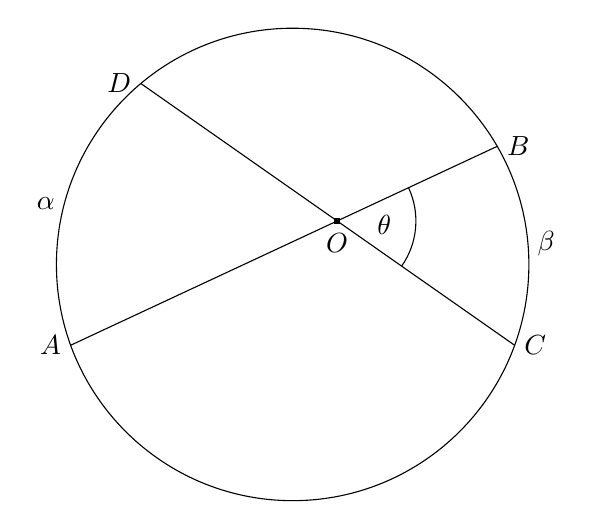
\begin{tikzpicture}
\draw (0,0) circle  [radius = 3cm];
\draw (165:3cm) node[left] {$\alpha$};
\draw (5:3cm) node[right] {$\beta$};
\draw[name path = a--b] (200:3cm) coordinate (a) node[left] {$A$}  --
 (30:3cm) coordinate (b) node[right] {$B$};
 \draw[name path = c--d] (-20:3cm) coordinate (c) node[right] {$C$}  --
 (130:3cm) coordinate (d) node[left] {$D$};
\path [name intersections={of=a--b and c--d,by=o}];
\node [fill=black,inner sep=1pt,label=-90:$O$] at (o) {};
\pic [draw,-,angle radius=1cm,"$\theta$"] {angle = c--o--b};
\end{tikzpicture}
\end{center}
\end{minipage}
\begin{minipage}{0.35\textwidth}
$$\theta = \frac{\alpha+\beta}{2}$$
\end{minipage}

\subsection{Problems}
\begin{problem}
Prove that the angle formed by the intersection of a tangent and a radius of a circle is $90\degree$.
\end{problem}
\begin{problem}
Show that any triangle inscribed in a circle with the diameter as one of its sides must be a right triangle.
\end{problem}
\begin{problem}
Show that the length of the segment connecting the $90\degree$ vertex of a right triangle to the midpoint of the hypotenuse is equal to half the hypotenuse.
\end{problem}
\begin{problem}
Prove that the angles of a triangle must sum to $180\degree$.
\end{problem}

\clearpage
\begin{problem}
(MATHCOUNTS State Sprint \#30 2009) In the figure, the measure of angle RAS is 74 degrees, and the measure of angle RTB is 28 degrees. What is the measure of minor arc BR, in degrees?
\begin{center}
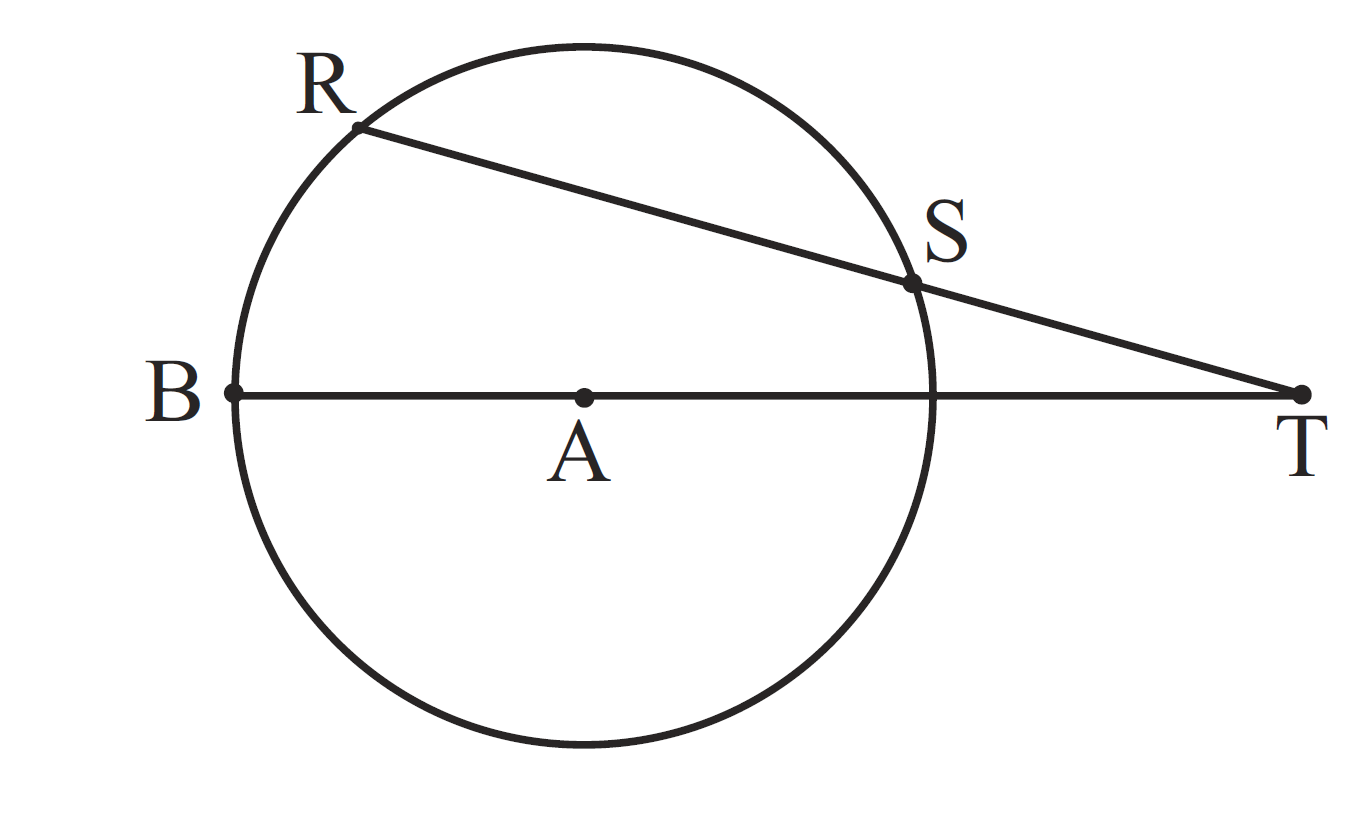
\includegraphics[height=2in]{circleMath}
\end{center}
\end{problem}
\vspace{1.5in}
\section{Power of a Point}
As you can imagine, these theorems are very powerful. But in all seriousness, now that we've done angles, it's time to learn about how side lengths are related in circles.

\subsubsection{Equal Tangents}
\begin{minipage}{0.6\textwidth}
\begin{center}
\begin{tikzpicture}
\draw (0,0) circle  [radius = 3cm];
\draw (111:3cm) coordinate (a) node[above] {$B$}  --
 (-6cm, 0.3cm) coordinate (b) node[left] {$A$}  --
(235:3cm) coordinate (c) node[below ] {$C$} ;
\end{tikzpicture}
\end{center}
\end{minipage}
\begin{minipage}{0.35\textwidth}
\begin{theorem}
Two tangents from the same point to a circle are always equal.
\end{theorem}
In other words, $AB = AC$.
\end{minipage}

\subsubsection{General Case}
\begin{minipage}{0.6\textwidth}
\begin{center}
\begin{tikzpicture}
\draw (0,0) circle  [radius = 3cm];
\draw (141:3cm) node[left] {$B$};
\draw (-162:3cm) node[left] {$D$};
\draw (80:3cm) coordinate (a) node[above] {$C$}  --
 (-6cm, 0.3cm) coordinate (b) node[left] {$A$}  --
(-50:3cm) coordinate (c) node[below ] {$E$} ;
\end{tikzpicture}
\end{center}
\end{minipage}
\begin{minipage}{0.35\textwidth}
$$(\overline{AB})(\overline{AC})=(\overline{AD})(\overline{AE})$$
\end{minipage}

\subsubsection{Special Case}
\begin{minipage}{0.6\textwidth}
\begin{center}
\begin{tikzpicture}
\draw (0,0) circle  [radius = 3cm];
\draw (205:3cm) node[left] {$C$};
\draw (111:3cm) coordinate (a) node[above] {$B$}  --
 (-6cm, 0.3cm) coordinate (b) node[left] {$A$}  --
(-70:3cm) coordinate (c) node[below ] {$D$} ;
\end{tikzpicture}
\end{center}
\end{minipage}
\begin{minipage}{0.35\textwidth}
A special case of the theorem above.
$$(\overline{AC})(\overline{AD}) = \overline{AB}^2$$
\end{minipage}

\subsubsection{Two Chords}
\begin{minipage}{0.6\textwidth}
\begin{center}
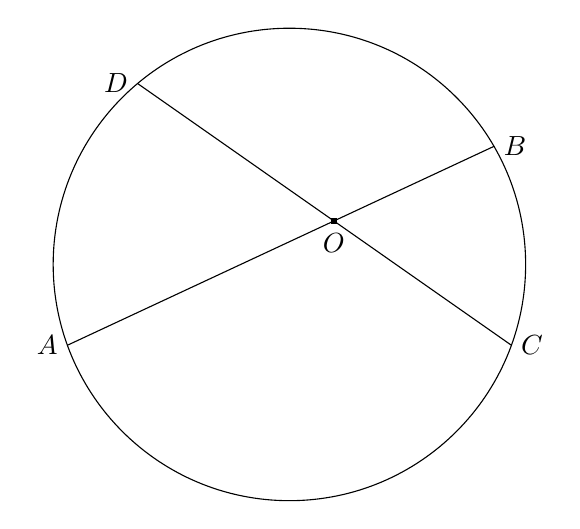
\begin{tikzpicture}
\draw (0,0) circle  [radius = 3cm];
\draw[name path = a--b] (200:3cm) coordinate (a) node[left] {$A$}  --
 (30:3cm) coordinate (b) node[right] {$B$};
 \draw[name path = c--d] (-20:3cm) coordinate (c) node[right] {$C$}  --
 (130:3cm) coordinate (d) node[left] {$D$};
\path [name intersections={of=a--b and c--d,by=o}];
\node [fill=black,inner sep=1pt,label=-90:$O$] at (o) {};
\end{tikzpicture}
\end{center}
\end{minipage}
\begin{minipage}{0.35\textwidth}
$$(\overline{OA})(\overline{OB})=(\overline{OD})(\overline{OC})$$
\end{minipage}

\subsection{Problems}
\begin{problem}
Prove that if a circle can be inscribed in quadrilateral $ABCD$, then $AB+CD=BC+AD$.
\end{problem}
\begin{problem}
Express all the line segments of a triangle purely in terms of its side lengths when its incircle is drawn.
\end{problem}
\begin{problem}
Prove that if a radius bisects a chord, then it is perpendicular to the chord.
\end{problem}
\begin{problem}
Prove that if a radius intersects a chord perpendicularly, then it must bisect the chord.
\end{problem}
\begin{problem}
(AHSME 1954) A point $P$ is outside a circle and is $13$ inches from the center. A secant from $P$ cuts the circle at $Q$ and $R$ so that the external segment of the secant $PQ$ is $9$ inches and $QR$ is $7$ inches. The radius of the circle is:

$\textbf{(A)}\ 3" \qquad \textbf{(B)}\ 4" \qquad \textbf{(C)}\ 5" \qquad \textbf{(D)}\ 6"\qquad\textbf{(E)}\ 7"$
\end{problem}
\begin{problem}
(AHSME 1956) The points $A$, $B$, and $C$ are on circle $O$. THe tangent line at $A$ and the secant $BC$ intersect at $P$, $B$, lying between $C$ and $P$. If $BC=20$ and $PA=10\sqrt{3}$, find $PB$.
\end{problem}
\begin{problem}
The figure below, $O$ is the center of circle $O$, $\overline{AD}=6$, $\overline{OD}=9$, and $\overline{AB} = 2\overline{BC}$. Find $\overline{AB}$.
\begin{center}
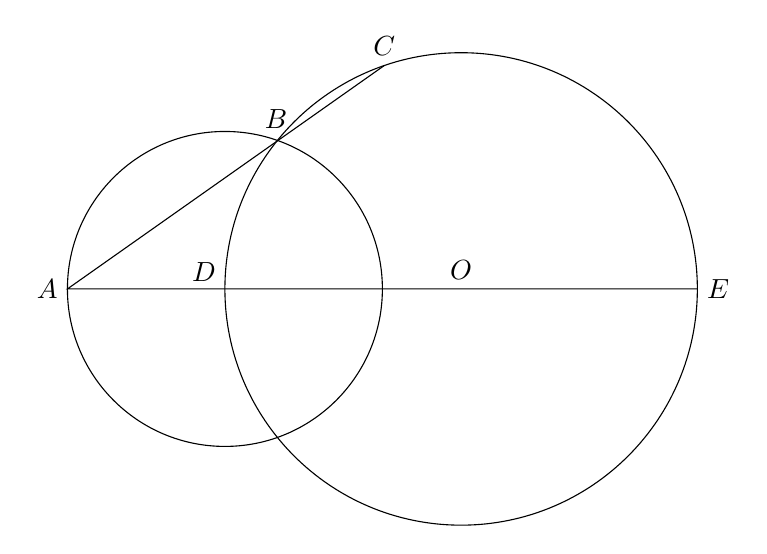
\begin{tikzpicture}
\draw (0,0) circle  [radius = 3cm];
\draw (0,0) node[above] {$O$};
\draw (-3,0) circle [radius = 2.0cm]; 
\draw (134:3cm) node[left] {$B$};
\draw (176:3cm) node[left] {$D$};
\draw (109:3cm) coordinate (a) node[above] {$C$}  --
 (-5.0cm, 0) coordinate (b) node[left] {$A$}  --
(0:3cm) coordinate (c) node[right] {$E$} ;
\end{tikzpicture}
\end{center}
\end{problem}
\begin{problem}
Two tangents from an external point $P$ are drawn to a circle and intersect it at $A$ and $B$. A third tangent meets the circle at $T$, and the tangents $\overline{PA}$ and $\overline{PB}$ at points $Q$ and $R$, respectively. If $AB=20$, then find the perimeter of $\triangle PQR$.
\end{problem}
\newpage 
\section{Areas}
The purpose of this lecture is to introduce some area problem solving techniques that extend beyond the basic formulas for fundamental shapes.
	
	\subsection{Traditional Equations}
	\textbf{Heron's Formula} \textit{The area of a triangle whose sides have lengths $a$, $b$, and $c$ is
  $$ A = \sqrt{s(s-a)(s-b)(s-c)}$$}	
	
	\begin{problem}
	Find the area of a triangle with side lengths 5, 7, 8.
	\end{problem}
	
	\begin{problem}
	Find the area of a triangle with side lengths 13, 14, 15.
	\end{problem}
	
	\noindent \textbf{Brahmagupta's Theorem} \textit{The area $K$ of a cyclic quadrilateral whose sides have lengths $a$, $b$, $c$, $d$ as
  $$ K=\sqrt{(s-a)(s-b)(s-c)(s-d)}$$}

	\begin{problem}
	Find the area of quadrilateral $ABCD$ if it is inscribed in the circle below.
	\begin{center}
	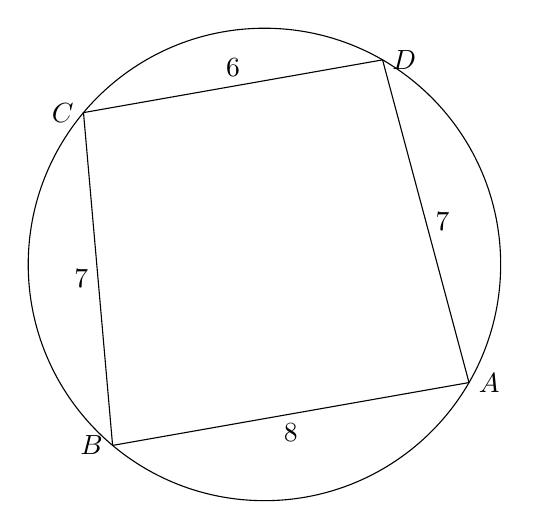
\begin{tikzpicture}
		\draw (0,0) circle  [radius = 3cm];
		\draw (230:3cm) node[left] {$B$};
		\draw (140:3cm) node[left] {$C$};
		\draw (60:3cm) node[above, right] {$D$};
		\draw (-30:3cm) coordinate (a) node[right] {$A$}  --
		 (230:3cm) coordinate (b) node[midway, below] {$8$}  --
		(140:3cm) coordinate (c) node[midway, left] {$7$} --
		(60:3cm) coordinate (d) node[midway, above] {$6$}-- (-30:3cm) coordinate (e) node[midway, right] {$7$};
	\end{tikzpicture}
	\end{center}
	\end{problem}
	
	\clearpage

	\subsection{Pick's Theorem}
	\begin{theorem}
	Given a simple polygon constructed on a unit grid such that all the polygon's vertices are lattice points, the area of this polygon is 
    $$A = i + \frac{b}{2} - 1, $$
		where $i$ is the number of lattice points in the interior located in the polygon and the $b$ is the number of lattice points on the boundary of the polygon.
	\end{theorem}
	%know how to do the proof
	
	\begin{problem}
	What is the area of the polygon in the diagram below? (this is a unit square grid)
	\begin{center}
	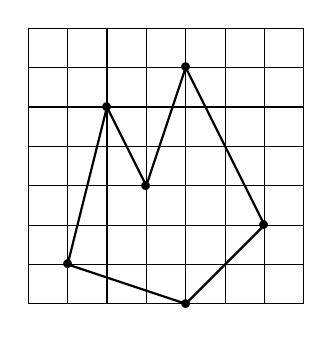
\begin{tikzpicture}[scale=0.5]
			\draw (0,0) grid (7,7);
			\draw (1,1) node[scale=3]{.};
			\draw [thick] (1,1)--(2,5);
			\draw (2, 5) node[scale=3]{.};
			\draw [thick] (2, 5)--(3, 3);
			\draw (3,3) node[scale=3]{.};
			\draw [thick] (3,3)--(4, 6);
			\draw (4, 6) node[scale=3]{.};
			\draw [thick] (4, 6)--(6, 2);
			\draw (6, 2) node[scale=3]{.};
			\draw [thick] (6,2)--(4,0);
			\draw (4,0) node[scale=3]{.};
			\draw [thick] (4,0)--(1,1);
	\end{tikzpicture}
	\end{center}
	\end{problem}
	
	\begin{problem}
	What is the area of the polygon in the diagram below? (this is a unit square grid)
	\begin{center}
	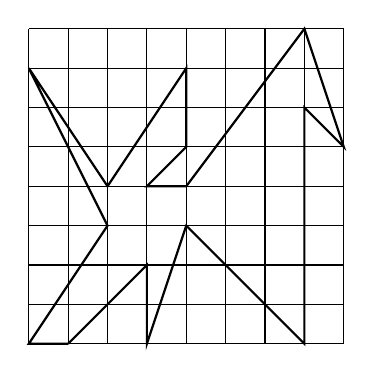
\begin{tikzpicture}[scale=0.5]
		\draw (0,0) grid (8,8);
		\draw [thick] (1,0)--(3,2)--(3,0)--(4,3)--(7,0)--(7,6)--(8,5)--(7,8)--(4,4)--(3,4)--(4,5)--(4,7)--(2,4)--(0,7)--(2,3)--(0,0)--(1,0);
	\end{tikzpicture}
	\end{center}
	\end{problem}

	\subsection{Shoelace Theorem}
	\begin{theorem}
	Suppose the polygon $P$ has vertices $(a_1, b_1)$, $(a_2, b_2)$, ... , $(a_n, b_n)$, listed in clockwise order. Then the area of $P$ is
	\[\dfrac{1}{2} |(a_1b_2 + a_2b_3 + \cdots + a_nb_1) - (b_1a_2 + b_2a_3 + \cdots + b_na_1)|\] 
	\end{theorem}
	
	In case you're wondering where the shoelace formula gets its name, it's because when you list out the coordinates in a matrix,
	 $$\begin{bmatrix} a_1 & b_1 \\ a_2 & b_2\\ \vdots & \vdots \\ a_n & b_n \end{bmatrix},$$
	you'll find out that the multiplication is in a shoelace cross pattern.
	
	\clearpage
	\begin{problem}
	Find the area of the following polygon.
	\begin{center}
	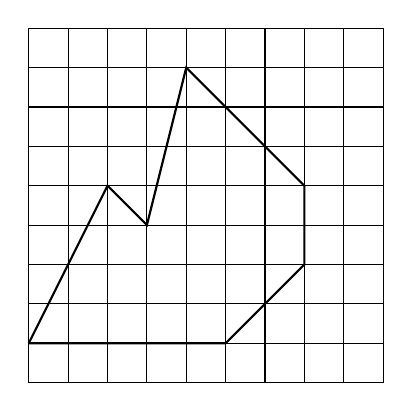
\begin{tikzpicture}[scale=0.5]
	\draw (0,0) grid (9,9);
	\draw [thick] (0,1)--(2, 5)--(3,4)--(4,8)--(6,6)--(7,5)--(7,3)--(6,2)--(5,1)--(3,1)--(0,1);
	\end{tikzpicture}
	\end{center}
	\end{problem}
	
	\begin{problem}
	Find the area of the following polygon with the given coordinates: $(1.2,1), (2.4, 0.5), (8,3.2), \\ (7,6.5), (6,7.2), (3,7.6), (1.2,1) $
	\begin{center}
	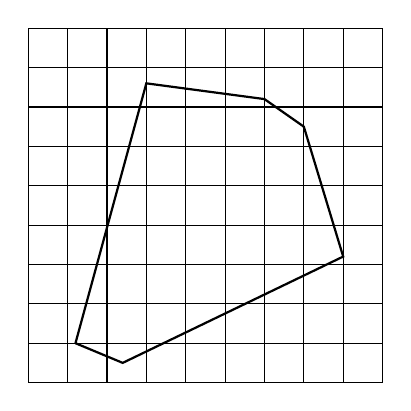
\begin{tikzpicture}[scale=0.5]
	\draw (0,0) grid (9,9);
	\draw [thick] (1.2,1)--(2.4, 0.5)--(8,3.2)--(7,6.5)--(6,7.2)--(3,7.6)--(1.2,1);
	
	\end{tikzpicture}
	\end{center}
	\end{problem}
	
	\subsection{Problems}
	\begin{problem}
	An equiangular octagon has four sides of length 1 and four sides of length $\frac{\sqrt{2}}{2}$, arranged so that no two consecutive sides have the same length. What is the area of the octagon?

$\mathrm{(A) \ } \frac72\qquad \mathrm{(B) \ } \frac{7\sqrt2}{2}\qquad \mathrm{(C) \ } \frac{5+4\sqrt2}{2}\qquad \mathrm{(D) \ } \frac{4+5\sqrt2}{2}\qquad \mathrm{(E) \ } 7$ 
	\end{problem}
	
	\begin{problem}
	Points $E$ and $F$ are located on square $ABCD$ so that $\triangle BEF$ is equilateral. What is the ratio of the area of $\triangle DEF$ to that of $\triangle ABE$? 
	
	\begin{center}
	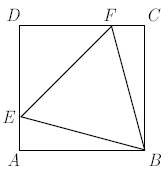
\includegraphics[width=1.6in]{squareTri}
	\end{center}
	\end{problem}
	
	\begin{problem}
	A circle is inscribed in a square, then a square is inscribed in this circle, and finally, a circle is inscribed in this square. What is the ratio of the area of the smaller circle to the area of the larger square?

$\mathrm{(A)} \frac{\pi}{16} \qquad \mathrm{(B)} \frac{\pi}{8} \qquad \mathrm{(C)} \frac{3\pi}{16} \qquad \mathrm{(D)} \frac{\pi}{4} \qquad \mathrm{(E)} \frac{\pi}{2}$
	\end{problem}
	
	\clearpage
	\begin{problem}
	Given that the area of $\triangle ABC$ is 196, and $DB = 6AD$, find the area of $\triangle CDB$.
	\begin{center}
	\begin{tikzpicture}
		\draw (0,0) node [below] {$A$};
		\draw (7,0) node [below]{$B$};
		\draw (5,3) node [above]{$C$}; 
		\draw (1,0) node [below]{$D$};
		\draw (0,0)--(7,0)--(5,3)--(0,0);
		\draw (5,3)--(1,0);
	\end{tikzpicture}
	\end{center}
	\end{problem}
	
	\vspace{0.5in}
	
	\begin{problem}
	Given that $AB=$ and $BC=$, find the area of the shaded region.
	\begin{center}
		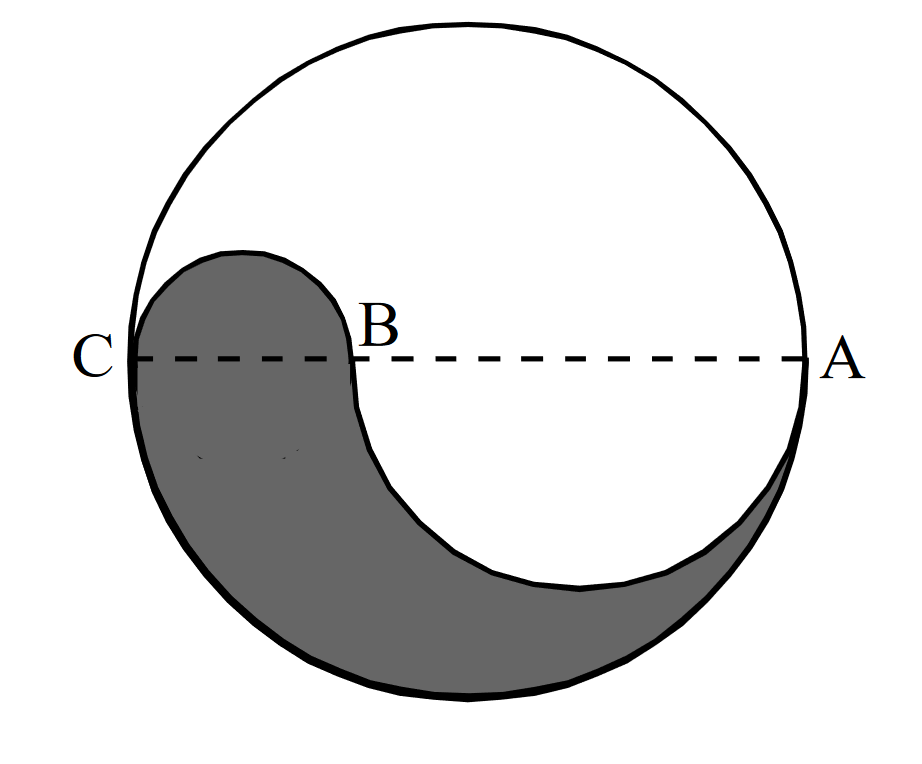
\includegraphics[width=2in]{circle11}
	\end{center}
	\end{problem}
	
	\vspace{0.6in}
	
	\begin{problem}
	Find the area of the shaded region.
	\begin{center}
		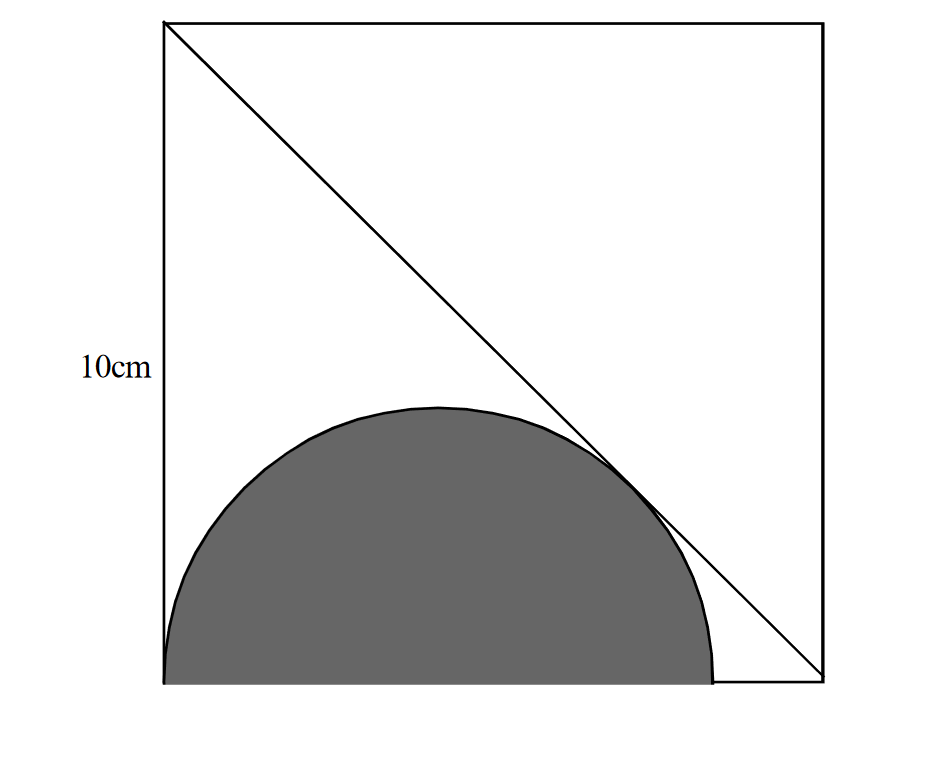
\includegraphics[width=3in]{circle2}
	\end{center}
	\end{problem}
	
	\clearpage
	\begin{problem}
	Find the area of the shaded region.
	\begin{center}
		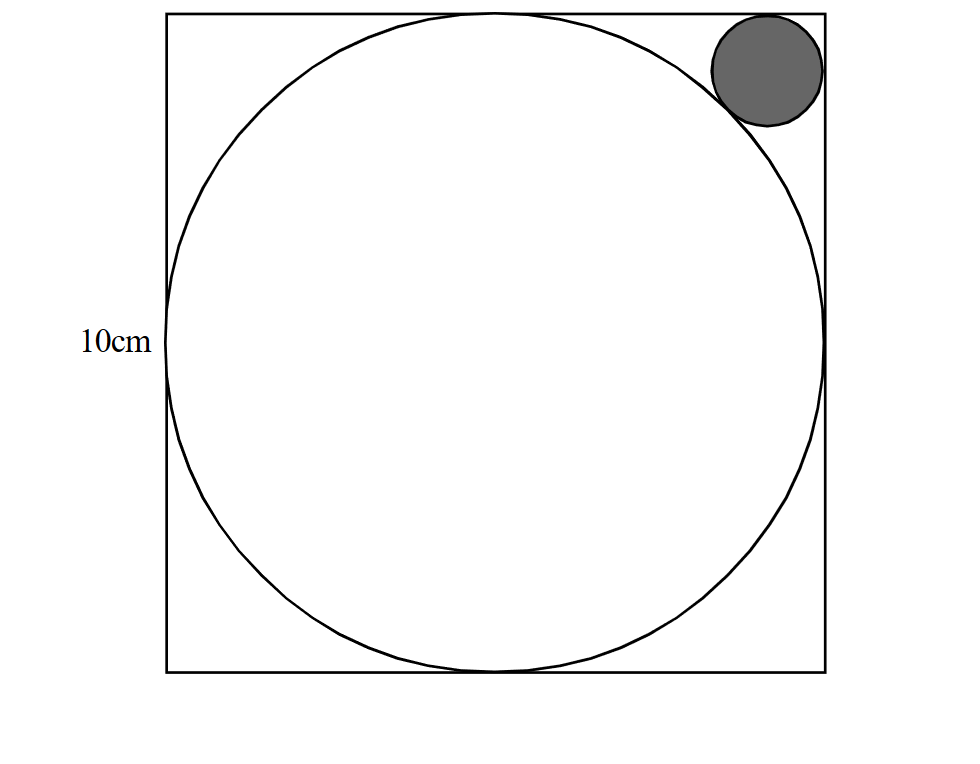
\includegraphics[width=3in]{circle3}
	\end{center}
	\end{problem}
	
	\vspace{1.5in}
	
	\begin{problem}
	Find the area of the shaded region.
	\begin{center}
		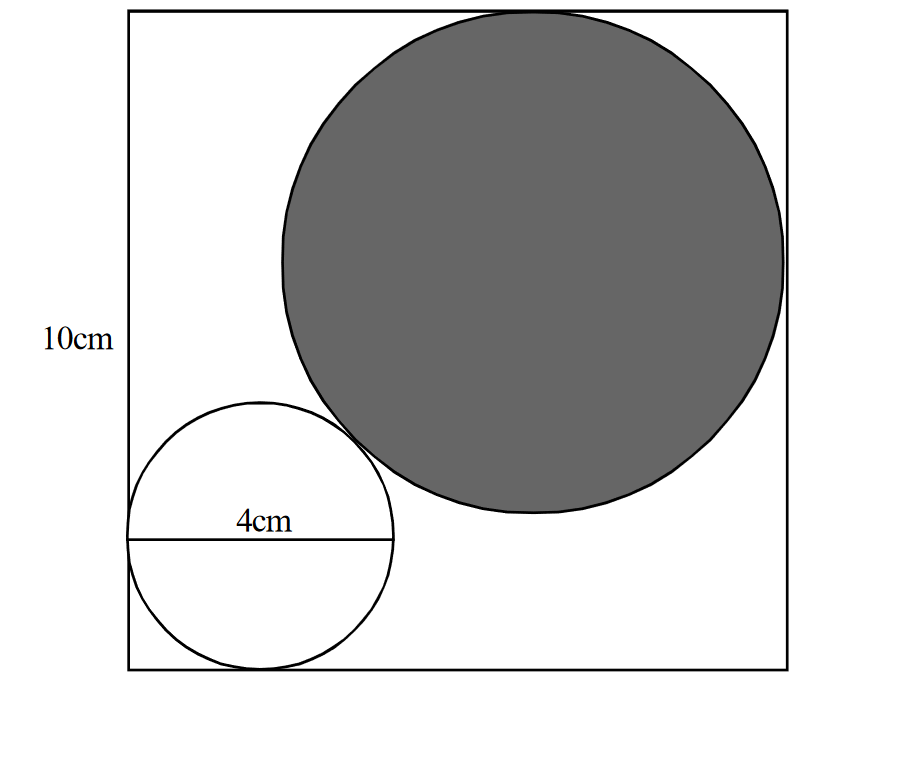
\includegraphics[width=3in]{circle4}
	\end{center}
	\end{problem}
	
	\clearpage
	\begin{problem}
	Find the area of the shaded region.
	\begin{center}
		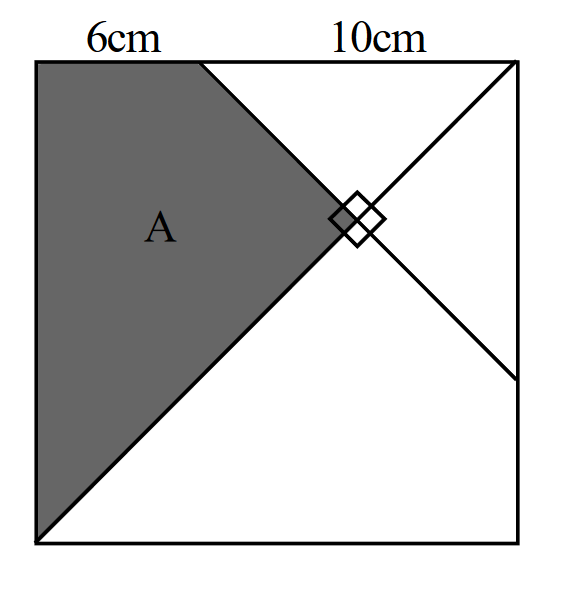
\includegraphics[width=3in]{square}
	\end{center}
	\end{problem}
	
	\vspace{1in}
	
	\begin{problem}
	Find the area of the shaded region.
	\begin{center}
		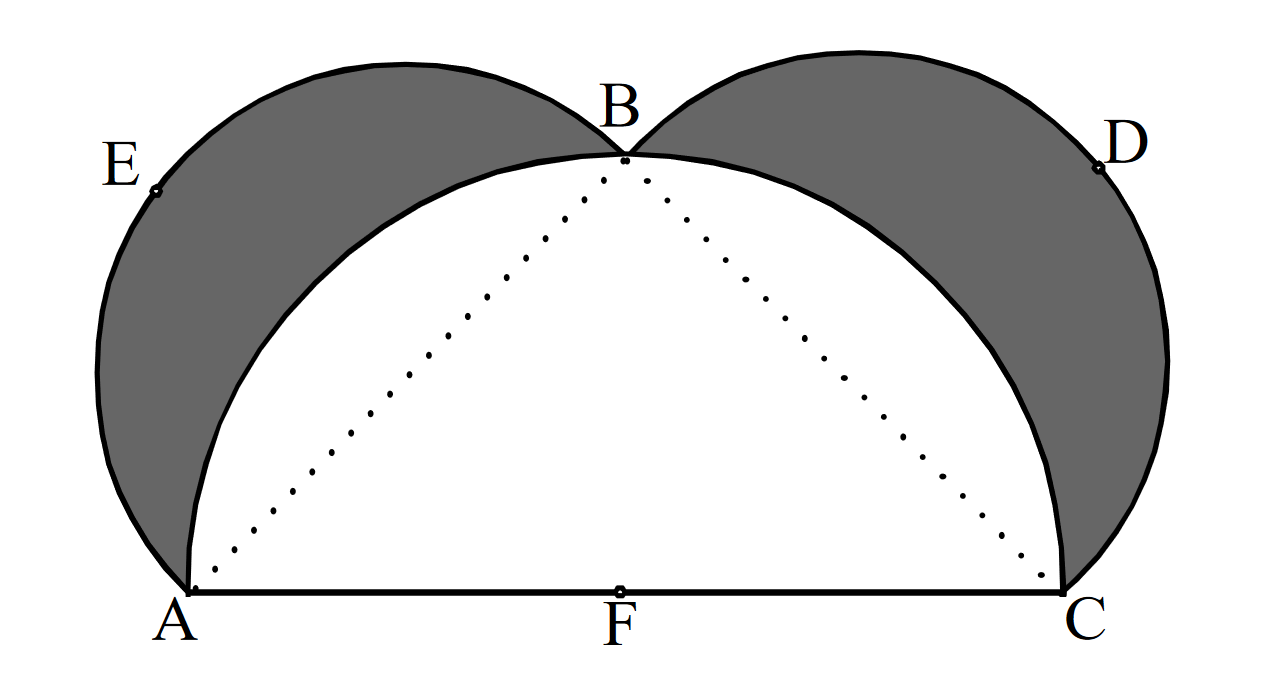
\includegraphics[width=3.5in]{mickeyMouse}
	\end{center}
	\end{problem}
\newpage 
\section{Mass Points}
The purpose of this lesson is to provide an introduction to mass points---a technique commonly used to find triangle length proportions. The advantage of using mass points is that it can simplify very complex problems using the concepts of simple physics.

\subsection{Introduction}
    \begin{definition}
    A \textbf{mass point} consists of a mass $m$ and a point $P$, which is denoted as $(m,P)$, or sometimes $mP$.
    \end{definition}
    \begin{definition}
    Two mass points $(m_1,P_1), (m_2, P_2)$ \textbf{coincide}, or are equivalent, \textit{iff} $m_1=m_2$ and $P_1=P_2$.
    \end{definition}
    \begin{definition} The sum of two mass points $mP$ and $nQ$ has mass $m + n$ and point $R$ where $R$ is the point on $PQ$ such that $PR:RQ = n:m$. In other words, $R$ is the fulcrum point that perfectly balances the points $P$ and $Q$.
    \end{definition}
	\begin{definition}
	If one mass point is multiplied by a scalar $k$, then all other mass points in the system must be multiplied by $k$ as well for the mass relations to hold.
    \end{definition}
	
	\subsubsection{Physics Examples}
	The classic lever problem involves balancing masses on opposite ends of a seesaw. I won't go into the complicated physics of this problem, but the result is that in order for the seesaw to be balanced, 
	$$m_1 d_1 = m_2 d_2.$$
\begin{problem}
    Bob and Jane are sitting on opposite ends of a balanced seesaw. If Bob weighs 150 lb and Jane weighs 100 lb, what is the ratio of Bob's to Jane's distance from the fulcrum? (assume the seesaw itself has negligible mass)
\end{problem}
\begin{problem}
    An elephant and I are standing 10 ft away from the fulcrum of a very long seesaw. If the elephant is 8,000 lbs and I am 160 lbs, how many feet back do I have to walk in order to balance the elephant?
\end{problem}
    
\subsection{Mass Point Problems}
\subsubsection{Easy Cevians}
\begin{problem}
In $\triangle ABC$, side $BC$ is divided by $D$ in a ratio of 5 to 2 and $BA$ is divided by $E$ in a ratio of 3 to 4. Find the ratios in which $F$ divides the cevians $AD$ and $CE$, i.e. find $EF : FC$ and $DF : FA$.
\begin{center}
	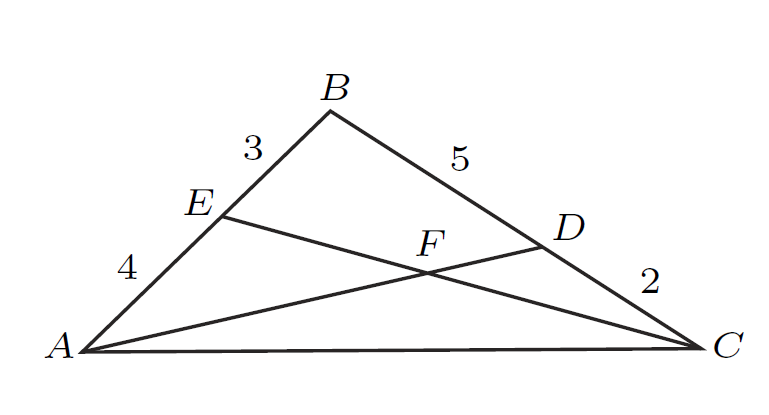
\includegraphics[width=2.5in]{cevian}
	\end{center}
\end{problem}
\begin{problem}
Point $E$ is selected on side $AB$ of $\triangle ABC$ in such a way that $AE : EB = 1 : 3$ and point $D$ is selected on side $BC$ so that $CD : DB = 1 : 2$. The point of intersection of $AD$ and $CE$ is $F$. Find $\frac{EF}{FC}+\frac{AF}{FC}$.
\end{problem}
\begin{problem}
In $\triangle ABC$ points $D$ and $E$ lie on $BC$ and $AC$, respectively. If $AD$ and $BE$ intersect at $T$ so that $AT/DT=3$ and $BT/ET=4$, what is $CD/BD$? (AMC)
\end{problem}

\subsubsection{Split Masses}
When we have a \textbf{transversal}, mass points are no longer intuitive. We have to use a method called \textit{split masses}, which help us approximate and eventually find out the answer. 

One way to think about the intuition behind split masses is to consider this: imagine that at the split mass point, let's call it $P$, it was actually two $P_1$ and $P_2$ that are \textit{very} close together. Now we can balance the two points like we normally do, and when we take the limit of the distance between $P_1,P_2$ to be zero, then the mass at $P$ will just be the sum of the component masses.
\begin{problem}
    In the figure below, $ED$ joins points $E$ and $D$ on the sides of $\triangle ABC$ forming a transversal. Cevian $BG$ divides $AC$ in a ratio of 3 to 7 and intersects the transversal $ED$ at point $F$. Find the ratios $EF : FD$ and $BF : FG$.
    \begin{center}
	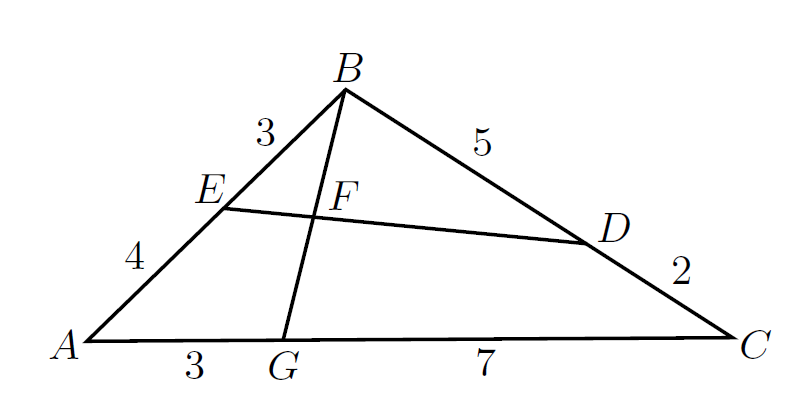
\includegraphics[width=2.5in]{transversal}
	\end{center}
\end{problem}
\begin{problem}
In $\triangle ABC$, point $D$ lies on $\overline{AB}$ such that $\overline{AD}=5$ and $\overline{DB}=2$, and point $E$ lies on $\overline{AC}$ such that $\overline{AE}=3$ and $\overline{EC}=8$. $F$ is the point of intersection of $\overline{BC}$ and the angle bisector of $\angle BAC$, and $G$ is the point of intersection of $\overline{AF}$ and transversal $\overline{DE}$. Find the ratio $AG:GF$. (TJ ARML Practice)
\end{problem}
\subsubsection{Systems}
\begin{problem}
In triangle ABC, points $D$ and $E$ are on sides $BC$ and $CA$, respectively, and points $F$ and $G$ are on side $AB$ with $G$ between $F$ and $B$. $BE$ intersects $CF$ at point $O_1$ and $BE$ intersects $DG$ at point $O_2$. If $FG = 1$, $AE = AF = DB = DC = 2$, and $BG = CE = 3$, compute $\tfrac{O_1O_2}{BE}$.
\end{problem}
\begin{problem}
In a triangle, segments are drawn from one vertex to the trisection points of the opposite side . A median drawn from a second vertex is divided, by these segments, in the continued ratio $x : y : z$. If $x \leq y \leq z$ then find $x : y : z$. (NYSML)
\end{problem}
\subsubsection{Get Creative}
\begin{problem}
In parallelogram $ABCD$, point $M$ is on $\overline{AB}$ so that $\frac {AM}{AB} = \frac {17}{1000}$ and point $N$ is on $\overline{AD}$ so that $\frac {AN}{AD} = \frac {17}{2009}$. Let $P$ be the point of intersection of $\overline{AC}$ and $\overline{MN}$. Find $\frac {AC}{AP}$. (AIME 2009 \#4)
\end{problem}
\begin{problem}
Triangle $ABC$ has $AB=21$, $AC=22$ and $BC=20$. Points $D$ and $E$ are located on $\overline{AB}$ and $\overline{AC}$, respectively, such that $\overline{DE}$ is parallel to $\overline{BC}$ and contains the center of the inscribed circle of triangle $ABC$. Then $DE=m/n$, where $m$ and $n$ are relatively prime positive integers. Find $m+n$. (AIME 2001 \#7)
\end{problem}
\begin{problem}
In triangle $ABC^{}_{}$, $A'$, $B'$, and $C'$ are on the sides $BC$, $AC^{}_{}$, and $AB^{}_{}$, respectively. Given that $AA'$, $BB'$, and $CC'$ are concurrent at the point $O^{}_{}$, and that $\frac{AO^{}_{}}{OA'}+\frac{BO}{OB'}+\frac{CO}{OC'}=92$, find $\frac{AO}{OA'}\cdot \frac{BO}{OB'}\cdot \frac{CO}{OC'}$. (AIME 1992 \#14)
\end{problem}
\newpage 
\section{3D Geometry}
The purpose of this lecture is to introduce some tools for solving 3D geometry problems. Although adding a dimension to 2D seems like it would complicate a lot of things, we actually use much of the same tools we use in 2D, albeit with some different considerations. This lecture is more of a mix of 3D geometry rather than a fixed focus, but that's because I want to introduce you to a lot of topics. This lecture is also more problem-solving based, because the foundation for 3D geometry is actually really simple. It's the application that takes a lot of work getting good at.

\subsection{Coordinate Systems}

In the \textbf{Cartesian Plane}, we are accustomed to denoting a point by a pair of coordinates, usually $(x,y)$.

\begin{figure}[H]
  \centering
  \begin{minipage}[b]{0.4\textwidth}
    \centering
    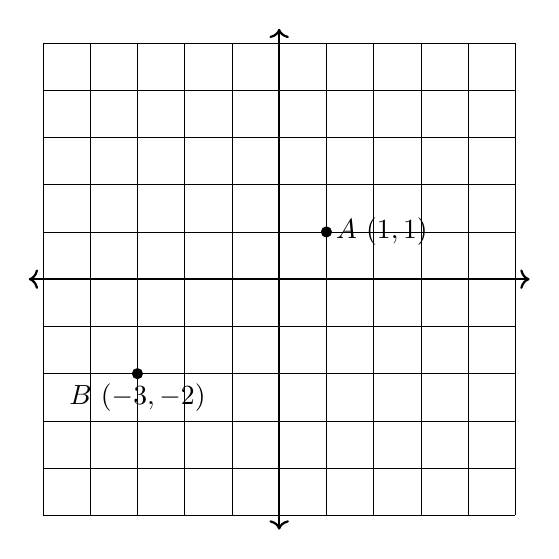
\begin{tikzpicture}[scale=0.6]
    \draw[very thin] (-5,-5) grid (5,5);
    \draw[fill] (1,1) circle [radius=3pt];
    \node[above,right] at (1,1) {$A$ $(1, 1)$};
    \draw[fill] (-3,-2) circle [radius=3pt];
    \node[below] at (-3,-2) {$B$ $(-3, -2)$};
    \draw[<->,thick] (0,-5.3)--(0,5.3);
    \draw[<->,thick] (-5.3,0)--(5.3 ,0);
    \end{tikzpicture}
    \caption{Two points on a Cartesian Plane}
  \end{minipage}
  \hfill
  \begin{minipage}[b]{0.4\textwidth}
    \centering
    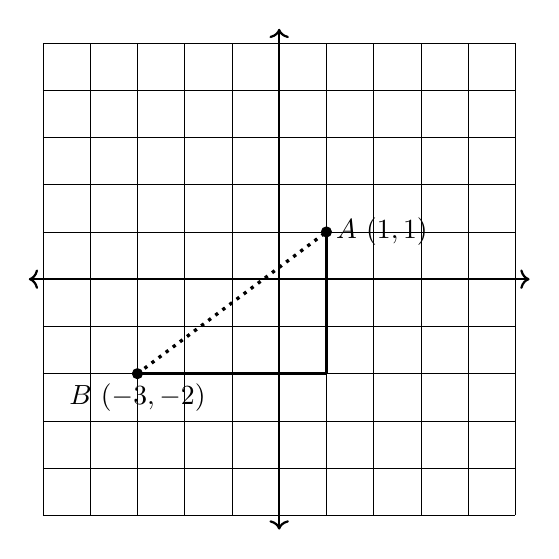
\begin{tikzpicture}[scale=0.6]
    \draw[very thin] (-5,-5) grid (5,5);
    \draw[fill] (1,1) circle [radius=3pt];
    \node[above,right] at (1,1) {$A$ $(1, 1)$};
    \draw[fill] (-3,-2) circle [radius=3pt];
    \node[below] at (-3,-2) {$B$ $(-3, -2)$};
    \draw[<->,thick] (0,-5.3)--(0,5.3);
    \draw[<->,thick] (-5.3,0)--(5.3 ,0);
    \draw[very thick] (-3,-2)--(1,-2);
    \draw[very thick] (1,-2)--(1,1);
    \draw[dotted, very thick] (-3,-2)--(1,1);
    \end{tikzpicture}
    \caption{Use of the Pythagorean Theorem}
    \label{fig:pyth}
  \end{minipage}
\end{figure}

\subsubsection{Distance}

When we want to find the distance between two points, we can employ Pythagorean Theorem as shown in Figure \ref{fig:pyth}. From the right triangle, it is clear that the distance between any points is

$$\abs{\overline{AB}}=\sqrt{\abs{B_x-A_x}^2+\abs{B_y-A_y}^2}$$

Or more commonly written as, given two points $P_1=(x_1,y_1),P_2=(x_2,y_2)$,

\begin{equation}
    \boxed{D(P_1,P_2)=\sqrt{(x_2-x_1)^2+(y_2-y_1)^2}}.
\end{equation}

Note that because of the square of the difference, the order of $x_2-x_1$ does not really matter. I like to think of it as just the absolute value of the two $x$ coordinates squared (because it has to be positive at the end).

\subsubsection{Equation of a Line}

It is important to also introduce the equation of a line in the Cartesian system. There are three forms of the line equation that you have to know. 

\begin{enumerate}
    \item \textbf{Slope Intercept:} $y = mx+b$, where $m=\frac{y_2-y_1}{x_2-x_1}$ is the slope and $b$ is the $y$-intercept (when the line intersects the $y$ axis). This is the most convenient form to have since it tells you so much information.
    \item \textbf{Point-Slope:} $(y-y_1)=m(x-x_1)$, where $m$ is the slope. This form is convenient when you are given two points, because you can easily find the slope and then all you have to do is plug in a point into the equation.
    \item \textbf{Standard Form:} $Ax+By=C$. This is the ``pretty'' form, but doesn't really give us much information, except that you can find the $x$ and $y$-intercepts really easily by setting either one to zero.
\end{enumerate}
%enumerate: Slope intercept, point slope, standard + their advantages

\subsubsection{Coordinate Bashing}
Sometimes when you have no idea what to do for a geometry problem, you can always employ a \textbf{coordinate bash}. Usually, the process goes something like this:
\begin{enumerate}
    \item Write down equations for lines
    \item Find intersections of lines to find desired points
    \item Use distance formula to find distance between points and lengths of line segments
    \item If the problem asks for areas, employ Heron's, determinants, or shoelace 
\end{enumerate}

Note that when you use coordinate bash, you are almost \textit{certainly not using the best method to solve the problem}. Which means that only when you are \textit{desperate} and have time should you consider this method.

\begin{problem}
In $\triangle ABC$, $AB=13,AC=15,BC=14$. Let $E$ be a point on $\overline{AC}$ such that $AE:EC=1:4$, and let $M$ be the midpoint of $\overline{BC}$. Find the length of $\overline{ME}$.
\end{problem}

\subsubsection{Three Dimensions}
First, let's consider the question: what does it mean to be in a higher dimension? Well, to start off, we can easily interpret our lives as a \textbf{3D World}. We have three degrees of freedom of motion that allow us to move and feel 3D textures and all that good stuff. It turns out, we can also think of our world as 4D, because we are also moving through time, another dimension (see how abstract this is getting already?). What all this dimension business means is that each dimension gives us a direction or a \textit{degree of freedom}, something variable that can be changed. 

For our problem-solving purposes, the only definition we are really worried about is \textbf{distance} and how things are positioned relative to each other. It turns out that the Pythagorean Theorem (albeit in a different form) still works for distance in a $n$-dimensional space (you can test this out yourself by applying it twice in 3D). In general, the distance between two points $U$ and $V$ is 

\begin{equation}
    \abs{\overline{UV}} = \sqrt{\sum\limits_{i=1}^{n} (v_i-u_i)^2}
\end{equation}

Since 3D is the most common higher-dimensional geometry you'll see in competition math, the distance equation (for convenience) is

\begin{equation}
    \boxed{\abs{\overline{UV}} = \sqrt{\sum\limits_{i=1}^{3} (v_i-u_i)^2}= \sqrt{(v_1-u_1)^2+(v_2-u_2)^2+(v_3-u_3)^2}}
\end{equation}

\subsection{3D Geometry Problem-Solving Strategies}
In 3D problems, we often reduce down to 2D problems because we know how to deal with those later. As an example, consider this problem:

\begin{problem}
Find the surface area and volume of a tetrahedron with side $s$.
\begin{center}
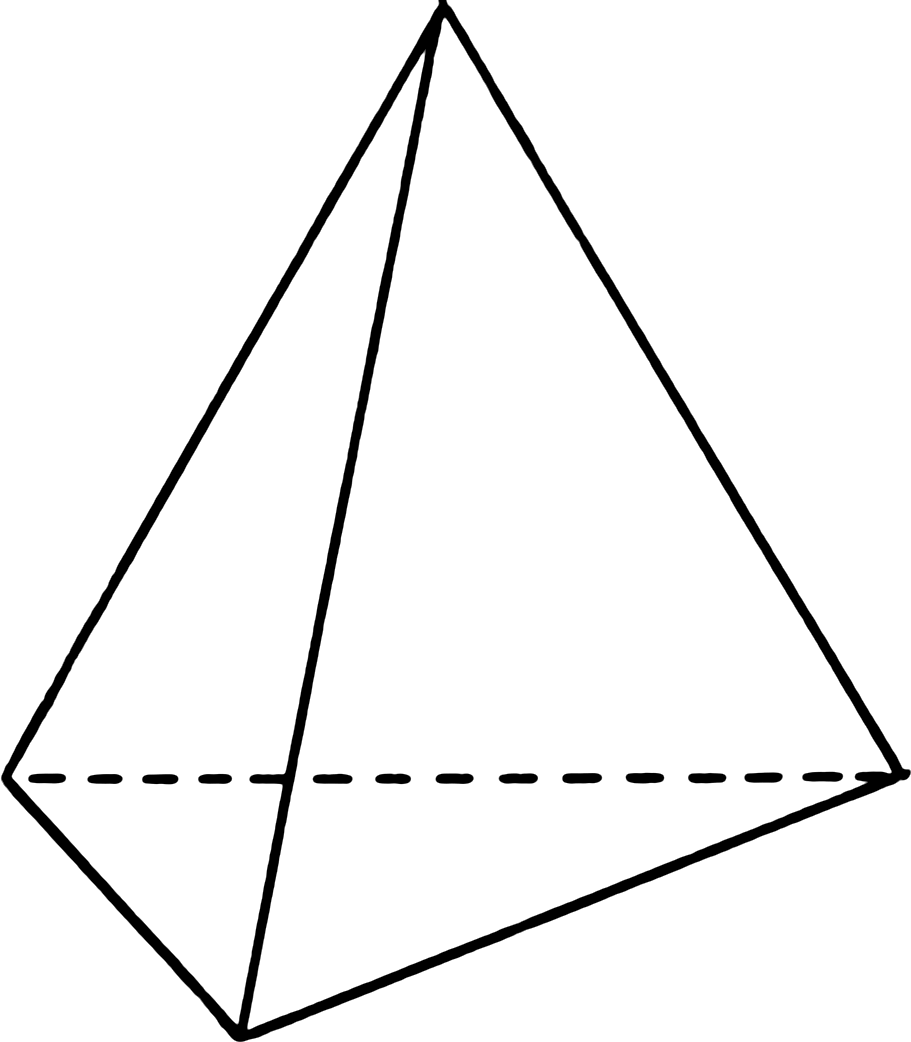
\includegraphics[width = 1.2in]{tetra}
\end{center}
\end{problem}

\textbf{Solution:}
We know the area of an equilateral triangle with side $s$ is just

$$\frac{s^2\sqrt{3}}{4}.$$

Now we just need to find the height from the base of the tetrahedron to the top vertex. This easy to do once we view the tetrahedron from the top vertex, because we find out that the top vertex height drops directly down to the center of the equilateral triangle. We can then use one of the edges and the distance from the center of the equilateral triangle to one of its sides along with the height to build a right triangle. The height is then just 
$$\sqrt{s^2-\left(\frac{s}{\sqrt{3}}\right)^2}=s\sqrt{\frac{2}{3}}$$
and the volume is 
$$\frac{1}{3}\cdot s\sqrt{\frac{2}{3}}\cdot \frac{s^2\sqrt{3}}{4} = \boxed{\frac{s^3\sqrt{2}}{12}}$$
DON'T ever forget the $\frac{1}{3}$ factor for the volume of pyramids.

As you can see, 3D geometry problems are really just a bunch of 2D problems, so whenever you have a 3D object, try to dissect it down as much as possible! Try looking at the object in different perspectives, chopping it up, and drawing in extra lines. Also, sometimes the 3D geometry problem is just a setup for an algebra problem. Unfortunately, this algebra can sometimes get \textit{very ugly}. But what can you do? Math all relies on each other, and pure geometry can't always get you to the final answer.


\subsection{Euler's Formula} %https://www.artofproblemsolving.com/wiki/index.php?title=Euler%27s_Polyhedral_Formula
Euler's Formula states that 
\begin{equation}
    F+V-E=2,
\end{equation}
where $F$ is the number of faces, $V$ is the number of vertices, and $E$ is the number of edges.

\begin{problem}
Fill in the following table to verify Euler's Formula

\begin{figure}[H]
    
  \begin{minipage}[]{0.24\textwidth}
    \centering
    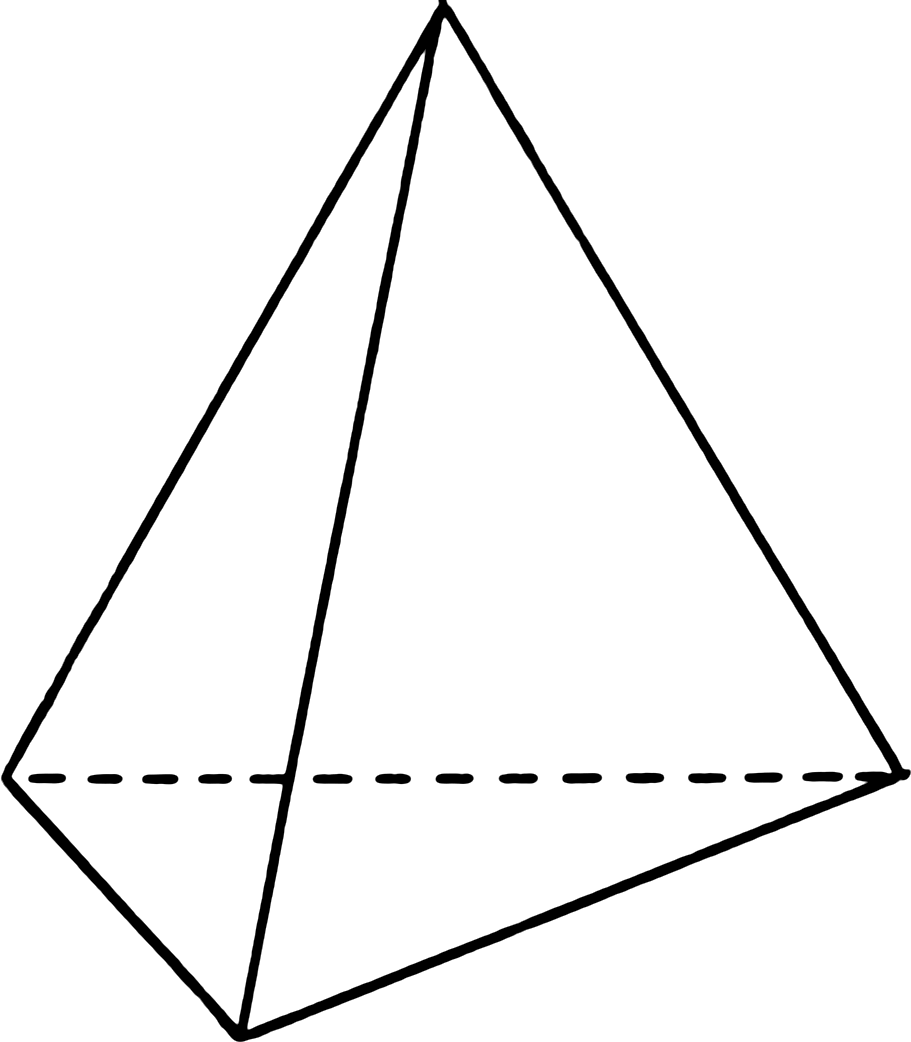
\includegraphics[width = 1.2in]{tetra}
    \caption{Tetrahedron}
    \label{fig:tetra}
  \end{minipage}
  \begin{minipage}[]{0.22\textwidth}
    \centering
    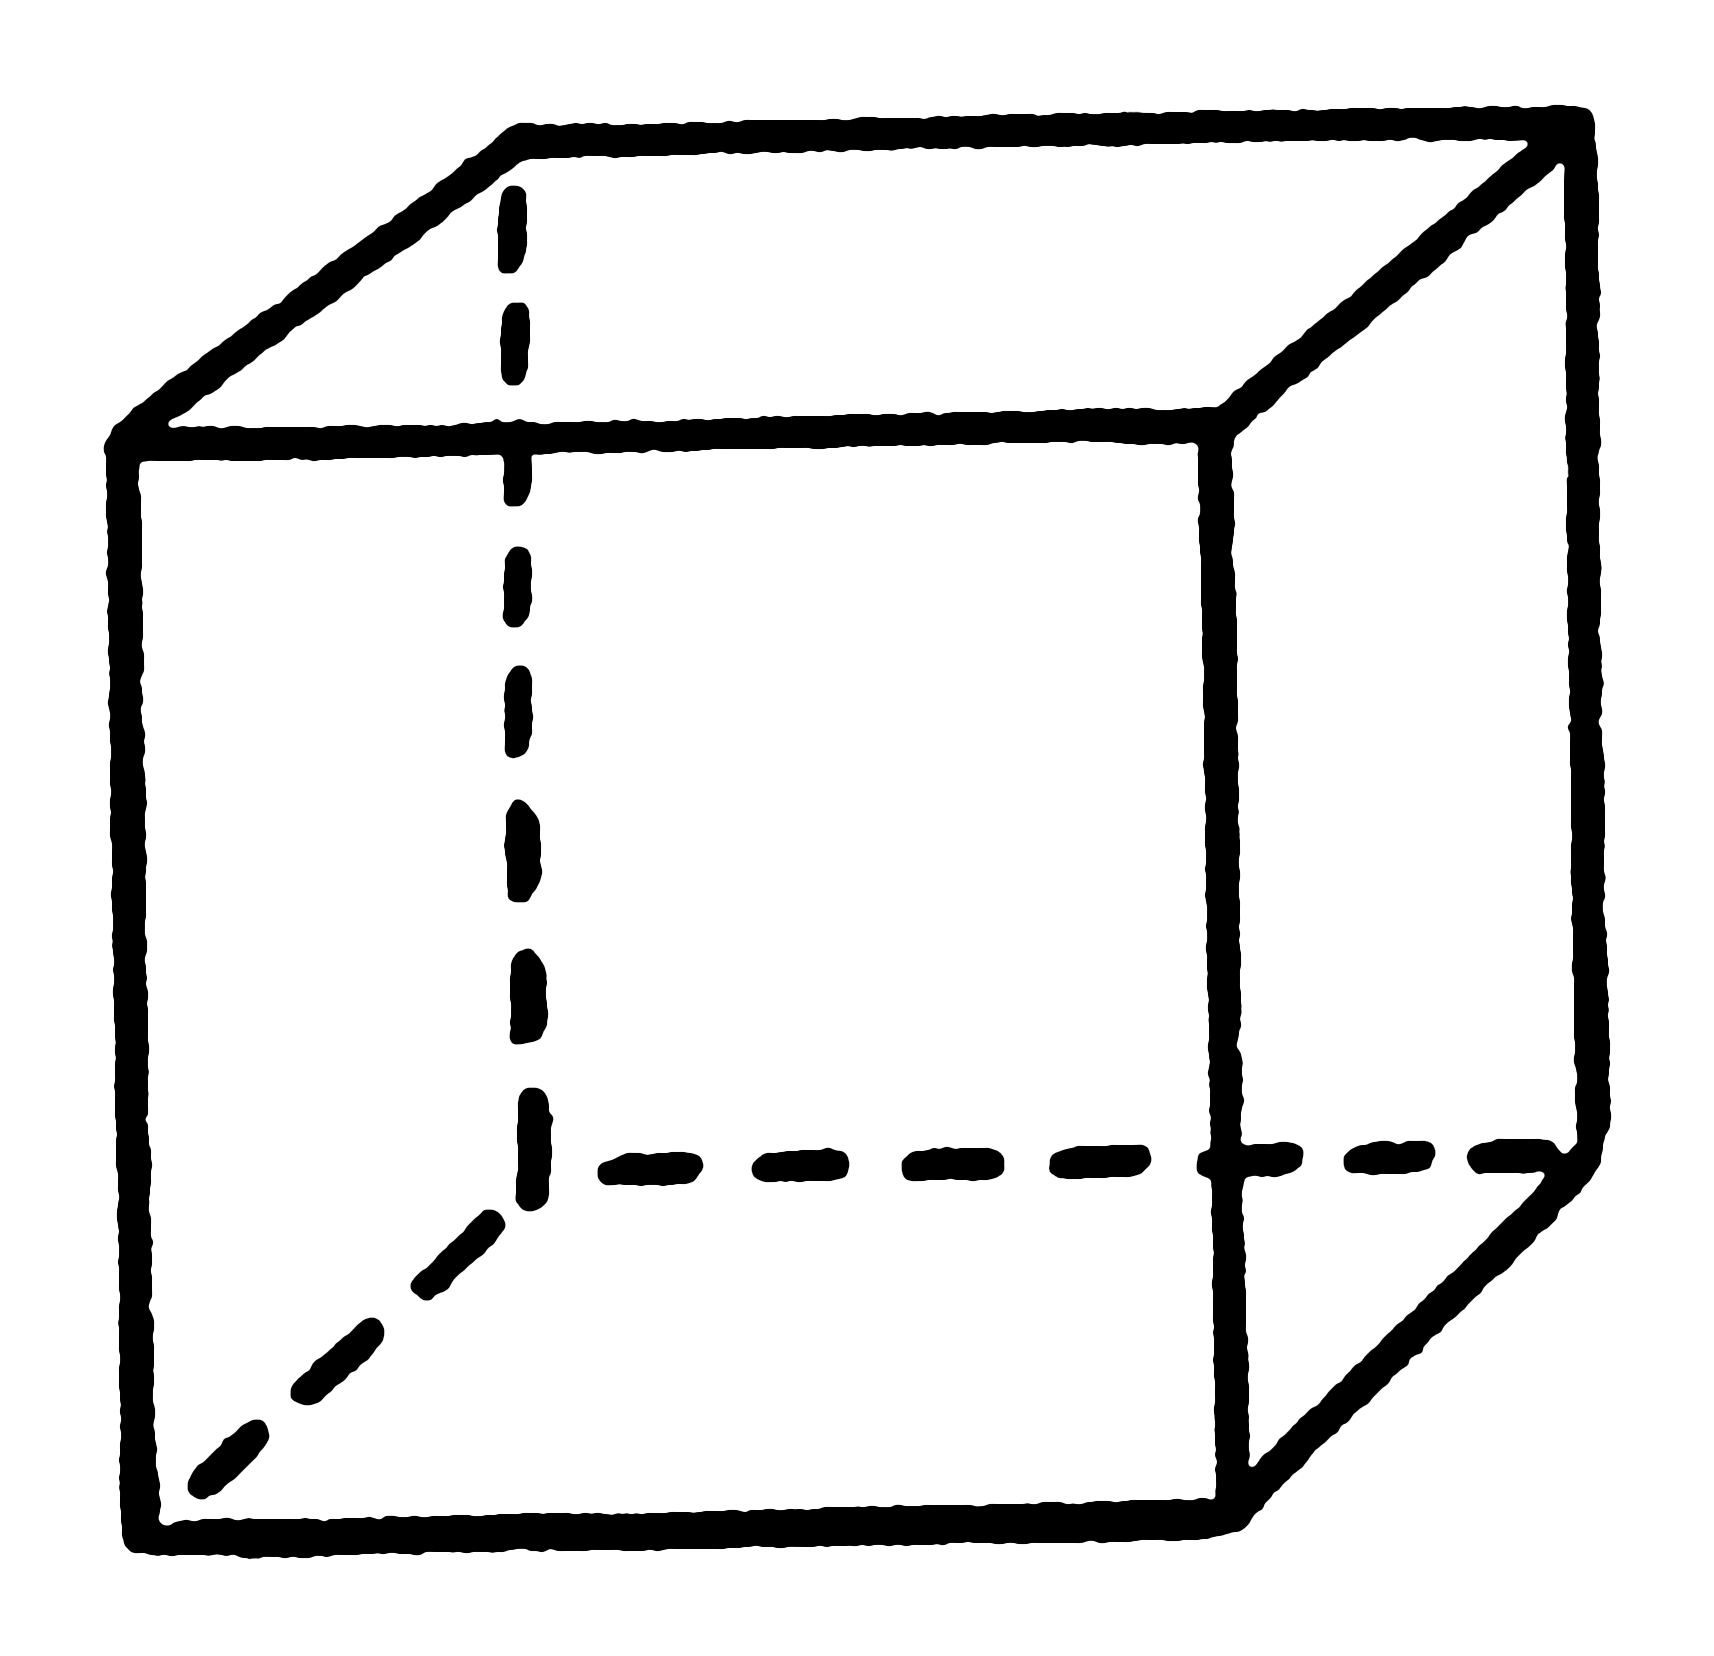
\includegraphics[width=1.4in]{cube2}
    \caption{Cube}
    \label{fig:cube}
  \end{minipage}
  \begin{minipage}[]{0.25\textwidth}
    \centering
    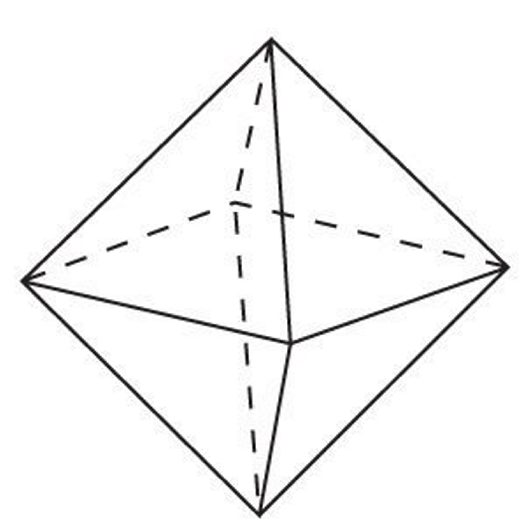
\includegraphics[width = 1.37in]{octa}
    \caption{Octahedron}
    \label{fig:octa}
  \end{minipage}
  \begin{minipage}[]{0.25\textwidth}
    \centering
    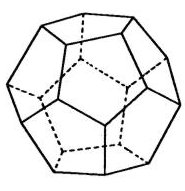
\includegraphics[width=1.35in]{dodec2}
    \caption{Dodecahedron}
    \label{fig:dodec}
  \end{minipage}
  
\end{figure}

\centering
\def\arraystretch{1.5}
$\begin{tabular}{|c|c|c|c|}\hline Shape & Vertices & Edges & Faces\\ 
\hline Tetrahedron &  & &  \\ 
\hline Cube &  &  & \\ 
\hline Octahedron &  &  & \\ 
\hline Dodecahedron & &  & \\ 
\hline 
\end{tabular}$
\end{problem}

\subsection{Problems}
%https://artofproblemsolving.com/wiki/index.php?title=Category:3D_Geometry_Problems

\begin{problem}
Find the equation of the line that passes through $(4, 5)$ and $(-11, 18)$ and find its slope and $y$-intercept.
\end{problem}

\begin{problem}
Find the distance between:
\begin{itemize}
    \item $(1,-10)$ and $(9,5)$
    \item $(3,-10)$ and $(19,-4)$
    \item $(2,-4,11)$ and $(7,6,-3)$
    \item $(1, 3, 2, -6, 7, 8)$ and $(-4, 4, 2, 4, 7, 11)$
\end{itemize}
\end{problem}

\begin{problem}
Find the surface area and volume of an octahedron with side $s$.
\begin{center}
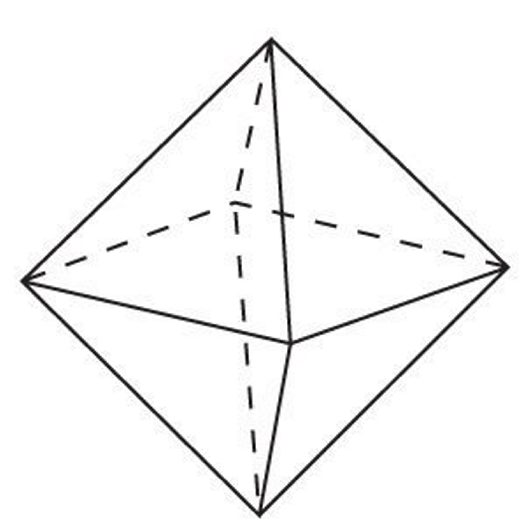
\includegraphics[width = 1.37in]{octa}
\end{center}
\end{problem}

\begin{problem}
The edges of a cube sum up to 144. What is the length of its spacial diagonal? \textit{Source: MATHCOUNTS}
\end{problem}

\begin{problem}
The surface area of a cube is twice its volume. Find the interior diagonal of the cube. \textit{Source: MATHCOUNTS}
\end{problem}

\begin{problem}
A cube is inscribed in a sphere, find the ratio of the volume of the cube to the sphere.
\end{problem}

\begin{problem}
A $5\times 8$ rectangle can be rolled up into a cylinder in two different ways. Find the ratio of the more voluminous cylinder to the smaller one. \textit{Source: MATHCOUNTS}
\end{problem}

\begin{problem}
A rope is wrapped exactly five times around a cylinder of radius 3 and height 20. What is the length of the rope?
\end{problem}

\begin{problem}
A right prism with height $h$ has bases that are regular hexagons with sides of length $12$. A vertex $A$ of the prism and its three adjacent vertices are the vertices of a triangular pyramid. The dihedral angle (the angle between the two planes) formed by the face of the pyramid that lies in a base of the prism and the face of the pyramid that does not contain $A$ measures $60$ degrees. Find $h^2$. \textit{Source: AIME}
\end{problem}

\begin{problem}
Buildoo is designing a new shape of brick. He constructs it by setting a brick cone with slant height 5 and base radius 4 on the ground, then cutting off a smaller cone with a cut parallel to the base of the cone (this forms a frustum). If the volume of Buildoo’s brick is $\frac{63\pi}{4}$, what is its surface area? \textit{Source: TJTST}
\end{problem}

\begin{problem}
A rectangular box has integer edge lengths. The sum of the numerical values of its volume, its surface area, and its twelve edge lenghths is 2015. Compute the length of the box's interior diagonal. \textit{Source: ARML}
\end{problem}

\begin{problem}
Corners are sliced off a unit cube so that the six faces each become regular octagons. What is the total volume of the removed tetrahedra?
\vspace{0.1in}
\begin{figure}[H]
    \centering
    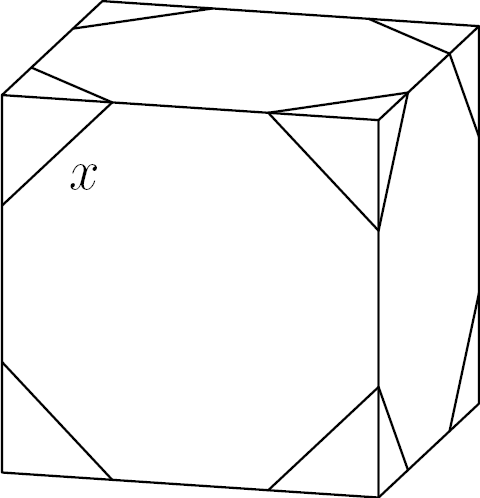
\includegraphics[width=1.7in]{cubetetra}
    \caption{Diagram for Problem \ref{pr:cubetetra}}
\end{figure}
\label{pr:cubetetra}
\end{problem}

\begin{problem}
Three mutually tangent spheres of radius $1$ rest on a horizontal plane. A sphere of radius $2$ rests on them. What is the distance from the plane to the top of the larger sphere? \textit{Source: AMC}
\end{problem}

\begin{problem}
Six spheres of radius $1$ are positioned so that their centers are at the vertices of a regular hexagon of side length $2$. The six spheres are internally tangent to a larger sphere whose center is the center of the hexagon. An eighth sphere is externally tangent to the six smaller spheres and internally tangent to the larger sphere. What is the radius of this eighth sphere? \textit{Source: AMC}
\end{problem}

\begin{problem}
Let $ABCD$ be a unit square. Let $E$ be the midpoint of $\overline{AB}$ and let $F$ be the midpoint of $\overline{BC}$. Find the area of the triangle bounded by the lines $\overline{EC}, \overline{AF}$, and $\overline{DF}$
\end{problem}

\chapter{Applications}
\section{Game Theory}
When we talk about games, we usually concern ourselves with the question of \textit{how do I maximize my winnings}? \textbf{Game Theory} is a topic that analyzes exactly how to do this, digging into the structure of games and the behavior of players. Obviously, since game theory is such a large topic, we will only brush the surface of the subject, but will take a look at both one and two-player games. We will see that because of how well game theory describes human behavior, we will be able to use it to look at a real-world application.


\subsection{Expected Value}
Expected Value is exactly what it sounds like---the expected outcome of some sort of event.

\begin{definition}
The \textbf{Expected Value}, denoted $E$ (or $\mu$), is 

\begin{equation}
    E = \sum\limits_{i=1}^{n} p_i x_i = p_1x_1+p_2x_2+p_3x_3+\cdots+p_nx_n,
\end{equation}
where $x_i$ is the value of the event that occurs with probability $p_i$.
\end{definition}

\subsection{One-Player Games}
To get an intuition of expected value, we look at this simple game:

\begin{problem}
Suppose we play a game so that each time you roll a standard dice, you win the amount of dollars that you roll. What is the expected amount of dollars you win every roll?
\end{problem}

To solve this problem, we need to figure out our probabilities and values of events. Clearly, each event has a $\frac{1}{6}$ chance of happening, and the events are $\{\$1,\$2,\$3,\$4,\$5,\$6\}$. Therefore, our expected value is

$$E = \frac{1}{6}(\$1+\$2+\$3+\$4+\$5+\$6)=\boxed{\$3.50}$$

It is important to note that when people make games and charge you for playing, they usually make these expected value computations. For example, in our previous problem, since you expect to win $\$3.50$, the person who runs the game will obviously want you to pay more per game, and will likely charge you a higher price to play. 

It is also interesting to note that the expected value of a game is not always the most likely outcome. For example, $\$3.50$ isn't even a possible outcome of our dice game. However, if you play the game over and over again many times, you should find that this dollar amount is your average winnings.

\subsubsection{Monty Hall}
There is this popular game show that is played like the following. Suppose we have three curtains, 

\begin{itemize}
    \item Two curtains have goats behind them
    \item One curtain has a car behind it
\end{itemize}

The goal of the game is to choose the curtain with the car behind it to win it. We begin the game by having the contestant pick a curtain. Then, the host reveals to the contestant which one of the remaining two curtains has the goat. Now, with two curtains left, the host asks the contestant,
\begin{center}
``Do you want to switch to the other curtain, or keep your own?''
\end{center}

\begin{problem}
In this game show, should the contestant switch?
\end{problem}

This game show problem is known as the \textbf{Monty Hall Problem}, named after the host of the original TV show that introduced it. If you are still skeptical about the problem, you aren't alone! In fact, when this problem debuted in the \textit{New York Times} in 1991, a huge debate broke out between high-profile mathematicians. However, with our probabilistic methods, we can determine the answer to the Monty Hall Problem.

\subsection{Two-Player Games}
Now that we have conquered one-player games, we turn to two-player games. Here is where game theory really gets cool (and complicated at the same time). When you have more than one player, \textit{everybody wants to maximize their benefits}. This underlying assumption is what builds everything for game theory---we need to not only consider what we do, but what other people want to do.

\subsubsection{Tony's Accident\protect\footnote{This section is adapted from ``Introduction to Game Theory'', by S. Schecter and H. Gintis}}

Our first example deals with a scenario where Tony and Steve have gotten into a minor traffic accident. Steve is the victim, who is complaining about some scratches on his car. Normally, I would write out the descriptions of all the scenarios, but to save yourself time and to illustrate how to handle this problem, I will introduce the \textbf{game tree} for this problem:

\begin{center}
\begin{forest}
[Tony
    [Sends \$80[Steve pockets money[(\$-80{,} \$80)]]]
    [Sends \$40[Steve repairs[(\$-80{,} \$20)]] [Steve doesn't repair[(\$-40{,} \$40)]] ]
    [Asks for Receipt [Steve repairs[(\$-80{,} \$20)]] [Steve doesn't repair[(\$0{,} \$0)]] ]
]
\end{forest}
\end{center}

When we look at the tree, we see a \textbf{root}, or the starting point, \textbf{nodes} that denote scenarios, and \textbf{terminal nodes} that represent \textbf{payoffs}, e.g. (\$-80{,} \$80); the payoff is read in this case as the first number denoting Tony's winnings and the second number denoting Steve's winnings---(\$-80{,} \$20) would represent Tony losing \$80 and Steve winning \$20. The tree describes the game and its moves perfectly, Tony has three options at the start, to pay Steve the full bill of the repairs, \$80, and let Steve decide what he wants to do with it. Since Steve only gains \$20 of happiness from the repairs, if he uses the \$80 for the repairs, he only gains that amount (while Tony loses \$80); this is the payoff described by (\$-80{,} \$20). You can similarly deduce the scenarios by choosing different paths down the tree. There are several theorems you can learn about trees and nodes, such as the path uniqueness of reaching any node on a tree like such, but that is beyond the scope of this lesson (and although are useful to prove, the proof itself isn't that useful). We instead look to solve this problem, 

\begin{problem}
What is Tony's best strategy, and what outcome does it lead to?
\end{problem}

When we solve this problem, we have to keep in mind that \textit{the result depends on the choices of everybody}. What we could do is work our way from top to bottom, visiting every scenario and figuring out what happens, but this is inefficient and very hard to do with big trees. Instead, we do something called \textbf{backwards induction}, which has the following procedures.

\textbf{Backwards Induction:}
\begin{enumerate}
    \item Begin at a node $c$ that leads to only terminal nodes
    \item For whoever's turn it is, determine which node the player will take
    \item Cross out the ones that will never happen
    \item Assign the payoff that was chosen to be the payoff of $c$
    \item Keep working your way up, repeating this process over and over again
\end{enumerate}

Using this method, our first iteration will lead to the tree:
\begin{center}
\begin{forest}
[Tony
    [Sends \$80[(\$-80{,} \$80)]]
    [Sends \$40[(\$-40{,} \$40)]]
    [Asks for Receipt [(\$-80{,} \$20)]] ]
]
\end{forest}
\end{center}

And one more iteration will make it obvious that Tony's best move is to send \$40, since this will lead to a loss of only \$40, as opposed to \$80.

From our analysis, we see that we can't always get to the best solution for both players. For example, you could argue that (\$0, \$0) is the best for everyone, since nothing happens, but clearly Steve will not let this be the final result. 

It is also important to note before we end this section that backward induction fails if we have the following scenario

\begin{center}
\begin{forest}
[Person 1
    [(\$20{, }\$-30)]
    [(\$20{, }\$-40)]
]
\end{forest}
\end{center}

As you can see, Person 1 doesn't really care what option he/she chooses, the result is always a gain of \$20. However, I guess if you think Player 1 wants to hurt Player 2, then he/she will choose to be mean and force the \$-40, the worse option, on Player 2. Just remember that in game theory, we usually treat this case as \textit{indeterminate}.

\subsection{Prisoner's Dilemma}
A very popular two-player game is played like the following. Consider the scenario that two people are captured for their crimes. The police then separate the two criminals, and give them the following options, to confess to the crime and rat out on their partner, or to just keep quiet and not have evidence that the criminals did the crime. Here are the following possibilities, displayed as a \textbf{payoff matrix}.

\begin{center}
\renewcommand{\arraystretch}{1.5} % Default value: 1
\begin{tabular}{cc|c|c}
     &\multicolumn{3}{c}{Person A} \\
     && Confess & Keep Quiet \\
     \cline{2-4}
     \multirow{2}{*}{Person B}&Confess & 10 yrs, 10 yrs & 0 yrs, 20 yrs \\
     &Keep Quiet & 20 yrs, 0 yrs & 5 yrs, 5 yrs
\end{tabular}
\end{center}

Note that the payoffs are written in the order so that the first number corresponds to the person on the left of the table. We see that if they both confess, they both take 10 yrs in prison. If only one person rats out their partner, then the police will let the confess-er leave for free and instead put the full penalty on the partner. If both stay quiet, police can only set their sentence to 5 yrs in prison.

The question now is, what should each player do, and what actually happens at the end?

This problem is famously known as the \textbf{Prisoner's Dilemma}. The formal terms we use for the game are that each player moves according to their \textbf{dominant strategy}, which might not always exist, and the final result is known as the \textbf{Nash Equilibrium}, which may not always exist either.

\subsubsection{Economics}
The most well-known application of the prisoner's dilemma is in economics, specifically in oligopolies, which are industries that are controlled largely by a few companies (think soda (Pepsi, Coke) or oil (Exxon, Shell)). The reason this problem occurs is that the government prevents \textbf{collusion}, which is the secret agreement between companies to maximize their profits, so companies don't know what each other are going to do. The other reason is that companies \textbf{cheat}, that is, even if companies come to an agreement, people have an incentive to break the agreement to maximize their own profits. Enough with the economics, let's just do a typical oligopoly problem.

\begin{problem}
Suppose Exxon and Texaco are faced with the following decision, they can either drill one or two new wells to expand their company's production. However, if both companies choose to drill two wells, there is too high of a supply of oil, and prices will drop, leading to less profit earned. If one of the companies decides not to drill a second well, then the company that has two wells will benefit from more sales. We can see this in the payoff matrix:

\begin{center}
\renewcommand{\arraystretch}{1.5} % Default value: 1
\begin{tabular}{cc|c|c}
     &\multicolumn{3}{c}{Exxon} \\
     && Drill Two & Drill One \\
     \cline{2-4}
     \multirow{2}{*}{Texaco}&Drill Two & \$4 million, \$4 million & \$6 million, \$3 million \\
     &Drill One & \$3 million, \$6 million & \$5 million, \$5 million
\end{tabular}
\end{center}
\end{problem}

Determine each company's \textbf{dominant strategy}, and the \textbf{Nash equilibrium}.

\subsection{Problems}
\begin{problem}
Suppose I have a bag of 12 slips of paper in it. Some of the slips have the number 2 on them and the rest of 7. If the expected value of the number shown on a random slip drawn is 3.25, compute the number of 2-slips and 7-slips.
\end{problem}

\begin{problem}
Suppose we have a rigged dice so that the probabilities of rolling a number $n$ is $\frac{n}{21}$. If you win the amount that you roll, what is your expected winnings of a single roll?
\end{problem}

\begin{problem}
Perhaps a better way to remove the skepticism with the Monty Hall problem is to consider it in a bigger case. Suppose there are 100 curtains---99 goats and one car. After you choose a curtain, the host removes 98 of the curtains, leaving you with the choice of switching or keeping your curtain. What would you do?
\end{problem}

\begin{problem}
Let's say we have another Monty Hall like game. Except now, there are 4 curtains, 3 goats and 1 car behind the curtains. On each turn, the host reveals a goat, and gives you the option of switching curtains. What is your best strategy to win the car?
\end{problem}

\begin{problem}
Pepsi and Coca-Cola are deciding whether or not to increase their advertising campaign. Their payoff matrix is described by the following:

\begin{center}
\renewcommand{\arraystretch}{1.5} % Default value: 1
\begin{tabular}{cc|c|c}
     &\multicolumn{3}{c}{Pepsi} \\
     && Many Ads & Few Ads \\
     \cline{2-4}
     \multirow{2}{*}{Coke}&Many Ads & \$25 million, \$25 million & \$70 million, \$10 million \\
     &Few Ads & \$10 million, \$70 million & \$40 million, \$40 million
\end{tabular}
\end{center}

Determine the \textbf{dominant strategy} for each company and the \textbf{Nash equilibrium}.
\end{problem}

\begin{problem}
Little Kona is a small coffee company that is considering entering a market dominanted by Big Brew. Each company's profit depends on whether Little Kona enters and whether Big Brew sets a high or a low price:

\begin{center}
\renewcommand{\arraystretch}{1.5} % Default value: 1
\begin{tabular}{cc|c|c}
     &\multicolumn{3}{c}{Big Brew} \\
     && High Price & Low Price \\
     \cline{2-4}
     \multirow{2}{*}{Little Kona}&Enter & \$2 million, \$3 million & \$-1 million, \$1 million \\
     &Don't Enter & \$0 million, \$7 million & \$0 million, \$2 million
\end{tabular}
\end{center}

\begin{enumerate}[label=\alph*)]
    \item What is Little Kona's dominant strategy?
    \item What is Big Brew's dominant strategy?
    \item What is the Nash equilibrium?
    \item Big Brew threatens Little Kona that ``if you enter, we will set a low price and you will lose money.'' Should Little Kona believe Big Brew's threats and stay out?
\end{enumerate}
\end{problem}

\begin{problem}
Suppose you accidentally run over your friend's lawn with your car. You need to determine what course of action to minimize your losses. The game tree is displayed below:

\begin{center}
\begin{forest}
[You
    [Send \$1000[Friend repairs[(\$-1000{,} \$1000)]] [Friend asks for help[(\$-2000{,} \$1500)]]]
    [Offers Help [Friend takes help[(\$-1500{,} \$1500)]] [Friend denies help but wants money[(\$-1000{,} \$1000)]] ]
]
\end{forest}
\end{center}
\end{problem}

What should be your course of action?

\chapter{Chemistry}
\section{Stoichiometry}
Stoichiometry is one of the most important skills you need in chemistry, because chemistry is the study of reactions and...well...stoichiometry is the math of reactions. 

\subsection{Introduction}
Let us begin by talking about the story of the Jellybean Shop. Long ago, in the 1970s, candy used to be cheap. Kids used to be able to go into stores with a nickel and come out with a bag full of candy. However, for the shopkeeper, this was no fun business. Kids often asked for 50, 100, even 1000 jellybeans...and the shopkeeper had to count the jelly beans one by one so the kids wouldn't feel like they were getting cheated out. 

One day, the shopkeeper decided that he had to change his ways. He could no longer just count jellybeans one by one---he had to find a faster way. So in his shop, he started weighing individual jellybeans, and he created the following data table.
\begin{center}
\begin{tabular}{|c|c|}
    \hline
     Bean 1 & 0.95 g \\
     Bean 2 & 1.00 g \\
     Bean 3 & 0.98 g \\
     Bean 4 & 0.99 g \\
     Bean 5 & 1.02 g \\
     Bean 6 & 1.01 g \\
     Bean 7 & 0.99 g \\
     Bean 8 & 1.00 g \\
     Bean 9 & 1.03 g \\
     Bean 10 & 1.00 g \\
     \hline
\end{tabular} 
\end{center}
Wow! It turns out that the jellybeans all had a similar mass. The 10 jellybeans he weighed averaged to a mass of 1.003 g/jellybean. Ever since this discovery, the shopkeeper's life has been a lot easier. No longer does he have to labor over counting thousands of jellybeans everyday...one by one. Now, he knows that all he has to do is weigh the mass of jellybeans to determine how many there are. For example, if someone asks for 4729 jellybeans, all he has to do is weigh out:
$$4729 \text{ jellybeans} \times \frac{1.003 \text{ g}}{1 \text{ jellybean}} = \boxed{4743.187 \text{ grams}},$$
or about 4.7 kg. 

At this point, you might be wondering. How does jellybeans have to do with stoichiometry...or even chemistry? Well let me give you a new problem. Suppose I wanted you to figure out how many molecules of oxygen you had in the air, or how many gold atoms were in a bar of gold. Would you grab a super microscope and count all of the atoms and molecules? I hope not.

\subsection{Atomic Mass}
Here we introduce the concept of atomic mass. Just like jellybeans, chemists have so nicely weighed out the masses of atoms and found their average. So the \textbf{atomic mass} of an element is the average mass of an atom. Basically, if you were to measure the masses of a lot of atoms (like a million), their average mass would be the atomic mass. There are complicated reasons why atomic masses aren't perfect (it has to do with isotopes), but we can save that discussion for another day. 

Now let's look at a part of the periodic table to familiarize ourselves with the atomic mass:
\begin{center}
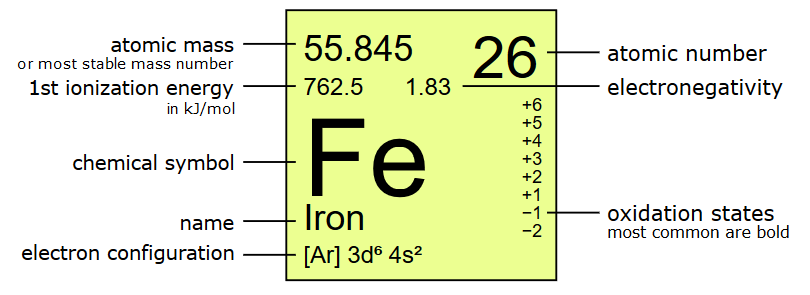
\includegraphics[width=4in]{feLabel}
\end{center}
As you can see, the atomic mass of Fe, or iron, is about 55.85. But what are the units? Grams? No way, one atom of iron is definitely not that heavy. On the periodic table, the units for this mass is 55.85 grams/mole, where the mole is $6.022 \times 10^{23}$ atoms. The \textbf{mole} is defined as the number of carbon atoms in exactly 12 grams of pure carbon-12. For our purposes, the mole is just a big number that helps us make calculations on a reasonable scale. To reinforce what we just learned about jellybeans and atomic mass, let's do a simple problem. 

\begin{problem}
I am told I have a bar of pure gold that has a mass of 4 grams. How many gold atoms are in this bar? 
\end{problem}
\begin{solution}
We begin by identifying the atomic mass of gold, or Au, and find that it is: 196.97 grams/mole. \par
Then, we just divide 4 grams by this atomic mass to figure out the number of moles of gold:
$$4 \text{ g} \times \frac{1 \text{ mol}}{196.97\text{ grams}} = 0.0203 \text{ mole}.$$
And since we know that 1 mole = $6.022 \times 10^{23}$ atoms, 
$$0.0203 \text{ mol} \times \frac{6.022 \times 10^{23} \text{ atoms}}{1 \text{ mole}} = \boxed{1.22 \times 10^{22} \text{ gold atoms}}.$$
That a lot of atoms! This really shows you how small atoms are.
\end{solution}
\begin{problem}
My lab adviser wants me to calculate the number of oxygen atoms in a container that holds 0.800 kg of pure oxygen.
\end{problem}
\begin{problem}
My friend claims that he can life up $1.12\times10^{27}$ atoms of pure silver. Should I believe him?
\end{problem}
\begin{problem}
What is the mass of 1.73 moles of carbon?
\end{problem}

\subsection{Molar Mass}
Ok, so molar mass isn't actually that much different from atomic mass. In fact, if you literally took the definition of atomic mass and replaced ``atom'' with ``molecule'', you'd have the new definition. So here is the definition of \textbf{molar mass}:\textit{the mass of one mole of a compound, also known as molecular mass}. Let's do some problems:

\begin{problem}
Glucose, or \ce{C_6H_{12}O_6} is a very important biological molecule. Calculate its molar mass.
\end{problem}
\begin{problem}
Magnesium Sulfate (\ce{MgSO_4}), also known as Epsom salts, is often used in baths to help sooth sore muscles. If I dump 1 kg of it into my bat, how many moles of \ce{MgSO_4} am I dumping in?
\end{problem}
\begin{problem}
Calculate the percentage masses of each atom in glucose (\ce{C_6H_{12}O_6}).
\end{problem}
\begin{problem}
We now introduce the problem of determining the molecular formula of a compound given its percent compositions. For example, given that a compound has the following:
$$71.65\% \ce{ Cl} \quad 24.27 \% \ce{ C} \quad 4.07 \% \ce{ H},$$
and has a molar mass of 98.96 g/mol, find the empirical and molecular formulas.
\end{problem}
\begin{solution}
We first want to convert the percentage of the elements into masses, and then moles. We find this to be 71.65 g of chlorine, 24.27 g of carbon, and 4.07 g of hydrogen. Now we can calculate the \textit{mole ratio}, by figuring out the proportionate moles of these atoms:
\begin{center}
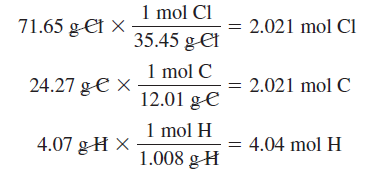
\includegraphics[width=2.5in]{chemEq}
\end{center}
Now we figure out the \textbf{empirical formula}, which is the ratio of atoms in their most simplified form, which means the greatest common factor of the atom ratios is 1. We can do this by dividing our mole ratios by the lowest number, so no we have 
\begin{center}
\begin{tabular}{c|c}
    
    Cl & 1 \\
    C & 1 \\
    H & 2 \\
    
\end{tabular}
\end{center}
So we see that our empirical formula is \ce{ClCH2}. To figure out the molecular formula, we just need to figure out how many molar masses of this empirical formula go into the molecular mass. This is easy because:
$$\frac{\text{Molar mass}}{\text{Empirical formula mass}} = \frac{98.96 \text{ g/mol}}{49.48 \text{ g/mol}} = 2$$
So our final molecular formula is $\boxed{\ce{Cl2C2H4}}$.
\end{solution}
\begin{problem}
A white powder is found to have 43.64 \% phosphorus and 56.36 \% oxygen by mass. If the compound has a molar mass of 283.66 g/mol, what are the empirical and molecular masses of this compound?
\end{problem}
\begin{problem}
Caffeine, a stimulant found in coffee, tea, and chocolate, contains 49.48 \% carbon, 5.15 \% hydrogen, 28.87 \% nitrogen, and 16.49 \% oxygen by mass and has a molar mss of 194.2 g/mol. Determine the molecular formula of caffeine.
\end{problem}
\subsection{Chemical Equations}
Now comes the crux of the power of stoiciometry, chemical equations. Let us start with a simple reaction:
$$\ce{CH4 + 2O2 -> CO2 + 2H2O}$$
On the left hand of the $\rightarrow$, we have the \textbf{reactants}, and on the right side, the \textbf{products}. What this equation tells us is that this reaction takes in the reactants and through a chemical process, makes products. Notice that this equation is \textit{balanced}, that is, the number of atoms on each side are equal. For example, in this one both sides have 1 C, 4 H, and 4 O. \par
Although reactions are a primary part of chemistry, I won't be able to go over all of them in this lecture. I will take liberty and instead talk about doing the equation problems rather than talking about the theory and background of the reactions. This way, you'll be able to do more problems (theory is good but this is an introductory class after all). If you want to learn about reactions, there are plenty of good textbooks out there that can help you. \par
\subsubsection{Balancing Equations}
The first thing we need to do about equations is learn how to balance them. Even though an unbalanced equation tells us what reaction is occurring, if an equation is not balanced, we will not be able to do math with it. \par
As I mentioned earlier, a balanced equation has the same numbers of each atom on each side of the equation. Although there is a systematic way to balance equations, it requires linear algebra (which I imagine would be well beyond what most of you guys have learned so far). Using the trial and error method is pretty strong and fast (much faster than the matrix method) anyway, so let's learn that. \par
Let us start with an equation:
$$\ce{C2H5OH + O2 -> CO2 + H2O}$$
Just FYI, this is an equation representing the reaction between ethanol and oxygen, which produces carbon dioxide and water. The first thing we notice about this equation is that it is clearly not balanced; there are 2 carbons on one side, and there is only one on the other. In order to fix this, we take the following steps:
\begin{enumerate}
    \item Start with the most ``complicated'' (containing the most different types of elements) compound, because this will affect more other compounds in the reaction.
    \begin{enumerate}
        \item In our case, we see that ethanol (\ce{C2H5OH}) is clearly our most complicated molecule.
    \end{enumerate}
    \item Adjust the other molecules based off of this complicated one
        \begin{enumerate}
            \item So now we add a \ce{CO2} to the right side to make $$\ce{C2H5OH + O2 -> 2CO2 + H2O}$$
            \item balance out the hydrogens...
            $$\ce{C2H5OH + O2 -> 2CO2 + 3H2O}$$
        \end{enumerate}
    \item Leave the most ``independent'' molecules at the end. 
        \begin{enumerate}
            \item \ce{O2} is clearly the most independent molecule because it only effects oxygen and no other elements. You want to leave these at the end because they can easily adjust without affecting any work you've done earlier.
            $$\ce{C2H5OH + 3O2 -> 2CO2 + 3H2O}$$
        \end{enumerate}
    \item Check.
        \begin{enumerate}
            \item I know you guys never check your work when you're done because you think: \textit{if I already have the right answer why do I have to check it?} Well the harsh reality is that you don't always have the right answer and that is why checking is important.
            \begin{center}
                \begin{tabular}{c|c}
                    Left & Right \\
                    \hline
                     2 C & 2 C\\
                     6 H & 6 H\\
                     1+6 O & 4+3 O \\
                \end{tabular}
            \end{center}
        \end{enumerate}
    \end{enumerate}
    And if you follow these steps, you should be able to balance any equation. Although the steps don't seem very ``solid'', because it isn't some type of mold you can just use for everything, they still provide a good overall idea and strategy for how to balance equations.
    \subsubsection{Problems}
    \begin{problem}
    When solid ammonium dichromate, \ce{(NH4)2Cr2O7}, a vivid orange compound, is ignited, a spectacular reaction occurs. Balance the equation for the reaction: $$\ce{(NH4)2Cr2O7 -> Cr2O3 + N2 + H2O}$$
    \end{problem}
    \begin{problem}
    Ammonia gas reacts with oxygen gas to form gaseous nitric oxide and water vapor. This reaction is the first step in the commercial production of nitric acid by the Ostwald process. Balance the equation for this reaction:
    $$\ce{NH3 + O2 -> NO + H2O}$$
    \end{problem}
    \subsubsection{Equation Calculations}
    Now we move on to the final and probably most important part of stoichometry, where we answer this question:
    $$\text{\textit{``What mass of oxygen will react with 96.1 grams of propane?''}}$$
    We look at this reaction first:
    $$\ce{C3H8 + O2 -> CO2 + H2O}$$
    At first, we look at this and we think, easy! 96.1 g of propane is just:
    $$96.1 g \times \frac{1 \text{ mol propane}}{44.1 \text{ g propane}} =  2.18 \text{ mol propane}$$
    And since there is one mole of oxygen for each propane, we just need 2.18 mol of oxygen, or just:
    $$2.18 \text{ mol oxygen} \times \frac{32 \text{ g oxygen}}{1 \text{ mol oxygen}} = 69.8 \text{ g oxygen}.$$
    But this is wrong, remember what I said about balancing equations? You have to do that first. Then you can perform your math. \par
    So if we first balance the equation:
    $$\ce{C3H8 + 5O2 -> 3CO2 + 4H2O}$$
    Then we can do our calculation, which will be:
    $$96.1 \text{ g propane} \times \frac{1 \text{ mol propane}}{44.1 \text{ g propane}} \times \frac{1 \text{ mol oxygen}}{1 \text{ mol propane}} \times \frac{32 \text{ g oxygen}}{1 \text{ mol oxygen}} = \boxed{349 \text{ g oxygen}}$$
    Notice that our previous answer was off by a lot (a factor of five). \par
    An overview of how to do chemical reaction problems:
    \begin{enumerate}
        \item Balance the equation for the reaction (MOST IMPORTANT STEP)
        \item Convert the known mass of the reactant or product to moles of that substance (this is important so you can compare apples to apples. Knowing that you have 3 grams of nitrogen tells you nothing about how many grams of ammonia you expect to produce if you don't know the mole ratios)
        \item Use the balanced equation to set up the appropriate mole ratios
        \item Use the appropriate mole ratios to calculate the number of moles of the desired reactant or product
        \item Convert from moles back to grams if required by the problem
    \end{enumerate}
    \subsubsection{Problems}
    \begin{problem}
    Lithium hydroxide is used in space vehicles to remove exhaled carbon dioxide in the living environment through the following reaction
    $$\ce{LiOH + CO2 -> Li2CO3 + H2O}$$
    What mass of carbon dioxide can be absorbed by 1.00 kg of lithium hydroxide?
    \end{problem}
    \begin{problem}
    Baking soda is often used as an antacid. It neutralizes excess hydrochloric acid secreted by the stomach:
    $$\ce{NaHCO3 + HCl -> NaCl + H2O + CO2}.$$
    Milk of magnesia, which is an aqueous suspension of magnesium hydroxide, is also used as an antacid:
    $$\ce{Mg(OH)2 + 2HCl -> 2H2O + MgCl2}$$
    \end{problem}
    \begin{problem}
    Nitrogen gas can be prepared by passing gaseous ammonia over solid copper(II) oxide at high temperatures. The other products of the reaction are solid copper and water vapor. If a sample containing 18.1 g of \ce{NH3} is reacted with 90.4 g of \ce{CuO}, which is the limiting reactant? How many grams of \ce{N2} will be formed? (This is known as the \textbf{limiting reactant} problem)
    \end{problem} 
    \begin{problem}
    Bacterial digestion is an economical method of sewage treatment. The reaction
    $$\ce{5CO2 + 55NH4+ + 76O2 -> C5H7O2N + 54NO2- + 52H2O + 109H+}$$
    is an intermediate step in the conversion of the nitrogen in organic compounds into nitrate ions. What mass of bacterial tissue is produced in a treatment plant for every $1.0 \times 10^4$ kg of wastewater containing 3.0 \% \ce{NH4+} ions by mass? Assume that 95 \% of the ammonium ions are consumed by the bacteria.
    \end{problem} 
\newpage
\section{Gas Laws}
\subsection{Introduction}
Gases are one of the fundamental states of matter, and one that is generally easy to theorize, which is why it is usually taught first in chemistry courses. We look at properties of gases through historical experiments, and see how a model can be derived to describe gases in general. We also study other equations that describe gas behavior, and finish with problem solving skills that will aid your future endeavors in gas related chemistry.

\subsection{Laws}
\subsubsection{Boyle's Law}
\begin{equation}
    \boxed{PV = k}
\end{equation}
Boyle's law explains the relationship between \textbf{pressure} and \textbf{volume}, and says they are \textit{inversely} related.
\subsubsection{Charles' Law}
\begin{equation}
    \boxed{V = bT}
\end{equation}
Charles' law shows that the \textbf{volume} of a gas at constant pressure increases \textit{linearly} with the \textbf{temperature}, where $T$ is the temperature in \textit{Kelvins}.
\subsubsection{Avogadro's Law}
\begin{equation}
    \boxed{V = an}
\end{equation}
Avogadro's law states that for a gas at constant temperature and pressure, the \textbf{volume} is directly proportional  number of \textbf{moles} of gas.
\subsubsection{Gay-Lussac Law}
\begin{equation}
    \boxed{\frac{P}{T} = k}
\end{equation}
Gay-Lussac law states that the \textbf{pressure} of a gas of fixed mass and fixed volume is directly proportional to the gas's absolute \textbf{temperature}.

\subsubsection{Ideal Gas Law}
From the contribution of these scientists, we can combine them to create the \textbf{ideal gas law}
\begin{equation}
    \boxed{PV = nRT},
\end{equation}
where $P$ is the pressure, $V$ is the volume, $n$ is the number of moles, $T$ is the absolute temperature (in Kelvins), and $R$ is a gas constant that changes depending on what system of units are being used.

The reason that this law is called \textit{ideal} is because it is most accurately obeyed at certain conditions, and make assumptions.

\noindent \textbf{Assumptions:}
\begin{itemize}
    \item Gas particles do not take up volume
    \item Gas particles do not attract each other
\end{itemize}

\noindent \textbf{Conditions best for ideal:}
\begin{itemize}
    \item \textbf{Low Pressure ($<1$ atm):} volume of gas is so big that the volume of the gas particles is relatively small
    \item \textbf{High Temperatures:} molecules move so fast that interparticle interactions are insignificant
\end{itemize}

\begin{problem}
What is the most ideal gas?
\end{problem}

\subsubsection{Density of a Gas}
It is notable that $\frac{m}{V}$ is the density of a gas, so if we plug in that $n = m/MM$ (mass/molar mass) and solve for the density in the ideal gas law equation, we can derive
\begin{align*}
    PV &= \left(\frac{m}{MM}\right)RT \\
    \frac{m}{V} = \Aboxed{D &= \frac{P \times MM}{RT}}
\end{align*}

\subsection{Other Gas Laws}
\subsubsection{Dalton's Law of Partial Pressure}
\begin{equation}
    \boxed{P_{\text{Total}} = P_1+P_2+\cdots+P_n}
\end{equation}
Dalton tells us that the individual pressures of gases contribute separately to the total pressure of all the gases. In addition, it shows that pressure is only dictated by the total number of moles of gas, not what gases are present.

\subsubsection{Graham's Law of Effusion}
\begin{equation}
    \boxed{\frac{\text{Rate Effusion Gas 1}}{\text{Rate Effusion Gas 2}} = \sqrt{\frac{\text{Molar Mass Gas 2}}{\text{Molar Mass Gas 1}}}}
\end{equation}
Graham's Law of Effusion shows us that heavier gases effuse at slower rates than lighter gases. 

\begin{problem}
I have 4 balloons, filled with H, He, O, and Ne respectively. List the order of the volume of the balloons in increasing volume after 6 hrs.
\end{problem}

\subsubsection{Kinetic Molecular Theory}
Kinetic Molecular Theory (KMT) gives us a way to build a model to describe gases. There are several postulates taken to build the theory
\begin{itemize}
    \item Gases are composed of a large number of particles that behave like hard, spherical objects in a state of constant, random motion.
    \item These particles move in a straight line until they collide with another particle or the walls of the container.
    \item These particles are much smaller than the distance between particles. Most of the volume of a gas is therefore empty space.
    \item There is no force of attraction between gas particles or between the particles and the walls of the container.
    \item Collisions between gas particles or collisions with the walls of the container are perfectly elastic. None of the energy of a gas particle is lost when it collides with another particle or with the walls of the container.
    \item The average kinetic energy of a collection of gas particles depends on the temperature of the gas and nothing else.
\end{itemize}

\noindent With KMT, we can derive equations such as the \textbf{Root Mean Square}, which tells us
\begin{equation}
    \boxed{u_{\text{rms}} = \sqrt{\frac{3RT}{M}}},
\end{equation}
where $M$ is the mass of the gas in kilograms, and the \textbf{Average Kinetic Energy} of the gas
\begin{equation}
    \boxed{\text{Kinetic Energy}_{\text{avg}} = \frac{3}{2}RTn}
\end{equation}
\subsection{Real Gas Law}
In order to make our gas model more accurate, we have to assume more real properties of gases. Namely, 

\noindent \textbf{Assumptions:}
\begin{itemize}
    \item \textbf{Attractions decrease the pressure observed}: when particles come close together, attractive forces occur and cause the particles to hit the wall slightly less often 
    \item \textbf{Molecules take up volume}: decreases the total amount of volume available for gases
\end{itemize}

With these factors taken into account, we can derive the \textbf{van der Waals equation}, which is a more accurate model for gases.
\begin{equation}
    \boxed{\left(P_{\text{obs}}+a\left(\frac{n}{V}\right)^2\right)(V-nb) = nRT}
\end{equation}

Notice how these corrections help account for more realistic properties of gases.

\subsection{Problem-Solving}
The purpose of this section is to give some problems that utilizes concepts of gas laws and give practice to mastering their uses.

\subsubsection{Conversions}
Before we solve some problems, it's important to know how to convert among the many units used in gas law problems.

\subsubsection{Constants}
\begin{center}
\begin{tabular}{c|c|c}
     Name & Value & Uses \\
     \hline
     Universal & \SI{8.314}{\J\per\K\per\mol} & In fundamental SI units\\
     Torr, mmHg & \SI{62.36}{\L* mmHg \per \K\per\mol} &\\
     Atmospheres (atm) & \SI{0.08206}{\L*\atm \per \K\per\mol} &\\
     Pascals & 8.314 \SI{8.314}{\L*\kPa\per\K\per\mol}& \\
\end{tabular}
\end{center}

Although the values of the gas constants aren't terribly important, it is useful to know them for solving problems in different units.

\subsubsection{Pressure}
$$\boxed{\SI{1}{\atm}=\SI{101.325}{\kPa}=\SI{760}{mmHg}=\SI{14.696}{psi}}$$

\subsubsection{Temperature}
When you do gas law problems, you \textbf{must use Kelvins}. This is because Kelvins is the only unit of temperature that is linearly related to absolute zero. Here are some conversions, 
\begin{itemize}
    \item \degree C = K - 273.15
    \item \degree F = $\frac{9}{5}\text{C}+32$
\end{itemize}

\subsubsection{Standard Temperature and Pressure}
Standard Temperature and Pressure (STP) are a set of universal conditions determined by scientists. This setting is useful because it allows many scientists to use identical conditions in their experiments for ease of comparison. STP is also used in many gas law problems, and is defined as
\begin{flushleft}
\textbf{Standard Temperature and Pressure:} 0\degree C, 1 atm
\end{flushleft}
It turns out that there are exactly 22.42 L of one molar volume of an ideal gas at STP.
\subsubsection{Problems}
\begin{problem}
The pressure of a basketball at 20\degree C is 10 psi. What is the pressure of the basketball at 10\degree C?
\end{problem}

\begin{problem}
A gas sample occupies 350. mL at 546 mm Hg. What volume does the gas occupy at 652 mm Hg?
\end{problem}

\begin{problem}
I have a gas at 30\degree C. If I increase the temperature of the gas to 90\degree C, what is the ratio of the initial volume to the new volume of the gas?
\end{problem}

\begin{problem}
A 5.0 L sample of gas is collected at 400. mmHg at 727\degree C. What is the volume of the gas if it were cooled down to 77\degree C and the pressure increased to 700.mmHg?
\end{problem}

\begin{problem}
A sample of 5.0 mol gas at 1.0 atm is expanded at constant temperature from 10 L to 15 L. Find the final pressure.
\end{problem}

\begin{problem}
A gas sample contains 0.1 mol of oxygen and 0.4 mol of nitrogen. If the sample is at STP, what is the partial pressure from the nitrogen?
\end{problem}

\begin{problem}
Which of the following gases deviates the most from the Ideal Gas Law?
\begin{enumerate}[label=(\alph*)]
\item Water vapor
\item Hydrogen gas
\item Helium 
\item Gaseous carbon atoms
\end{enumerate}
\end{problem}

\begin{problem}
What is the coldest theoretical temperature of any substance?
\end{problem}

\begin{problem}
Three gases, \ce{O_2}, \ce{CO_2}, and \ce{He} are at a constant temperature. List the gases in order of increasing average molecular speed.
\end{problem}

\clearpage
\begin{problem}
At STP, a \SI{7}{\L} container will hold \SI{12}{\g} of which of the following gases?
\begin{enumerate}[label=(\alph*)]
\item \ce{F_2}
\item \ce{Cl_2}
\item \ce{Br_2}
\item \ce{N_2}
\item \ce{NO}
\end{enumerate}
\end{problem}

\begin{problem}
A hydrocarbon gas with the empirical formula \ce{CH_2} has a density of \SI{1.3}{\g/\L} at STP. What is the most likely molecular formula for this hydrocarbon?
\end{problem}

\begin{problem}
Suppose 6.0 g of ethane is burned. What is the volume of \ce{CO_2} that is produced if it is formed at STP?
\end{problem}

\begin{problem}
Explain the conditions that cause deviations in predictions from the ideal gas law.
\end{problem}

\begin{problem}
A sample of pure methane (\ce{CH_4}), is found to effuse through a porous barrier in 1.5 min. Under the same conditions, an equal number of molecules of an unknown gas effuses through the barrier in 4.73 min. What is the molar mass of the unknown gas?
\end{problem}

\begin{problem}
In an experiment, when an evacuated flask is filled with argon gas, its mass increases by 3.224 g. When the same flask is filled with an unknown gas, the mass increases by 8.102 g. Based on this information, what is the molar mass of the unknown gas?
\end{problem}

\begin{problem}
The air in a room is normally 20.0\degree C and at 760 mmHg. Given that the average molar mass of air is 28.69 g/mol, calculate the density of room temperature air.
\end{problem}

\begin{problem}
This problem deals with a recent event in sports.

\begin{enumerate}[label=(\alph*)]
    \item One of the defenses presented by Bill Belichik and the Patriots in the infamous ``deflategate'' was that the low temperatures during the football game may have caused the footballs to be deflated. Explain using gas laws why this could be the case.
    \item Suppose that the footballs were inflated to NFL grade at a room temperature of 20\degree C. Outside, the game was played at $-10\degree$ C. How much of a volume difference is caused by this temperature change?
\end{enumerate} 
\end{problem}

\chapter{Worksheets}
\section*{Introduction}
I wrote worksheets to accompany some of my lectures. I usually wrote them to supplement the lecture since I felt that students who wanted to get more out of the lecture could do these extra practice problems. I will reference the lectures in the worksheets as they appear in this chapter.

\section{Number Theory}
The purpose of this worksheet is to practice some fundamental number theory techniques. This worksheet also contains competition math problems that are harder than the typical methods that I have shown in class. Try your best to do them, but don't feel bad if you can't figure them out. The challenge problems will be marked by $^{\ast\ast\ast}$.

\subsection{Last Digit}
Find the last digit of the following:
\begin{enumerate}
    \item $3^3$
    \item $13^3$
    \item $283^3$
    \item $238923^3$
    \item $104793^{289432}$
    \item $9^{373}$
    \item $^{\ast\ast\ast}$ $7^{7^7}$
\end{enumerate}

\subsection{Remainders}
\begin{enumerate}
    \item Find the remainder when $239823+23723+865435+6546841+63543$ is divided by 11
    \item Find the remainder when $12366060485 \times 121212128 \times 96604896367 \times 727296843$ is divided by 12
    \item Find the remainder when $19^{8293}$ is divided by 20
    \item Find the remainder of $9^{42}-5^{42}$ when it is divided by 7
    \item $^{\ast\ast\ast}$ Find the remainder when $1^2+2^2+3^2+\cdots+99^2$ is divided by 9 (\textit{Hint: it is a long pattern})
    \item Find the last two digits of $99^{2849}$ (\textit{Hint: When we look for the last digit, we take modulo 10...if we want the last two digits, what do we do?})
    \item Find the remainder when $17+177+1777+\cdots+17777777777777777777$ is divided by 8
    \item $^{\ast\ast\ast}$ Find the remainder when $10^{10}+10^{100}+10^{1000}+\cdots+10^{1000000000}$ is divided by 7. (\textit{Hint: try to use your first result from $10^{10}$ to help you with the rest. You have to play around with mods a bit to figure this one out})
\end{enumerate}

\subsection{Modular Systems}
I didn't get to go over this in class, but most of the problems were worked with had simple modular equations, something like
$$a \equiv 3 \pmod{7}.$$
What if instead, we found ourselves dealing with this?
$$4a \equiv 3 \pmod{7}$$
At first you might be tempted to divide by 4, but what does a $\frac{3}{4}$ remainder mean? It doesn't actually mean anything, and instead, it can only be written as 
$$4a \equiv 3\cdot4^{-1} \pmod{7},$$
where $4^{-1}$ has a certain modulus $x$ in modulus 7, where 
$$4\cdot x\equiv 1 \pmod{7}.$$
If you stare at this equation long enough, you'll realize that $x=2$ works, and this is the equivalent \textit{inverse} of 4. Therefore, $4^{-1} \equiv 2 \pmod{7}$, and 
$$a \equiv 3\cdot4^{-1} \equiv 3\cdot2 \equiv 6 \pmod{7}.$$
There are lots of intricacies here about modulo inverses and all, but you are concerned with how to solve the problem. One way is just what I did above, set up the formal definition of an inverse. Another way is to keep on adding 10 until your right hand side is divisible by the coefficient on the left hand side. So in our case, 
$$4a \equiv 3 \equiv 10 \equiv 17 \equiv 24 \pmod{7}.$$
And now we can just divide through by 4, and get
$$a\equiv 6 \pmod{7}.$$
Be aware that division doesn't really exist in modular arithmetic, and what we do when we divide is actually governed by the following theorem:
\begin{theorem}
If we have a modular equation 
$$an \equiv b \pmod{c},$$
and we wish to divide by n, then the new equation is 
$$a \equiv b/n \pmod{c/GCF(c, n)}$$
\end{theorem}
Notice that we have to divide our modulo by the GCF(c, n). Therefore, for 
$$2n\equiv4 \pmod{10},$$
after division, we arrive at the following result:
$$n\equiv 2 \pmod{5}.$$
\clearpage
\subsubsection{Problems}
\begin{enumerate}
    \item What is the smallest positive integer that has a remainder of 2 when divided by 5 and a remainder of 6 when divided by 7?
    \item Solve the following system:
    \begin{align*}
        a \equiv 3 \pmod{8} \\
        a \equiv 5 \pmod{9}
    \end{align*}
    \item Mrs. Jackson baked a batch of cookies. If she makes bags of cookies with 3 cookies in each bag, 2 cookies are left over. If she makes bags with 5 cookies in a bag, no cookies are left over. If she makes bags with 8 cookies in each bag, 6 cookies are left over. What is the fewest number of cookies Mrs. Jackson could have baked? (\textit{Source: MATHCOUNTS State Team 2012 \#7})
    \item $^{\ast\ast\ast}$Solve the following system:
    \begin{align*}
        4N \equiv 3 \pmod{7} \\
        5N \equiv 7 \pmod{8}
    \end{align*}
\end{enumerate}
\newpage

\section{Logarithms and Exponents}
The purpose of this worksheet is to hone in your skills on logarithms and exponents.

\begin{enumerate}
    \setlength\itemsep{2em}
    \item Evaluate the following:
        \begin{enumerate}
            \item $17^2$
            \item $9^{3}$
            \item $8^{\frac{2}{3}}$
            \item $1.2^{-2}$
            \item $0^{3728}$
            \item $548934^{0}$
            \item $-4^2$
            \item $1^{1.73783^{347}}$
        \end{enumerate}
    \item Evaluate the following:
        \begin{enumerate}
            \item $\log_1 1$
            \item $\log_3 9$
            \item $\log_{382} 1$
            \item $\log_4 -3$
        \end{enumerate}
    \item Write the following in exponential form (e.g. $\log_2 3 = x$ should be written or ``translated'' into $2^x=3$):
    \begin{enumerate}
        \item $\log_2 8 = y$
        \item $\log_{4.2} a = 65$
        \item $\log_t 8 = y$
    \end{enumerate}
    \item A car originally costs \$45,000. I have 40 15\% off coupons I can use repeatedly for the car. What will be the final price of the car after I use all 40 of my coupons? (Hint: the car will end up being rather cheap). Use a calculator to do this problem.
    \item \textit{Extra Credit: Application} A piece of Carbon-10 originally has a mass of $12$ g. After $30.574$ seconds, there is only $4$ g of Carbon-10 left. What is the half-life of Carbon-10? (the half life is the amount of time it takes for an element to have half of its mass decayed). You will need a calculator to do this problem.
\end{enumerate}
\newpage

\section{Counting Paths}
Last class we introduced the concept of counting paths. We learned three methods (I will do the last method next class) to count paths:
\begin{itemize}
    \item Brute force 
    \item Numbering the vertices
    \item Using word arrangements (e.g. how many ways can you arrange ``RRUUU'')
\end{itemize}
Obviously, brute force methods are not very efficient and have a high probability of having an error.

As for numbering the vertices, the way they work is that you can always consider a snapshot of the grid. Let's take the following example.

\begin{problem}
How many ways are there to walk from $A$ to $B$ if I can only move up or right?
\begin{center}
\begin{tikzpicture}
		\draw (0,0) grid (2,2);
		\node (a) at (-0.2, 0) {$A$}; 
		\node (b) at (2.2, 2) {$B$}; 
\end{tikzpicture}
\end{center}
\end{problem}

We first consider this smaller problem: how many ways can I get from $A$ to $A_3$?
\begin{center}
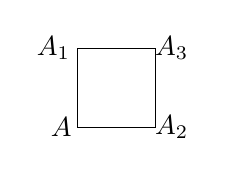
\begin{tikzpicture}
		\draw (0,0) grid (1,1);
		\node (a) at (-0.2, 0) {$A$}; 
		\node (a1) at (-0.3, 1) {$A_1$};
		\node (a2) at (1.2, 0) {$A_2$};
		\node (a3) at (1.2, 1) {$A_3$};
	\end{tikzpicture}
\end{center}
We clearly see that to get from $A \rightarrow A_1$, there is only one way (up), and from $A \rightarrow A_2$, there is only one way (right). So we mark ``1'' onto those vertices, indicating that ``there is 1 way to move from $A$ to those vertices''.
\begin{center}
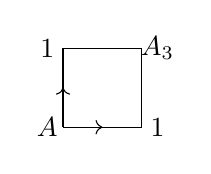
\begin{tikzpicture}
		\draw (0,0) grid (1,1);
		\draw[->] (0,0) -- (0, 0.5);
		\draw[->] (0,0) -- (0.5, 0);
		\node (a) at (-0.2, 0) {$A$}; 
		\node (a1) at (-0.2, 1) {$1$};
		\node (a2) at (1.2, 0) {$1$};
		\node (a3) at (1.2, 1) {$A_3$};
	\end{tikzpicture}
\end{center}
We now focus on the point $A_3$. I know in this example it's obvious that there are two ways to get from $A$ to $A_3$, but here we are going to view it in another way. Since there was one way to get to $A_1$ and one way to get to $A_2$, there must be $A_1+A_2$ ways to get to $A_3$, because those two vertices are the only two points where a person can pass through to get to $A_3$.
\begin{center}
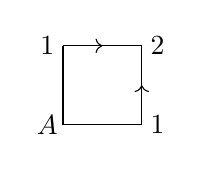
\begin{tikzpicture}
		\draw (0,0) grid (1,1);
		\draw[->] (0,1) -- (0.5, 1);
		\draw[->] (1,0) -- (1, 0.5);
		\node (a) at (-0.2, 0) {$A$}; 
		\node (a1) at (-0.2, 1) {$1$};
		\node (a2) at (1.2, 0) {$1$};
		\node (a3) at (1.2, 1) {$2$};
	\end{tikzpicture}
\end{center}

And here is the generalization, given any grid of $1\times 1$ where the only legal moves are up and right (these rules can be generalized too), the total number of paths into the upper right hand corner vertex is the sum of the number of ways to reach the two vertices that precede it. The figure that illustrates this fact is shown below.
\begin{center}
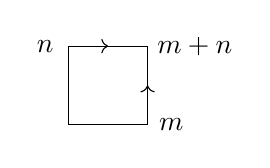
\begin{tikzpicture}
		\draw (0,0) grid (1,1);
		\draw[->] (0,1) -- (0.5, 1);
		\draw[->] (1,0) -- (1, 0.5);
		\node (a1) at (-0.3, 1) {$n$};
		\node (a2) at (1.3, 0) {$m$};
		\node (a3) at (1.6, 1) {$m+n$};
	\end{tikzpicture}
\end{center}
Using this fact, we can fill in our grid from the original problem.
\begin{center}
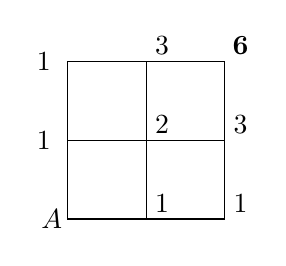
\begin{tikzpicture}
		\draw (0,0) grid (2,2);
		\node (a) at (-0.2, 0) {$A$}; 
		\node (a1) at (-0.3, 1) {$1$};
		\node (a1) at (-0.3, 2) {$1$};
		\node (a2) at (1.2, 0.2) {$1$};
		\node (a3) at (1.2, 1.2) {$2$};
		\node (a3) at (1.2, 2.2) {$3$};
		\node (a2) at (2.2, 0.2) {$1$};
		\node (a3) at (2.2, 1.2) {$3$};
		\node (a3) at (2.2, 2.2) {\textbf{6}};
	\end{tikzpicture}
\end{center}

And we see our answer is 6 total paths. Make sure you understand how to do these grids using this method because this works for \textit{any} path. The more efficient counting method with arranging moves only works for certain grids and will be covered next class.

\subsection{Problems}

\begin{problem}
How many ways are there to walk from $A$ to $B$ if I can only move up or right?
\begin{center}
\begin{tikzpicture}
		\draw (0,0) grid (4,3);
		\node (a) at (-0.3, 0) {$A$}; 
		\node (b) at (4.2, 3) {$B$}; 
\end{tikzpicture}
\end{center}
\end{problem}

\begin{problem}
If a ladybug walks on the segments of the diagram from point A to point B moving only to the right or downward, how many distinct paths are possible?  (\textit{MATHCOUNTS})
\begin{center}
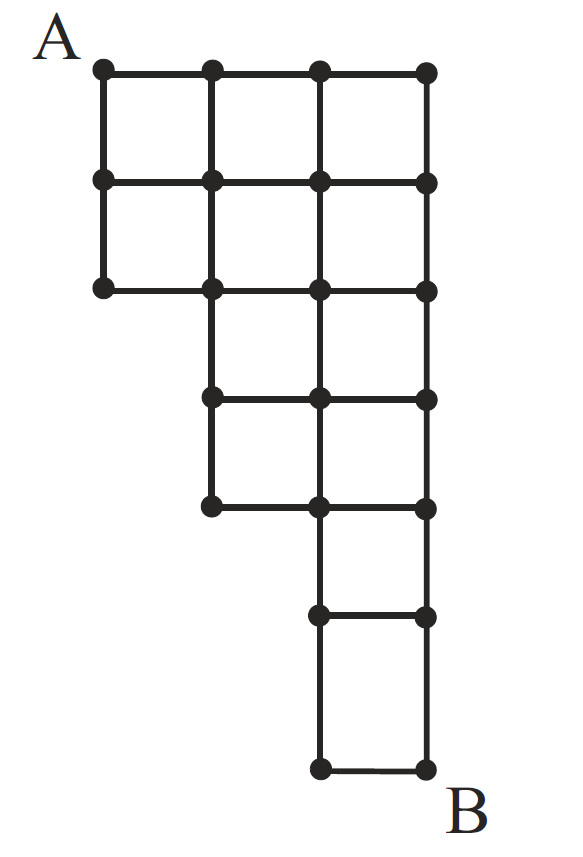
\includegraphics[width=2in]{path}
\end{center}
\end{problem}

\begin{problem}
In the figure below, how many ways are there to select 5 bricks, one in each row, such that any two bricks in adjacent rows are adjacent? (\textit{HMMT})
\begin{center}
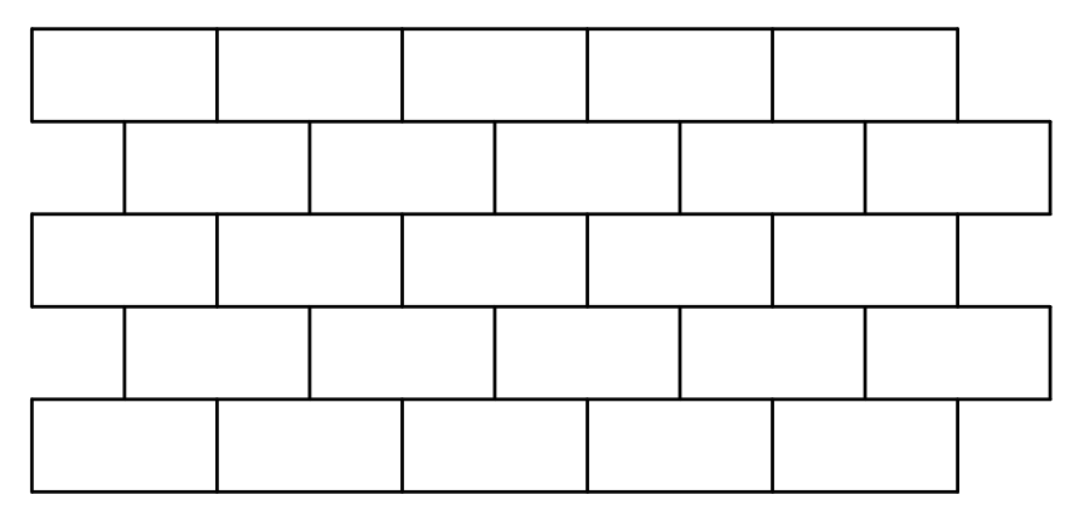
\includegraphics[width=3in]{grid}
\end{center}
\end{problem}

\begin{problem}
How many ways are there to walk from $A$ to $C$ if I must go through point $B$? (hint...you can try labeling the vertices like normal or split the problem into two parts)
\begin{center}
\begin{tikzpicture}
		\draw (0,0) grid (5,3);
		\node (a) at (-0.3, 0) {$A$}; 
		\node (b) at (3.2, 2.2) {$B$};
		\node (b) at (5.2, 3.0) {$C$};
\end{tikzpicture}
\end{center}
\end{problem}

\subsection{A Teaser}
I will leave you guys with an opportunity to see how we can find an easier way to count the number of paths on a grid. Consider any grid of $m\times n$. Then in order to make it from one corner to the other, we must move right exactly $m$ times and up exactly $n$ times. If you want to see this in action, try drawing paths in the diagram below and writing out the letters to the paths you make. For example, in the diagram below, 

\begin{center}
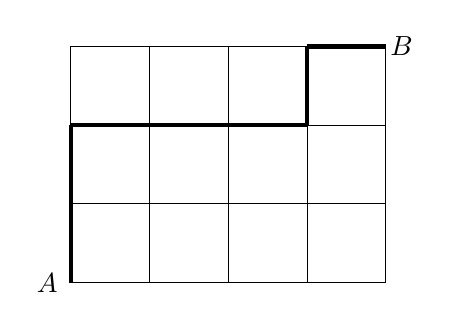
\begin{tikzpicture}
		\draw (0,0) grid (4,3);
		\node (a) at (-0.3, 0) {$A$}; 
		\node (b) at (4.2, 3) {$B$}; 
		\draw[ultra thick] (0,0) -- (0,2);
		\draw[ultra thick] (0,2) -- (3,2);
		\draw[ultra thick] (3,2) -- (3,3);
		\draw[ultra thick] (3,3) -- (4,3);
\end{tikzpicture}
\end{center}

the path can be denoted by the sequence ``UURRRUR''. Using this information, see if you can derive the formula for the number of paths from corner to corner in a $m\times n$ grid.
\newpage

\section{Counting Paths Extended}
\begin{problem}
How many ways can 7 people stand in a line?
\end{problem}

\begin{problem}
I want to order a cake. There are three layers I can put on the cake, and I can choose from 5 different colors. If I cannot repeat any colors, what is the total number of cakes I can make?
\end{problem}

\begin{problem}
A regular icosahedron is a $20$-faced solid where each face is an equilateral triangle and five triangles meet at every vertex. The regular icosahedron shown below has one vertex at the top, one vertex at the bottom, an upper pentagon of five vertices all adjacent to the top vertex and all in the same horizontal plane, and a lower pentagon of five vertices all adjacent to the bottom vertex and all in another horizontal plane. Find the number of paths from the top vertex to the bottom vertex such that each part of a path goes downward or horizontally along an edge of the icosahedron, and no vertex is repeated. (\textit{Source: AIME I \#3 2016})
 \begin{center}
 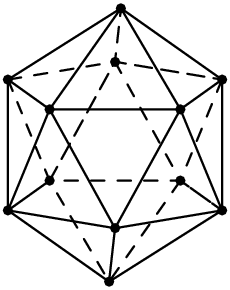
\includegraphics[width=2in]{iso}
 \end{center}
\end{problem}

\begin{problem}
Of the 15 players on a soccer team, 13 are starters. How many different teams of 13 starters are possible?
\end{problem}

\begin{problem}
How many ways can I arrange the word ``MATHCOUNTS''?
\end{problem}

\begin{problem}
How many ways can I arrange the word ``MISSISSIPPI''?
\end{problem}

\begin{problem}
How many ways can I arrange the word ``VIRGINIA'' if the V always has to be next to the A? (e.g. ``VAIRGINI'' or ``GINAVIRI'' both work)
\end{problem}

\begin{problem}
If I want to put 7 balls in a row, 2 that are red, 3 that are blue, and 2 that are green (same colors are indistinguishable), how many ways can I do so?
\end{problem}

\begin{problem}
 How many ways are there to get from the lower left hand corner to the upper right hand corner of the grid below by only using moves that are right or up?
 \begin{center}
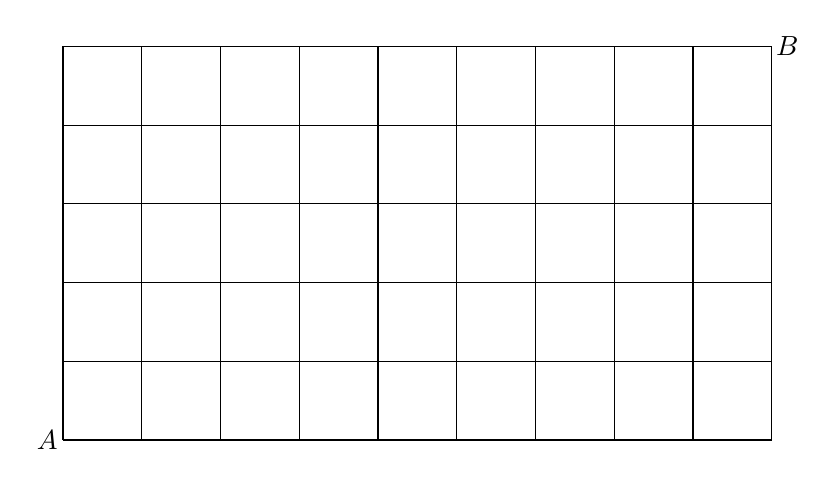
\begin{tikzpicture}
		\draw (0,0) grid (9,5);
		\node (a) at (-0.2, 0) {$A$}; 
		\node (b) at (9.2, 5) {$B$}; 
\end{tikzpicture}
\end{center}
\end{problem}

\begin{problem}
 I am currently at home ($A$) and I want to make my way to work at $B$. However, I know there is an accident at point $C$ and $D$ in the city, so I want to avoid routes that pass through those places. Taking this into consideration, how many ways can I drive from $A$ to $B$ if I must not pass through $C$ \textit{or} $D$?
 \begin{center}
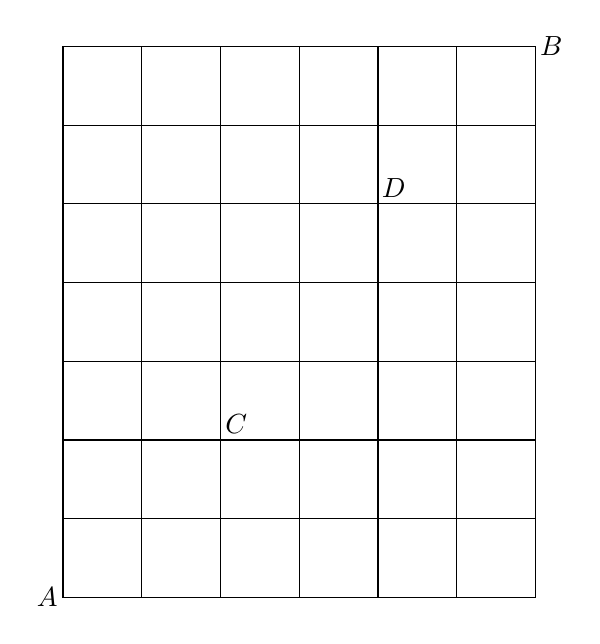
\begin{tikzpicture}
		\draw (0,0) grid (6,7);
		\node (a) at (-0.2, 0) {$A$}; 
		\node (c) at (2.2, 2.2) {$C$};
		\node (d) at (4.2, 5.2) {$D$};
		\node (b) at (6.2, 7) {$B$}; 
\end{tikzpicture}
\end{center}
 \end{problem}

\begin{problem}
I am walking a 3-D grid. If I want to get from (0,0,0) to (2,5,4), how many paths are possible?
\end{problem}

\begin{problem}
$^{\ast \ast \ast}$ Dizzy Daisy is standing on the point (0, 0) on the $xy$-plane and is trying to get to the point (6, 6). She starts facing rightward and takes a step 1 unit forward. On each subsequent second, she either takes a step 1 unit forward or turns 90 degrees counterclockwise then takes a step 1 unit forward. She may never go on a point outside the square defined by $\abs{x} \leq 6, \,\, \abs{y} \leq 6$, nor may she ever go on the same point twice. How many different paths may Daisy take? (\textit{Source: HMMT})
\end{problem}
\newpage

\section{Recursion}
The purpose of this document is to provide practice for doing basic recursion calculations.

\subsection{Introduction}
We are interested in calculating values for a recurrence relation described by:
\begin{equation}
    a_n = c_{n-1}a_{n-1}+c_{n-2}a_{n-2}+\cdots+c_0a_0
\end{equation}
where $a_i$ is a term in the sequence $\{a_i\}_{i=1}^{N}$, and $c_i$ is some function (it's usually a constant for our purposes).

In order to be able to build up our sequence $\{a_i\}_{i=1}^{N}$, all we need to do is have the necessary \textbf{initial conditions}, and then use the \textbf{recurrence relation} to figure out more terms. 

\subsubsection{Initial Conditions}
What I mean by initial condition is the starting values you use for your sequence. If you don't have the necessary information to compute the next term, then how will you be able to find more terms? For example, let's say our recurrence relation was

\begin{equation}
    a_n = 3a_{n-2}+4a_{n-2}, \quad n\geq2, a_0 = 2
\end{equation}

We can try to figure out $a_2$, but what we quickly realize is 

$$a_2 = 3a_1+4a_0 = 3(???)+8$$

...we are stuck and we can't continue. This is what I mean by you need sufficient initial conditions in order to figure out the entire sequence. 

Another example that gives you partial information about the sequence rather than the entire sequence is when there is some sort of parity involved. Consider this example:

\begin{equation}
    a_n = 2a_{n-2}, \quad n\geq 2, a_0=3
\end{equation}
We can easily compute that $a_2=6, a_4=12, a_6=24, ...$, but we don't know anything about the odd terms! Therefore, even though we are able to get an infinite sequence from our initial conditions, it isn't \textit{complete} enough so that we can figure out the entire sequence. These type of sequences appear in many applications, including solving for coefficients in solutions of differential equations.

\clearpage

\subsection{Problems}
Compute the first couple terms of the following recurrence relations (fill out the table)

\begin{problem}
\begin{equation}
    a_n = a_{n-1}+a_{n-2}, \quad n\geq2, a_0=1, a_1=1
\end{equation}
\begin{table}[H]
    \renewcommand{\arraystretch}{1.5}
    \centering
    \begin{tabular}{|c|D{1in}|}
        \hline
        $n$ & $a_n$ \\ \hline
        2 &  \\ \hline
        3 & \\ \hline
        4 & \\ \hline
        5 & \\ \hline
        6 & \\ \hline
        7 & \\ \hline
        8 & \\ \hline
    \end{tabular}
\end{table}

Does this sequence look familiar?
\end{problem}

\begin{problem}
\begin{equation}
    a_n = a_{n-1}+a_{n-2}, \quad n\geq2, a_0=2, a_1=4
\end{equation}
\begin{table}[H]
\renewcommand{\arraystretch}{1.5}
    \centering
    \begin{tabular}{|c|D{1in}|}
        \hline
        $n$ & $a_n$ \\ \hline
        2 &  \\ \hline
        3 & \\ \hline
        4 & \\ \hline
        5 & \\ \hline
        6 & \\ \hline
        7 & \\ \hline
        8 & \\ \hline
    \end{tabular}
\end{table}

Why doesn't this look like Fibonacci even though it's defined the exact same way?
\end{problem}

\clearpage

\begin{problem}
\begin{equation}
    a_n = 2a_{n-1}, \quad n\geq2, a_0=1
\end{equation}
\begin{table}[H]
\renewcommand{\arraystretch}{1.5}
    \centering
    \begin{tabular}{|c|D{1in}|}
        \hline
        $n$ & $a_n$ \\ \hline
        2 &  \\ \hline
        3 & \\ \hline
        4 & \\ \hline
        5 & \\ \hline
        6 & \\ \hline
        7 & \\ \hline
        8 & \\ \hline
    \end{tabular}
\end{table}

Can you guess the explicit formula for $a_n$? (so for example $a_n = 3n$ is explicit and not recursive (not dependent on previous terms))
\end{problem}

\begin{problem}
\begin{equation}
    a_n = 2a_{n-1}-4a_{n-2}+9a_{n-3}, \quad n\geq3, a_0=-1, a_1=2, a_2=-3
\end{equation}
\begin{table}[H]
\renewcommand{\arraystretch}{1.5}
    \centering
    \begin{tabular}{|c|D{1in}|}
        \hline
        $n$ & $a_n$ \\ \hline
        3 & \\ \hline
        4 & \\ \hline
        5 & \\ \hline
        6 & \\ \hline
        7 & \\ \hline
    \end{tabular}
\end{table}
\end{problem}

If you want, you can figure out a \textit{linear recurrence} for most of these problems. The process for figuring that out is explained in the recursion lecture.
\newpage

\section{Introduction to Geometry}
\subsection{Drawing}
Try to draw the following:

\begin{enumerate}
    \item Given a point $P$, draw all points that are exactly 2 inches away from $P$. What shape is this? (Note: the \textbf{locus} of points is a set of points that satisfies a particular condition. E.g. for this problem, we are finding the locus of points that have distance 2 in from $P$)
    \item Draw three points and make them
        \begin{enumerate}
            \item All \textit{collinear} (lie on a single line)
            \item Not all \textit{collinear}. If you connect all of these points to each other, how many lines do you get? (is it in the form of $\binom{n}{2}$?) Do you create an enclosed region? What is this shape called?
            \item In general, if you have $n$ non-collinear points, how many distinct line segments can you draw?
            \item $^{\ast \ast \ast}$ A \textit{diagonal} of a polygon is defined to be a line from a vertex to another distinct vertex that is not adjacent to it (or else it'd just be the side). Given what we just did in the part before, derive the formula for the number of diagonals in a $n$-sided convex polygon.
        \end{enumerate}
    \item Draw a \textit{convex} quadrilateral---a four-sided shape with all interior angles $<180^{\circ}$
    \item Draw a \textit{concave} quadrilateral---a four-sided shape with one interior angle $>180^{\circ}$
    \item Is it possible to draw a concave triangle? (\textit{Hint: Look at proof \#1 and think about the definition of a concave polygon})
\end{enumerate}

\subsection{Proofs}
Let's try proving some basic facts. For these proofs, you will need to know the basic angle theorems (opposite side angles are equal, parallel line transversals) and the triangle congruence theorems (SSS, SAS, AAS).
\begin{enumerate}
    \item Prove that the interior angles of a triangle sum to $180^{\circ}$ \textit{(Hint: draw line $\overline{AB}$, and draw a line parallel to $\overline{AB}$ that goes through $C$)}
    \item Prove that the sum of the interior angles of \textit{any} $n$-sided polygon (convex or concave) sum to $(n-2)180^{\circ}$. (\textit{Hint: What shape do we know the sum of the angles of?})
    \item Prove that if a triangle has 2 equal sides, it must also have two equal angles. This triangle is called isosceles because it has two equal sides. (\textit{Hint: bisect the angle that is not equal to the other two. You should get two congruent triangles.}) Once you prove this, you should be able to prove the converse (if two angles are equal in a triangle, then two sides must also be equal) very easily.
    \item Given that the area of a triangle is $\frac{1}{2} b h$, where $b$ is the base and $h$ is the height, derive the formula for a trapezoid, which is $\frac{b_1+b_2}{2}h$, where $b_1, b_2$ are the two bases, and $h$ is the height. (\textit{Hint: Split the trapezoid into two triangles})
\end{enumerate}
\newpage
\section{Game Theory in Action}
We will be playing some games introduced last lesson to get a better feel for what game theory is about. We will learn about strategies and see how some of the results we derived last class happen because of strategy optimization.

\subsection{The Games}
We will explore the following games today:
\begin{itemize}
    \item Traditional Dice Games
    \item Monty Hall
    \item Prisoner's Dilemma
    \item Oligopoly Simulation
\end{itemize}

\subsection{Dice}
This is one of the most popular one-player games out there. Remember, for these type of games, the main question is always ``what is my expected earnings?'' This will let you determine how much you should pay to play the game to you don't get ripped off.

\begin{gm}
Suppose we play a game so that each time you roll a standard dice, you win the amount of dollars that you roll. What is the expected amount of dollars you win every roll?
\end{gm}

\begin{gm}
In the game of $\text{Dice}^2$, you can win money by rolling dice! Your winnings are determined by the product of the two numbers that appear on the pair of dice you roll. \textit{Extension: Can you figure out the expected winnings of a general $Dice^n$ game?}
\end{gm}

\subsection{Monty Hall}
Of course, we'll play the classic Monty Hall first to see what the craze is all about.

\begin{gm}
Suppose we have 3 curtains, 2 with goats and 1 with a car behind it. You are given the option to choose any curtain at the beginning. Then, the host removes one of the remaining two curtains that has the goat behind it so that you are left with two curtains, one with the car and one the goat. You are given the option to switch at the end.
\end{gm}

\begin{gm}
Suppose we play Monty Hall with 4 goats and 1 car. Find the probability you win if you switch.
\end{gm}

\begin{gm}
Suppose we play Monty Hall with 4 goats and 2 cars. After you choose a curtain, the host removes all but your curtain and another curtain so that only one goat and one car is left. Find the optimal strategy and your probability of winning with this strategy.
\end{gm}

\begin{gm}
Suppose we play Monty Hall with 2 goats and 2 cars. After you choose a curtain, the host removes all but your curtain and another curtain so that only one goat and one car is left. Find the optimal strategy and your probability of winning with this strategy.
\end{gm}

\subsection{Prisoner's Dilemma}
Ah...the most nerve-racking and evil game of all. You'll be pitted against your own morals when you try these out...

\begin{gm}
We will begin with the classic Prisoner's Dilemma. Person A and Person B are in trouble at school, but the principal is not sure what happened. The following are the options for Person A and Person B and their payoffs.
\begin{center}
\renewcommand{\arraystretch}{1.5} % Default value: 1
\begin{tabular}{cc|c|c}
     &\multicolumn{3}{c}{Person A} \\
     && Tattle & Keep Quiet \\
     \cline{2-4}
     \multirow{2}{*}{Person B}&Tattle & 5 days, 5 days & Blame Cleared, Expelled \\
     &Keep Quiet & Expelled, Blame Cleared & 1 day, 1 day
\end{tabular}
\end{center}
\end{gm}


\begin{gm}
The following is the payoff matrix for two companies who are deciding whether or not to advertise for the upcoming year.
\begin{center}
\renewcommand{\arraystretch}{1.5} % Default value: 1
\begin{tabular}{cc|c|c}
     &\multicolumn{3}{c}{Company A} \\
     && Advertise & Don't Advertise \\
     \cline{2-4}
     \multirow{2}{*}{Company B}& Advertise & (\$10, \$10) & (\$19, \$6) \\
     &Don't Advertise&(\$10, \$7) & (\$15, \$17) 
\end{tabular}
\end{center}
\end{gm}

\begin{gm}
The following is the payoff matrix for two companies who are deciding whether or not to advertise for the upcoming year.
\begin{center}
\renewcommand{\arraystretch}{1.5} % Default value: 1
\begin{tabular}{cc|c|c}
     &\multicolumn{3}{c}{Company A} \\
     && Advertise & Don't Advertise \\
     \cline{2-4}
     \multirow{2}{*}{Company B}& Advertise & (\$10, \$10) & (\$19, \$6) \\
     &Don't Advertise&(\$10, \$7) & (\$15, \$17) 
\end{tabular}
\end{center}
\end{gm}

\begin{gm}
You and your friend are going trick-or-treating. You guys are trying to figure out what paths to take. If you guys take the same path, then you will both receive less candy than if you guy choose different paths.
\begin{center}
\renewcommand{\arraystretch}{1.5} % Default value: 1
\begin{tabular}{cc|c|c}
     &\multicolumn{3}{c}{Person 1} \\
     && Route A & Route B \\
     \cline{2-4}
     \multirow{2}{*}{Person 2}& Route A & (30, 40) & (70, 100) \\
     &Route B&(90, 70) & (40, 30) 
\end{tabular}
\end{center}
\end{gm}

\subsubsection{Golden Balls}
\begin{gm}
I bring to you the British game show---Golden Balls! This show used to air on TV from 2007-2009, and was one nervous game for contestants and spectators alike. In the final round, we reach the infamous ``Split or Steal'' situation, which is described by the following matrix:
\begin{center}
\renewcommand{\arraystretch}{1.5} % Default value: 1
\begin{tabular}{cc|c|c}
     &\multicolumn{3}{c}{Person 1} \\
     && Split & Steal \\
     \cline{2-4}
     \multirow{2}{*}{Person 2}& Split & (Half, Half) & (Nothing, Everything) \\
     &Steal &(Everything, Nothing) & (Nothing, Nothing) 
\end{tabular}
\end{center}
\end{gm}

\subsection{Oligopoly Simulations}
In this section we'll see the two-player game extended in general to larger scales.

\subsubsection{Extra Credit}
\begin{gm}
Suppose I am offering you extra credit. I am giving you 10 points...but what you can do is keep the points, which are added directly to your grade, or donate them to charity, which doubles the points and is then distributed among everybody else. For example, I could keep 5 points and donate 5 points to charity, which would put $5\times2 = 10$ points into the pot to be distributed to everyone.
\end{gm}

\subsubsection{Product Market}
\begin{gm}
You guys are all CEOs of major companies that are competing in one market. Each round, you will be shown a supply and demand graph, telling you how much you will sell your product for given a certain quantity supplied of the product. What you have to decide is how much of the product to produce? You each are given a card that tells you your cost of production of one product. The quantity supplied in the market is the sum of the productions of all the companies combined.

Use the following table to keep track of your production, costs, and profits in each round.

\begin{center}
\renewcommand{\arraystretch}{2.5} % Default value: 1
\begin{tabularx}{.9\textwidth}{|c|c|c|c|X|}
    \hline
    Round & Production Cost & \# Produced & Market Price & Profit \\
    \hline
    1&&&& \\
    \hline
    2&&&& \\
    \hline
    3&&&& \\
    \hline
    4&&&& \\
    \hline
    5&&&& \\
    \hline
\end{tabularx}
\end{center}

\vspace{0.2in}

\hspace{2.74in} \textbf{Total Profit: } \underline{\hspace{5.5cm}}

\end{gm}
\newpage
\chapter{A Potpourri of Problems}
\section{Mega Review for 2014-15}
To conclude the first semester of our class with a bang, we will review all of the major categories we covered so far. Since there is not much space on this document, I recommend doing all work on a separate sheet of paper (and you can put your answers there too).
	\subsection{Counting}
		We did most of our counting through the AoPS videos. These videos are very helpful (and entertaining!) so they should have taught you some good counting skills. Let's take a look at a few of them:
		\begin{enumerate}
			\item How many numbers are in the set $\{-9, -7, \cdots, 199\}$
			\item How many multiples of 7 are there between 183 and 937?
			\item If I have 4 salads and 3 meats, how many meals can I make of 2 salads and 2 meats if order does not matter?
			\item If there are 8 horses in a race, how many ways are there for them to finish $\nth{1}$, $\nth{2}$ and $\nth{3}$? 
			\item How many ways are there to arrange the letters of ``DISNEY''?
			\item 5!
			\item 6!
			\item 7!
			\item 8!
			\item 9!
			\item 10!
			\item ${874 \choose 0}$ 
			\item ${959 \choose 1}$ 
			\item ${9 \choose 7}$ 
			\item ${19 \choose 3}$ 
			\item ${9999 \choose 9998}$ 
			\item How many ways can I walk from (0, 0) to (6, 7) on a grid?
			\item With the same $6 \times 7$ grid, how many of these paths go through (3, 4)?
			\item With the same $6 \times 7$ grid, how many of these paths go through (3, 4) and (6, 5)?
			\item How many ways can I walk along the edges of a 3x3x3 cube? (I can go through the center)
			\item How many ways can I walk along the surface of a 2x2x2 grid (I \textbf{cannot} go into the center)?
		\end{enumerate}
	\subsection{Number Theory}
		 The bulk of what we covered this year was in Number Theory---these techniques help you understand numbers better so you can work with math more proficiently.
		\subsubsection{Factors}
			\begin{enumerate}
				\item What number do I have to put in 482\_8 to make it divisible by 3 and 4?
				\item Given 180:
				\begin{enumerate}
					\item How many positive factors does it have?
					\item How many even factors does it have?
					\item How many odd factors does it have?
					\item How many perfect square factors does it have?
					\item What are the sum of the factors of it?
					\item Do (a)-(e) for 108, 576, 1296
				\end{enumerate}
				\item What is the largest power of 2 that divides 45!?
				\item What is the largest power of 4 that divides 45!?
				\item What is the largest power of 5 that divides 45!?
				\item Completely prime factorize 20!
				\item Why do perfect squares always have an odd number of factors?
				\item Is 0 divisible by anything? Everything?
			\end{enumerate}
		\subsubsection{Modular Arithmetic}
			\begin{enumerate}
				\item What is the last digit of $2^{2842}$?
				\item What is the last digit of $3^{1958^{1842}}$
				\item What is the last digit of $1382^{2842}$
				\item What is the last digit of $\sum_{i=1}^\infty i! = 1!+ 2!+3!+4!+5!+\cdots$
				\item What is the last digit of $1928999936!$ ?
				\item What is the remainder when $23+49+82-71$ is divided by 8?
				\item What is the remainder when $2938493 + 17329 + 4889382$ is divided by 4?
				\item What is the remainder when $3\times 8 \times 11$ is divided by 5?
				\item What is the remainder when $1248963 \times 242448481 \times 964836123 \times 24363636967$ is divided by 12?
				\item What is the smallest positive integer that has a remainder of 3 when divided by 5 and a remainder of 2 when divided by 17?
				\item What is the smallest positive integer that has a remainder of 2 when divided by 4, 5, 6, 7, and 8?
				\item What is the smallest positive integer that has a remainder of 4 when divided by 5, 7 when divided by 8, 12 when divided by 13 and 18 when divided by 19?
			\end{enumerate}
		\subsubsection{Sense}
			You've already seen very extreme cases that number sense can deal with. This section has problems that you will \textbf{definitely} see more often than something like $25 \times 18378275208$ but also has the extreme cases anyway for review.
			\begin{enumerate}
				\item $5 \times 135678992$
				\item $5 \times 48527888$
				\item $25 \times 96385264$
				\item $25 \times 123456789$
				\item $15 \times 32$
				\item $25 \times 45$
				\item $11 \times 19$
				\item $34 \times 36$
				\item $22 \times 41$
				\item $17 \times 71$
				\item $13 \times 34$
				\item List all all the squares from $1$ to $40$
				\item $85^2$
				\item $285^2$
				\item $65^4$
				\item $3 \times 142857$
				\item $\frac{184}{7}$ in decimal form
				\item $13 \times 17$
				\item $22 \times 34$
				\item $92 \times 98 \times 3$
				\item $37 \times 43$
				\item $98 \times 107$
			\end{enumerate}
	\subsection{Algebra}
		\begin{enumerate}
			\item If kid tickets cost \$2 and adult tickets cost \$3, how many kids and adults are there in a group of 86 people that spends \$244 total?
			\item $(a+b)^2 = $
			\item $(a-b)^2 = $
			\item $(a+b)^3 = $
			\item $(a+b)^3 = $
			\item $(a+b)^4 = $
			\item $(a+b)^4 = $
			\item Do you think the coefficients of the expansions above look like Pascal's triangle? If so, try to figure out what $(a+b)^5$ looks like and figure out in general what $(a+b)^n$ will look like
			\item $a^2-b^2 = $
			\item $a^3+b^3 = $
			\item $a^3-b^3 = $
			\item What is the largest prime factor of $82^{2}-62^{2}$?
			\item $\frac{8x}{7} + 8 = -19$
			\item $5x^{2} = 80$
			\item $\sqrt{9620}$
			\item $(\sqrt{8})^{\frac{25}{6}}$
			\item $\frac{1-\sqrt{15}}{\sqrt{5}-2}$ 
			\item $\frac{\sqrt{7}+\sqrt{3}}{\sqrt{18}-\sqrt{14}}$
			\item Estimate the value of $x$, if $\frac{1}{x} +1 = \sqrt[3]{3}$
			\item Compute $\sum\limits_{i=1}^{15} i$ \par
			\item Compute $\sum\limits_{i=8}^{28} 5$ \par
			\item Compute $\sum\limits_{i=1}^{\infty} \frac{1+3^{k}}{4^{k}}$ \par
			\item Compute $\prod\limits_{i=1}^{10} \frac{i}{i+2}$
			\item Estimate $0.99^{1839}$
			\item Estimate $1.002^{2752}$

		\end{enumerate}
			\subsection{Geometry}
		Mostly areas you should know for geometry---and of course the Pythagorean theorem. Since we did not get through much, I will not include many problems here.
		\begin{enumerate}
			\item What is the area of a square with side length $8\sqrt{2}$?
			\item What is the area of an equilateral triangle with side length $2-\sqrt{3}$
			\item A right triangle with hypotenuse 13 and one of its legs 5
			\item Area of a circle with diameter 5
			\item Area of a trapezoid with bases 3 and 4, and height 8
			\item Area of a rectangle with side lengths 14 and 3
			\item What is the hypotenuse of a triangle with legs 18 and 34?
			\item What is the area of an equilateral triangle inscribed inside a circle of radius 4?
			\item Find the distance from (-1, 8) to (9, 4)
			\item The measure of an interior angle of a regular 18-gon
			\item A cylindrical tank with height 17 m and radius 8 m is filled at the rate of 37 L/hour. The tank is being drained at 22 L/min. How long will it take to fill the tank? Note: there are 1000 liters per cubic meter
			\item A toy house consists of a 4 in cube with a square pyramid of height 2 in on top. What is the total volume of this house?
		\end{enumerate}
\newpage
\section{Pi Day 3/14/16}
\begin{enumerate}
    \item Seven Kevins are trying to figure out how to place seven pies on a table, which has a $9\times 9$ grid marking as shown below:
    \begin{center}
    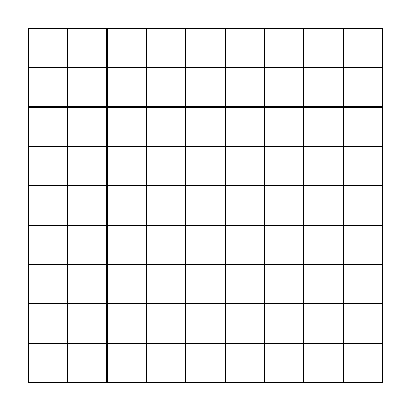
\begin{tikzpicture}[scale=0.50]
    		\draw (0,0) grid (9,9);
    \end{tikzpicture}
    \end{center}
    The Kevins will put the each of the seven pies into a square, but since they are picky, they will only be satisfied with the pie arrangement if no two pies share a row or column. How many arrangements satisfies this condition? (assume pies are indistinct)
    \item Today, Samuel the Lamuel is feeling particularly charitable, and wants to cut his pie into some some pieces so he can share with his good folks. Given that a a pie is a 3-D object, and cuts are assumed to be straight (like a plane), what is the minimum number of cuts he needs to make in order to serve a crowd of 100 people?
\end{enumerate}
\end{document}
